\documentclass[twoside,11pt]{article}

\usepackage[implicit=false]{hyperref}

\usepackage{jair, theapa, rawfonts}

\usepackage[pdftex]{graphicx}
\DeclareGraphicsExtensions{.pdf,.jpeg,.png}

\usepackage{amsmath,amsfonts,amssymb,amscd,amsthm,xspace}
\usepackage{array}

\usepackage{multirow}
\usepackage{times}
\usepackage{breqn}
\usepackage{hyperref}

\hyphenation{spe-ci-fi-cal-ly re-gu-la-ted ge-ne-ra-li-sa-ti-on fun-ding dif-fe-rent pa-ra-me-ter a-ve-ra-ging ha-ving bia-ses va-lu-es in-fe-ren-ce theo-rem pro-ba-bi-li-ty ap-pro-xi-ma-ti-on ma-xi-mi-sing u-sing e-le-ments de-fi-ni-ti-on}

\DeclareMathOperator*{\argmax}{arg\,max}


\jairheading{1}{2022}{1-29}{11/21}{--/--}
\ShortHeadings{Counting Reliably with Unreliable Sensors: POPP for Robot Exploration}{}
% {Jovan, Mariya, Hawes \& Wyatt}
\firstpageno{1}

\begin{document}
	
\newcommand{\tp}{\textrm{\textit{tp}}}
\newcommand{\fp}{\textrm{\textit{fp}}}
\newcommand{\tpr}{\textrm{\textit{tpr}}}
\newcommand{\fnr}{\textrm{\textit{fnr}}}
\newcommand{\fpr}{\textrm{\textit{fpr}}}
\newcommand{\tnr}{\textrm{\textit{tnr}}}
\newtheorem{definition2}[subsection]{Definition}	

\title{Counting Reliably with Unreliable Sensors: Partially Observable Poisson Processes for Robot Exploration}

\author{%\name Steven Minton \email minton@ptolemy.arc.nasa.gov \\
       %\name Andy Philips \email philips@ptolemy.arc.nasa.gov \\
       %\addr NASA Ames Research Center, Mail Stop: 244-7,\\
       %Moffett Field, CA  94035 USA
       %\AND
       %\name Mark D. Johnston \email johnston@stsci.edu \\
       %\addr Space Telescope Science Institute,
       %3700 San Martin Drive,\\
       %Baltimore, MD 21218 USA
       %\AND
       %\name Philip Laird \email laird@ptolemy.arc.nasa.gov \\
       %\addr NASA Ames Research Center,
       %AI Research Branch, Mail Stop: 269-2,\\
       %Moffett Field, CA  94035 USA
   }

% For research notes, remove the comment character in the line below.
% \researchnote

\maketitle


%!TEX root = ../bare_jrnl.tex

\begin{abstract}
	
	

    % We present practical Bayesian inferences and exploration methods for count data collected by autonomous robots with unreliable sensors in human-populated environments. It addresses the problem of drawing incorrect inferences from unreliable count data which affects the effectiveness of robot exploration in maximizing its interaction with humans. Two contributions are presented in this paper: (1) A set of inference methods for a Poisson process which takes into account the unreliability of the robotic sensory systems used to count events is proposed, investigated, and empirically tested. The actual posterior distribution of such Poisson processes is estimated via two tractable approximations. Variations of these processes are presented, in which (i) sensors are uncorrelated, (ii) sensors are correlated, (iii) the unreliability of the observation model, when built from data, is accounted for. (2) Several exploration methods based on optimistic predictions from the resulting posteriors of contribution (1) are proposed, and empirically evaluated. They are assessed by the way they improve the number of human encounters the robot experiences. The results indicate that addressing the unreliable sensors improve human encounters by at least a factor of 2.   

Consider a mobile robot exploring an office building with the aim of observing as much human activity as possible over several days. It must learn where and when people are to be found, count the observed activities, and revisit popular places at the right time. In this paper we present a series of Bayesian estimators for the levels of human activity that improve on simple counting. We then show how these estimators can be used to drive efficient exploration for human activities. The estimators arise from modelling the human activity counts as a partially observable Poisson process (POPP). This paper presents novel extensions to POPP for the following cases: (i) the robot's sensors are correlated, (ii) the robot's sensor model, itself built from data, is also unreliable, (iii) both are combined. It also combines the resulting Bayesian estimators with a simple, but effective solution to the exploration-exploitation trade-off faced by the robot in a real deployment. A series of 15 day robot deployments show how our approach boosts the number of human activities observed by 70\% relative to a baseline and produces more accurate estimates of the level of human activity in each place and time.

    % The Poisson assumption is a popular choice when data arises in the form of counts. In many applications, such as in mobile robotics, such counts are prone to systematic error due to noisy sensors and perception algorithms. In this paper we present a collection of Bayesian estimators for the \emph{partially observable} variant of the Poisson process (POPP) which address this problem. The presented estimators deal with cases in which (i) the sensors are uncorrelated, (ii) the sensors are correlated, and (iii) the unreliability of the observation model, when built from data, is accounted for. The resulting posterior is used to drive exploration of a mobile robot with unreliable sensors. We also present an empirical analysis showing the benefit of correcting miscounts in both real and synthetic data, and robot exploration.  
\end{abstract}

%\begin{IEEEkeywords}
%Poisson processes, partial observability, misclassified counts, robot exploration.
%\end{IEEEkeywords}

%Automated control of a stochastic process requires estimates of both aleatoric and epistemic uncertainty. These allow rational choice between exploration to reduce epistemic uncertainty and optimisation of performance in the face of aleatoric uncertainty. This is true for domains as diverse as optimal drug trial design, efficient routing while learning a map, or maximing performance while learning to play a game.

%!TEX root = ../bare_jrnl.tex


\section{Introduction}
\label{sec:introduction}

Autonomous mobile robots are being developed to operate in human populated spaces, such as homes and offices~\cite{hawes2016strands}. It is useful for these robots to predict patterns of human activity, so as to learn about those activities~\cite{coppola2016learning,duckworth2016a} or to plan interactions with humans~\cite{2020AAMAS_street}. This paper is concerned with how a robot can correctly estimate how many human activities it has encountered, predict how many will occur in a particular location at a particular time, and then use these to optimize the exploration-exploitation trade-off that occurs during active learning, so as to observe as many human activities as possible during a deployment.

Consider a mobile service robot that works in a large office building. Let us suppose that one of the system designers' aims is for the robot to observe and thereby learn about the various activities performed by humans, and for this learning to have to occur over several days or weeks. To achieve this goal, the robot must learn where and when people are to be found, count the observed activities (perhaps grouped by their categories), and revisit places at times when those activities can be observed in sufficient number. For example, to learn about eating activities the robot would benefit from visiting the canteen at lunchtime, rather than at the start of the day. If such a robot is to be deployed to a variety of buildings, without re-programming of rules by hand, it should autonomously learn the spatio-temporal distribution of these activities and exploit that learning to observe a useful variety and number of activities.

This involves solving two problems. First, the robot must estimate where it can observe the greatest number of human activities at each time of the day. Second, as the robot is learning it should trade-off exploring for new time-place combinations where it might discover a high-level of human activity and re-visiting those time place combinations where it already knows that a wealth of human activity is to be found. This second problem involves solving an exploration-exploitation trade-off. 

\begin{figure}[t!]
	\centering

	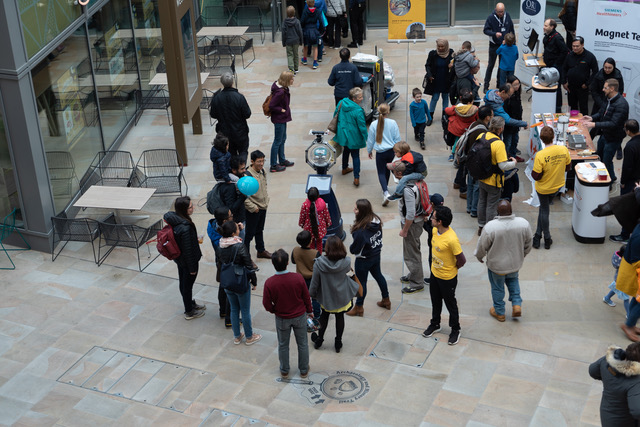
\includegraphics[width=0.79\textwidth]{./figures/robot_in_human_environment.jpeg}
	\caption{Our mobile robot observes people at an event.} 
	\label{fig:robot_in_human_environment}
\end{figure}
This paper presents a Bayesian method to solve both these problems in the case where we treat human activities as count data. %In this approach, there are two sources of uncertainty regarding the number of activities found: human behaviour which has some inherent uncertainty (aleatoric uncertainty) and the robot's uncertainty about what it observed due to it's unreliable sensing (epistemic uncertainty). By representing both types of uncertainty, 
The Bayesian framework models not only the frequency of human activities and the variation in this, but also the robot's uncertainty about the mean rate at which activities occur. Thus, the Bayesian estimator captures both inherent process uncertainty (aleatoric uncertainty) and the robot's additional uncertainty in what it knows about the process (epistemic uncertainty). It can also correct for inherent biases (a tendency to false positives or false negatives in the sensory system). Because of this it has two advantages over a baseline frequentist estimator. First, it will produce more accurate estimates and predictions of human activity levels than a method that does not model classification errors. Second, because it captures epistemic uncertainty it can be used to perform active learning. This active learning problem is fundamentally an exploration-exploitation trade-off. Should the robot visit a place at a time such that it can exploit what it already knows about the likely activity level, or should it explore a place-time combination about which it knows less, but about which it might learn and so lead to a higher rate of activity observation in the long run? This active learning problem is intractable in the strict formulation, since it involves reasoning over a tree of possible knowledge states. Despite this, there are effective, heuristic active-learning rules that are quick to evaluate. %Our main experimental contribution is an active learning scenario in which the robot must learn to efficiently explore a public space so as to learn about human activities quickly.

%The Bayesian framework enables the robot to draw better inferences about the typical level of activity in a particular place time. The Bayesian estimator lends itself to a simple yet effective solution to the exploration-exploitation problem. 
We develop a series of Bayesian estimators. Then we present a method to use these to drive exploration. This uses both a Fourier transform to capture the periodicity of human activities and the epistemic uncertainty in the activity rate as captured by the posterior. Using this estimation, prediction and exploration technique, we then present the results of several long-run deployments of a real robot in a public building. These long-run deployments (15 days per treatment) are used to test whether the different Bayesian estimators, together with the solution to the exploration-exploitation trade-off, result in the robot observing greater numbers of human activities than a baseline frequentist method.

%Our mobile robot has multiple sensors and perception algorithms used to detect humans performing activities. These are inevitably somewhat unreliable. Thus, the raw counts arising from the detectors will be wrong. But, by learning statistical models of the sensor unreliability, the robot can partially correct for these miscounts. In other words, we can teach the robot to count humans more reliably than the raw counts from its detectors. 
This paper builds on our earlier work, which showed how to count reliably from a single unreliable detector or from multiple, unreliable, uncorrelated detectors~\cite{jovan18a}. That work formulated the problem as Bayesian inference for a \textit{partially observable Poisson process} (POPP) and showed an improvement on a baseline model assuming sensor reliability, termed the fully observable Poisson process (FOPP).

This paper makes the following technical contributions. First, we extend the POPP model to create the correlated POPP (C-POPP) model. This supports inference when the robot has multiple detectors with correlated outputs. Second, the observation model used to correct counts in the POPP model is itself constructed from data and so has both epistemic and aleatoric uncertainties. The POPP and C-POPP models only take account of the aleatoric uncertainty in the observation model. We extend the POPP model to include the epistemic uncertainty, resulting in the POPP-Beta model. The third contribution is to combine the benefits of C-POPP and POPP-Beta. This results in the POPP-Dirichlet model, which works for correlated sensors and epistemic uncertainty in the observation model. We demonstrate the inferential properties of POPP and these three extensions in both numerical simulations. The fourth contribution is that we show how these models can be used solve the exploration-exploitation problem by combining Fourier transform that allows us to exploit the periodicity of human activities with an upper bound estimate derived from the posterior. 
Finally, the fifth contribution is an extensive real world evaluation on a long-run robot. We compare the exploration and estimation performance of the FOPP, POPP and POPP-Beta models in a series of three 15-day deployments. Analysis shows that the POPP and POPP-Beta models are able to explore more efficiently, encountering more people than the baseline FOPP model and that they produce superior estimates of the rate of human activities.

%The rest of the paper is organized as follows. We start by describing the  \textit{fully observable Poisson process} as the baseline. We then discuss related works on correcting miscounts. We then review the POPP model and present the three extensions to it. We evaluate all our extensions against both the FOPP and POPP models, doing so on both simulated and real world data. Finally, we present the results of the exploration control study on the robot and summarize our findings.
% 
% We could cut the rest of the paragraph if we're should of space.
% Robot exploration arises from the fact that a mobile robot needs to observe human activities/behaviour in order to adapt to its environment. As the robot has a limit to its operational life, one would therefore like it to optimise the time it takes to build its models. 
% We contrast this with an exploration method based on the FOPP model. We show that the exploration method involving corrections to systematic errors doubles the number of human encounters the robot experiences. 

% We show variations of the exploration methods based on optimistic predictions from the resulting posteriors of the first contribution. 
% BELUM BERES INI
% The second contribution is the variation of exploration methods for a mobile robot based on optimistic predictions from the resulting posteriors of the first contribution. As any mobile robot in human-populated environment needs to learn human behaviour/activity, it must first explore where activities are likely to happened and observe them. One would like the robot to observe a sufficient amount of human activity, so as to learn the specific kinds of activity models. However, as a mobile robot can only be in one place at one time, its observations are spatially restricted. Moreover, the robot has a limit to its operational life. We would therefore like it to optimise the time it takes to build its models. This introduces an exploration-exploitation trade-off problem \cite{wyatt1998exploration, 1413255, AUDIBERT20091876}, i.e. should the robot visit a familiar place, where it will probably observe two activities, or go to a new place, where it might observe many more but might see nothing? 

% is expected to work around and/or with humans, modelling human activities becomes a necessity. In any scenario where a robot learns about human activities, it must first explore where activities are likely to happened and observe them. 
% 
% One would like the robot to observe a sufficient amount of human activity, so as to learn the specific kinds of activity models. However, as a mobile robot can only be in one place at one time, its observations are spatially restricted. Moreover, the robot has a limit to its operational life. We would therefore like it to optimise the time it takes to build its models. This introduces an exploration-exploitation trade-off problem \cite{wyatt1998exploration, 1413255, AUDIBERT20091876}, i.e. should the robot visit a familiar place, where it will probably observe two activities, or go to a new place, where it might observe many more but might see nothing?
% 
% Another important restriction in mobile robotics is that robot sensors are unreliable. Any solution must take into account the unreliability of sensors. We may also require that it do so for when multiple sensors are involved. This means that collected data which are used for learning typically contain systematic errors that lead to bias in the statistical estimates produced by the event detection processes.

% To allow the robot to observe a sufficient amount of human activity, so as to learn the specific kinds of activity models, putting an exploration to places with high number of activities becomes a mandatory action. There are several reasons behind this. First, a mobile robot can only be in one place at one time, so its observations are spatially restricted.   
% 
% The problem of this thesis can be loosely formulated as how to predict where many people are most likely to be and to go and observe them. Specifically, it requires the robot to go to where the aggregate level of human activity is highest. In addition, this thesis chooses to tackle the problem for the case where the robot runs for an extended period of time such days, or even weeks as it builds its models.
% A key challenge is for the robot to be able to recognise and react adequately to dynamic changes that happen in human-centered environments, especially when the changes are the result of human behaviour. The learning process for an autonomous mobile robot to adapt to its environment takes a big portion of its lifetime and it needs to deal with the huge volume of experiences accessible to it as it runs for longer periods of time. One advantage of all these is that these experiences contain potentially useful information that can help the robot to eventually adapt to its environment.

% Taken together, the challenges and benefits faced by an autonomous mobile robot motivate this thesis to create long-term understanding of temporal dynamics of human activities, along with the ability to exploit this understanding for a better adaptation of an autonomous mobile robot. The robot is expected to demonstrate its ability to predict future activities based on its statistical model. It is also expected to be able to detect anomalies as sequences of very low likelihood data.



%!TEX root = ../sample.tex

\section{Related Work}
\label{sec:related}
\begin{figure}[t!]
	\centering
	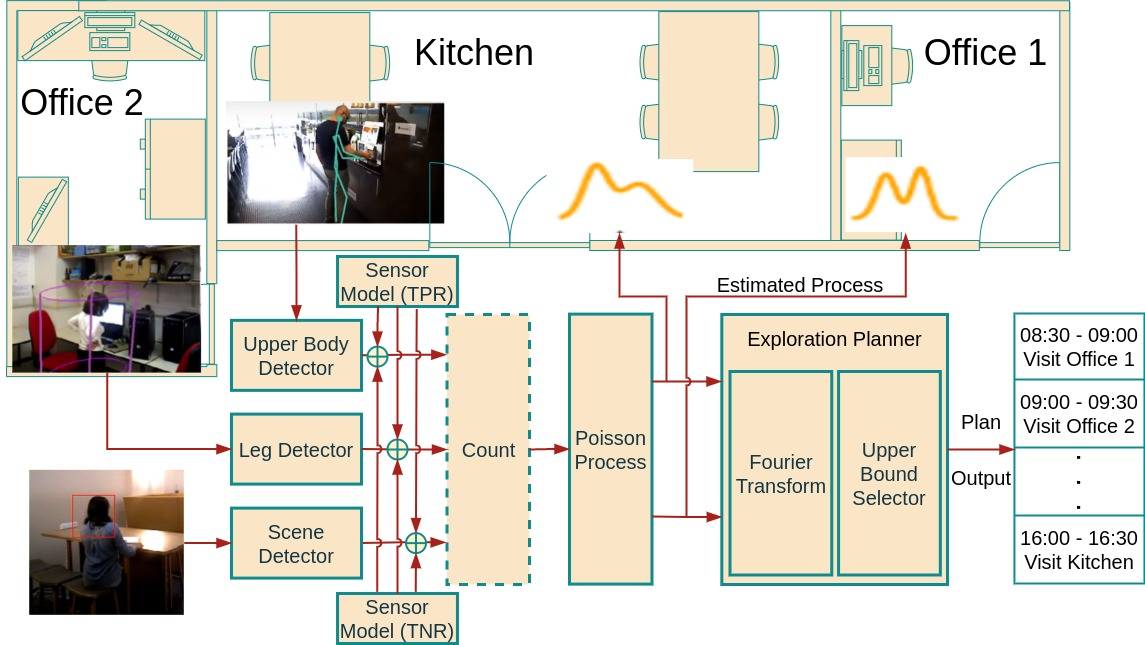
\includegraphics[width=0.8\textwidth]{./figures/popp_exploration_process.jpeg}
	\caption{A cycle process from count data collection, Poisson process estimation, through exploration plan generation for one day in an office-like environment. Count data are collected through perception algorithms or sensors while the robot patrols. The raw count data from multiple sensors are correctly filtered and merged via Bayesian inference taking into account the unreliability and correlation of each sensor to estimate the underlying Poisson process on each region of interest. Each estimate of the Poisson process is used by the exploration planner to find the maximum upper-bound of the Poisson process at each time interval and the corresponding region is chosen as a place to visit.} 
	\label{fig:popp_exploration_process_diagram}
	\vspace{-25pt}
\end{figure}
As requirements to employ the FOPP model are unlikely to be met, some existing works on statistical models propose a way to work with observation data that are not fully observable. In some literature, this is termed \emph{misclassified counts}. Misclassification happens when there are \emph{false positive counts} or \emph{false negative counts} (or both). False positive counts, also called the overcount, occur when the count includes events other than those of interest. False negative counts, also called the undercount, occur when some of the events of interest are missed. Work on the undercounting problem is common. Whittemore and Gong estimated cervical cancer rates by taking into account false negative data~\cite{whittemore1991}. Winkelmann and Zimmermann introduced a combination of a Poisson regression model with a logit model for under-counting, yielding the Poisson-Logistic (Pogit) model~\cite{winkelmann1993poisson}. They applied this to model the number of days employees were absent from a workplace. Dvorzak and Wagner adapted the Pogit model to use a small set of validation data, to provide information about the true counts~\cite{dvorzak2016}. They performed a Bayesian analysis of the Poisson-Logistic model and incorporate Bayesian variable selection to identify regressors with a non-zero effect and also to restrict parameters of the Poisson-Logistic model.

There is less prior work on the Poisson model for the case where the data may either be undercounted or overcounted~\cite{sposto1992,bratcher2002,bratcher2004,stamey2005}. Sposto et al. followed a frequentist approach to estimate both cancer and non-cancer death rates, assuming false negatives are possible on both sides of these counts~\cite{sposto1992}. In~\cite{bratcher2002}, Bratcher and Stamey used a Bayesian method to estimate Poisson rates in the presence of both undercounts and overcounts, borrowing the double sampling technique introduced in~\cite{Tenenbein1970}. They extended their work to a fully Bayesian method for interval prediction of the unobservable actual count in future samples, given a current double sample~\cite{bratcher2004}. Stamey and Young~\cite{stamey2005} present closed-form expressions for maximum likelihood estimators of the false negative rate, the false positive rate, and the Poisson rate for the model proposed in~\cite{bratcher2002}. The estimators are straightforward to calculate and to interpret in terms of evaluating the effectiveness of using unreliable counts.

Probabilistic approaches which do reason about sensing reliability have been applied to search and planning for robotics in a variety of settings. Many of them focus on optimization and maximization utilising the sensor model learned from observations in a continuous space. Velez et al. \cite{velez2012modelling} planned trajectories in a continuous space to maximize the reliability of object detection using a learned observation model. The key contribution is the use of a model of the correlations in sensor behaviour at nearby locations, thus driving the robot to gather more informative views. Martinez-Cantin et al. \cite{martinez2009bayesian} give a POMDP formulation of active visual mapping, use direct policy search to find a solution, and use Monte Carlo simulation to generate imaginary observations and action outcomes during optimization. The main challenge of decision-theoretic planning in partially observable environments is intractability. Kaplow et al. \cite{kaplow2010variable} employed a variable resolution map to achieve scaling with a robotic wheelchair. Task-level robot control with a decision-theoretic framework was first tackled by Pineau et al. \cite{pineau2003towards} using a POMDP planner to derive a high-level controller for a mobile robot with a dialogue system by exploiting hierarchy to reduce the state space.

What we propose is similar to that of Bratcher and Stamey~\cite{bratcher2002}. Both aim to accurately estimate the arrival rate parameter of a single Poisson process. Bratcher and Stamey utilise double sampling to obtain the true count together with false positive and false negative counts. They estimate the rate via MCMC since no closed form is found for $\lambda$, and the calculation of the full posterior is expensive. Double sampling assumes access to two counters with one always being a perfect counter. Our work goes beyond this since we consider multiple, potentially correlated, but always unreliable counters. We extend the work of Jovan et al in \cite{jovan18a} by presenting three extensions of our original model. We apply these extensions to the problem of robot exploration to optimize human robot-interactions. Similar to the work of Velez et al \cite{velez2012modelling} in utilizing sensor behaviours in driving the robot to gather more information, our work goes further by utilizing an exploration-exploitation mechanism provided by Bayesian optimization to maximize human interactions in the areas of interest.

% involved binomial and multinomial models~\cite{Bross1954,Chen1979,Hochberg1977,Tenenbein1970,Viana1993}. The first technique which was recorded to handle misclassification was double sampling. It was first introduced by Tenenbein to correct for misclassification of binomial data and obtain a maximum likelihood estimate~\cite{Tenenbein1970}. The double sampling approach utilizes two search techniques to retrieve relevant information: an expensive classification technique to obtain the true count along with the false positive count and false negative count from typically a small sample set, and a less-expensive classification technique only for error-prone counts on a larger sample set. The results of both counts are then combined to obtain estimators for the Poisson rate $\lambda$, and also for the misclassification parameters. The work of Tenenbein was then extended by Chen~\cite{Chen1979} and Hochberg~\cite{Hochberg1977} to correct misclassified counts in categorical and multinomial models to obtain maximum likelihood estimates. The double sampling technique was also extended to incorporate prior distributions in the binomial model and the posterior was obtained via Bayesian estimation~\cite{Viana1993}. Bekele extended the work of~\cite{Viana1993} by introducing a weighted prior scheme and allowing for several sources of information, including expert opinions~\cite{bekele1998binomial}.

% Different than the case of binomial and multinomial models, only a few studies are found working on the effect of partial observability of the data on the Poisson distribution. Many deal 

%!TEX root = ../bare_jrnl.tex

\section{Fully Observable Poisson Process}
\label{sec:preliminaries}

A \emph{fully observable} Poisson process (FOPP) models the distribution of $N(t)$, the number of events appearing in time interval $[0, t)$, parameterised by an \textit{arrival rate}, $\lambda$:
\begin{equation}
    \label{eq:pmf_poisson}
	Poi(N(t) = c \mid \lambda) = \frac{e ^{-\lambda} \lambda ^{c}}{c!}
\end{equation}
We use $N(t) = c_i$ to refer to a count recorded during the $i$-th observation of the process.
Given a Gamma density
\begin{equation}
    \label{eq:pdf_gamma}
    \begin{tabular}{rcl}
        $Gam(\lambda \mid \alpha, \beta)$ & = & $\displaystyle\frac{\beta ^{\alpha}}{\Gamma (\alpha)} \lambda ^{\alpha - 1} e^{-\beta \lambda}$ \\ [1ex]
    \end{tabular}
\end{equation}
as a prior distribution over the parameter $\lambda$, where $\alpha, \beta$ are the shape and the rate parameters, the posterior over $\lambda$ for a FOPP can be  calculated via Bayesian inference with
\begin{equation}
    \label{eq:posterior_fopp}
    \begin{array}{lll}
        P(\lambda \mid c_1, \ldots, c_n) & \varpropto Poi(c_1, \ldots, c_n \mid \lambda) ~ Gam(\lambda \mid \alpha, \beta) \\
         & = Gam \Bigg(\lambda \Bigm| \displaystyle\sum_{i=1}^{n} \alpha + c_i, \beta + n \Bigg)
    \end{array}
\end{equation}
This adds the sample counts $\sum_{i=1}^{n} c_i$ to the hyper-parameter $\alpha$ of the gamma prior, and adds the number of observations $n$ to the hyper-parameter $\beta$ of the gamma prior.

The FOPP model requires a single reliable sensor. With an unreliable sensor, FOPP inferences will be incorrect.
%!TEX root = ../sample.tex

\section{The Partially Observable Poisson Process}
\label{sec:popp}

The \emph{partially observable} Poisson process (POPP) is a counting process $N(t)$ with arrival rate $\lambda$ where the number of events appearing over the time interval $[0, t)$ is observed by one or more \emph{unreliable} counters. 
% 
The definition brings a distinction between the \emph{true count} (or simply \emph{count}), which refers to the number of events that actually occurred, and the \emph{sensed count}, which refers to the count obtained by a counter (or sensor). Let $c_i$ represent the true count over the interval $[0, t)$ during the $i$-th observation. With $m$ counters unreliably observing $c_i$, we use  $s_{j,i}$ to represent the sensed count given by sensor $j$ in the $i$-th observation within the interval $[0, t)$ with $1 \leq j \leq m$. Let $\mathbf{s_i} = (s_{1,i}, \ldots, s_{m,i})$ represent a vector of sensed counts from $m$ sensors for the $i$-th observation of the process. 

\begin{figure}[t!]
	\centering
	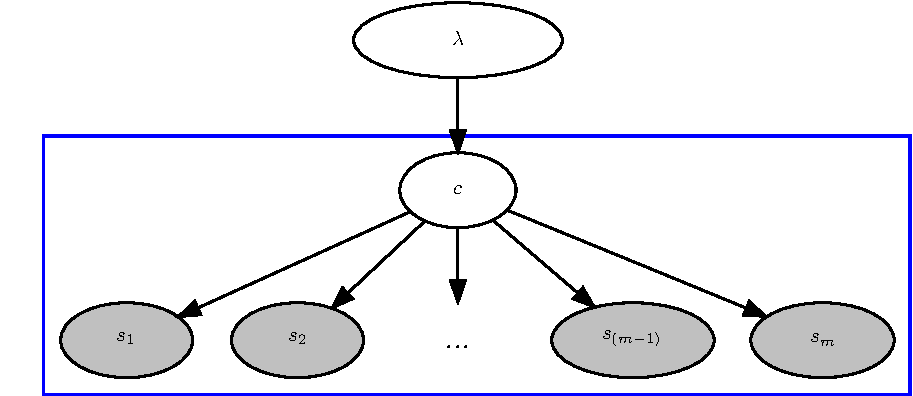
\includegraphics[width=0.75\textwidth]{./figures/popp-pics.pdf}
	\caption{Graphical representation of the partially observable Poisson process.}
	\label{fig:gm_popp}
	\vspace{-10pt}
\end{figure}

Figure~\ref{fig:gm_popp} presents the graphical model derived from the definition of the POPP. This shows that the true count $c_i$ has become a latent variable which can only be inferred from the sensed count.
% 
The posterior of $\lambda$ is then inferred from the posterior of $c_i$ after $n$ observations, $i = 1 \ldots n$. 
% \textbf{TODO: Fix figure to have \emph{multiple} $c_i$s not a single $X_i$. \emph{$c_i$ can not be multiple since it is the true count at time interval $i$, the sensed count can be multiple since they may come from different sensors.}	}

% The rate parameter $\lambda$ of the POPP model can be inferred by marginalising over all possible true count values $c_i$ in $P(\lambda \mid c_i)$ and in the  distribution of true counts given sensed counts $P(c_i \mid \mathbf{s_i})$. 
The rate parameter $\lambda$ of the POPP model can be inferred by marginalising over all possible true count values $c_i$ and in the  distribution of true counts given sensed counts $P(c_i \mid \mathbf{s_i})$.
% 
Given $n$ observations of the underlying process, let all observed true counts be represented by $\mathbf{c} = (c_1, \ldots, c_n)$, and all sensed counts by $\mathbf{s}=(\mathbf{s_1} \dots \mathbf{s_n})$, for $1 \leq i \leq n$ (recalling each $\mathbf{s_n}$ is produced by $m$ sensors). 
% 
The posterior of $\lambda$ is then:
\begin{equation}
	\label{eq:marginal_occurrences}
	\begin{tabular}{r@{=}l}
		$P(\lambda \mid \mathbf{s})$ &  $\displaystyle\sum_{c_1=0}^{\infty} \ldots \displaystyle\sum_{c_n=0}^{\infty} P(\lambda \mid \mathbf{c}) ~ P(\mathbf{c} \mid \mathbf{s})$ \\
	\end{tabular}
\end{equation}
\noindent where true count probabilities, $P(\lambda \mid \mathbf{c})$, can be drawn from the original FOPP definition:
\begin{equation}
	\label{eq:gamma_posterior_fopp}
	\begin{tabular}{r@{ = }l}
		$P(\lambda \mid \mathbf{c})$ & $Gam\Bigg(\lambda \Bigm| \displaystyle\sum_{i=1}^{n} c_i + \alpha, n + \beta \Bigg)$
	\end{tabular}
\end{equation}
If we assume that the sensor counts for observation period $i$ are conditionally independent (i.e.~\textit{uncorrelated}) given the true count $c_i$, then the probability of a collection of observations given the true count is defined as follows: 
\begin{equation}
	\label{eq:independent_sensor_likelihood}
	\begin{tabular}{r@{=}l}
		$P(\mathbf{s_i} \mid c_i)$ & $\displaystyle\prod_{j=1}^{m} P(s_{j,i} \mid c_i)$ \\ 
	\end{tabular}
\end{equation}
Using this, the probability of a particular sequence of $n$ counts, given a sequence of $n$ observations each from $m$ sensors, $P(\mathbf{c} \mid \mathbf{s})$, can be defined as:
\begin{equation}
	\label{eq:occurrences_likelihood}
	\begin{tabular}{r@{ $\varpropto$ }l}
		$P(\mathbf{c} \mid \mathbf{s})$ & $P(\mathbf{s_1}, \ldots, \mathbf{s_n} \mid \mathbf{c}) ~ P(\mathbf{c})$ \\ [1ex]
		& $\displaystyle\prod_{i=1}^{n} P(\mathbf{s_i} \mid c_i) ~ P(c_i \mid \mathbf{s_{i-1}}, \ldots, \mathbf{s_{1}})$ \\ [2ex]
		& $\displaystyle\prod_{i=1}^{n} \displaystyle\prod_{j=1}^{m} P(s_{j,i} \mid c_i) ~ P(c_i \mid \mathbf{s_{-1}})$
	\end{tabular}
\end{equation}
\noindent where $\mathbf{s_{-1}} = \mathbf{s_{i-1}}, \ldots, \mathbf{s_1}$\footnote{$s_{-1}$ does not exist whenever $i = 1$, and \\ $P(c_i) = \int_{\lambda=0}^{\infty} P(c_i \mid \lambda) ~ Gam(\lambda \mid \alpha, \beta) ~d\lambda$} and \hspace{0.3cm}$P(c_i \mid \mathbf{s_{-1}})$ can be calculated as:
% $P(c_i \mid \mathbf{c_{-1}})$ can be calculated using a negative binomial distribution:
\begin{equation}
	\label{eq:unconditional_xi}
	\begin{tabular}{r@{=}l}
		$P(c_i \mid \mathbf{s_{-1}})$ & $\displaystyle\int_{\lambda=0}^{\infty} P(c_i \mid \lambda) ~ P(\lambda \mid \mathbf{s_{-1}}) ~d\lambda$ \\ [2ex]
		%& $\displaystyle\int_{\lambda=0}^{\infty} Poi(c_i \mid \lambda) ~ Gam(\lambda \mid \alpha_{-1}, \beta_{-1}) ~d\lambda$ \\ [2ex]
		%& $NB\Bigg(c_i \Bigm| \alpha_{-1}, \displaystyle\frac{\beta_{-1}}{\beta_{-1} + 1}\Bigg)$.
	\end{tabular}
\end{equation}
% \noindent with $P(\lambda \mid \mathbf{c_{-1}})$ that does not follow \ref{eq:gamma_posterior_fopp} since the hyperparameters $\alpha_{-1}, \beta_{-1}$ in $Gam(\lambda \mid \alpha_{-1}, \beta_{-1})$ are not the original hyperparameters $\alpha, \beta$ as in \ref{eq:gamma_posterior_fopp}. The hyperparameters $\alpha_{-1}, \beta_{-1}$ are the hyperparameters obtained after $P(\lambda \mid s_1, \ldots, s_{i-1})$ has been calculated.
To complete Eq. \ref{eq:occurrences_likelihood} we must also define $P(s_{j,i} \mid c_i)$. The Poisson limit theorem states that the Poisson distribution may be used as an approximation to the binomial distribution \cite{papoulis2002probability}. Using this theorem as the foundation, an arbitrarily close approximation to the probability $P(s_{j,i} \mid c_i)$ is defined by assuming there exists a small enough finite subinterval of length $\delta$ for which the probability of more than one event occurring is less than some small value $ \epsilon$ and that $\delta$ is small enough that $\epsilon$ is negligible. With this assumption, interval $[0, t)$ is split into $l$ smaller subintervals $I_1, \ldots, I_l$ of equal size, with the condition that $l > \lambda$. Consequently, the whole interval $[0, t) = I_1, \ldots, I_l$ becomes a series of Bernoulli trials, where the $k^{th}$ trial corresponds to whether (1) an event $e_k$ happens with probability $\lambda / l$ and (2) a sensor $j$ captures the event $e_k$ as the detection $d_k$ at the subinterval $I_k$.

Following this, $P(s_{j,i} \mid c_i)$ can be defined using of the count of true  positives given $c_i$ subintervals, and the false positives given the remaining $l-c_i$ subintervals. 
% 
Let the probability of a \textit{true positive detection} (TP) for sensor $j$ in a single subinterval be $\tau_j=P_j(d \mid e{=}1)$, and the probability of a \textit{false positive detection} (FP) be $\xi_j = P_j(d \mid e{=}0)$. Thus $P(s_{j,i} \mid c_i)$ is defined as a sum over all possible sensed counts of the product of two binomial distributions $B(r \mid n,\pi)$: 
\begin{equation}
	\label{eq:joint_binomial_distribution}
	P(s_{j,i} \mid c_i) \! = \! \! \! \displaystyle\sum_{r = 0}^{c_{i}} \! \! B\Big(r \mid c_i, \tau_j\Big) B\Big((s_{j,i} - r) \mid (l - c_{i}), \xi_j \Big)
\end{equation}
\noindent where the first binomial provides the probability of getting some proportion of the count from  TP detections and the second binomial provides the probability of getting the remainder from FP detections. 

% \textbf{NOTE: This constraints $s_{j,i} \leq c_i$, doesn't it? Is it worth commenting on this? If we don't want this then we need to introduce $l$ a little more formally than was done before. \emph{we do not constraint it, $s_{j, i}$ can be greater than $c_i$. if $s_{j, i}$ is greater than $c_i$ it means that some portion of $s_{j, i}$ contains false positive.}}

Eq.~\ref{eq:marginal_occurrences} shows the difficulty of estimation in the POPP model. Since no conjugate density provides an analytical solution for the posterior over $\lambda$, every sensed count $\mathbf{s_i}$ must be retained to calculate the posterior of $\lambda$. That means elements representing each value of $c_i$ on each observation grow infinitely. Even with an upper bound $l$ on the maximum value of $c_i$, the number of elements to retain on each observation periods grows exponentially.

% Therefore each of the $n$ observation periods adds a factor of a countably infinite number of elements, and therefore the posterior is a sum of countably infinite sums. Even with an upper bound $l$ on the maximum value of $c_i$, the number of elements in the posterior grows by $l$ with each observation period.
% 
\subsection*{$\lambda$ Estimators}\label{sec:estimators}

To address this difficulty, in~\cite{jovan18a} we proposed three estimators, each of which offers an approximation to the true posterior $P(\lambda \mid \mathbf{s})$. The estimators are: \\
(1) a \textit{gamma filter}, which approximates Eq.~\ref{eq:marginal_occurrences} with a single gamma distribution minimising the KL-divergence $D_{KL}(P(\lambda \mid \mathbf{s}) \mid \mid Gam(\lambda \mid \alpha, \beta))$ by gradient descent. The accuracy of this filter deteriorates as sensor reliability degrades. However, computation time is constant on each observation and Eq. \ref{eq:unconditional_xi} has a closed form, using the negative binomial distribution
\begin{equation}
	\label{eq:unconditional_xi_gamma_filter}
	\begin{tabular}{r@{=}l}
		$P(c_i \mid \mathbf{s_{-1}})$ & $\displaystyle\int_{\lambda=0}^{\infty} P(c_i \mid \lambda) ~ P(\lambda \mid \mathbf{s_{-1}}) ~d\lambda$ \\ [2ex]
		& $\displaystyle\int_{\lambda=0}^{\infty} Poi(c_i \mid \lambda) ~ Gam(\lambda \mid \alpha_{-1}, \beta_{-1}) ~d\lambda$ \\ [2ex]
		& $NB\Bigg(c_i \Bigm| \alpha_{-1}, \displaystyle\frac{\beta_{-1}}{\beta_{-1} + 1}\Bigg)$.
	\end{tabular}
\end{equation}
\noindent with the hyperparameters $\alpha_{-1}, \beta_{-1}$ in $Gam(\lambda \mid \alpha_{-1}, \beta_{-1})$ being the updated hyperparameters obtained after $P(\lambda \mid s_1, \ldots, s_{i-1})$ has been calculated;\\
(2) a \textit{histogram filter}, which approximates Eq.~\ref{eq:marginal_occurrences} with a discrete distribution $Q(\lambda \mid \mathbf{s})$ by quantising $\lambda$. The advantage of this filter over the gamma filter is that it can track the posterior to an arbitrary fidelity via a finer quantisation with the cost of computation time. Its disadvantage is an increase in computation time compared to the gamma filter; \\
(3) a \textit{switching filter}, which approximates Eq.~\ref{eq:marginal_occurrences} either by a gamma filter or by a histogram filter depending on whether $P(\lambda \mid \mathbf{s})$  resembles a gamma distribution and can be approximated by the gamma filter via KL-divergence $D_{KL}(P(\lambda \mid \mathbf{s}) \mid \mid Gam(\lambda \mid \alpha, \beta))$.

\begin{figure}[t!]
	\centering
	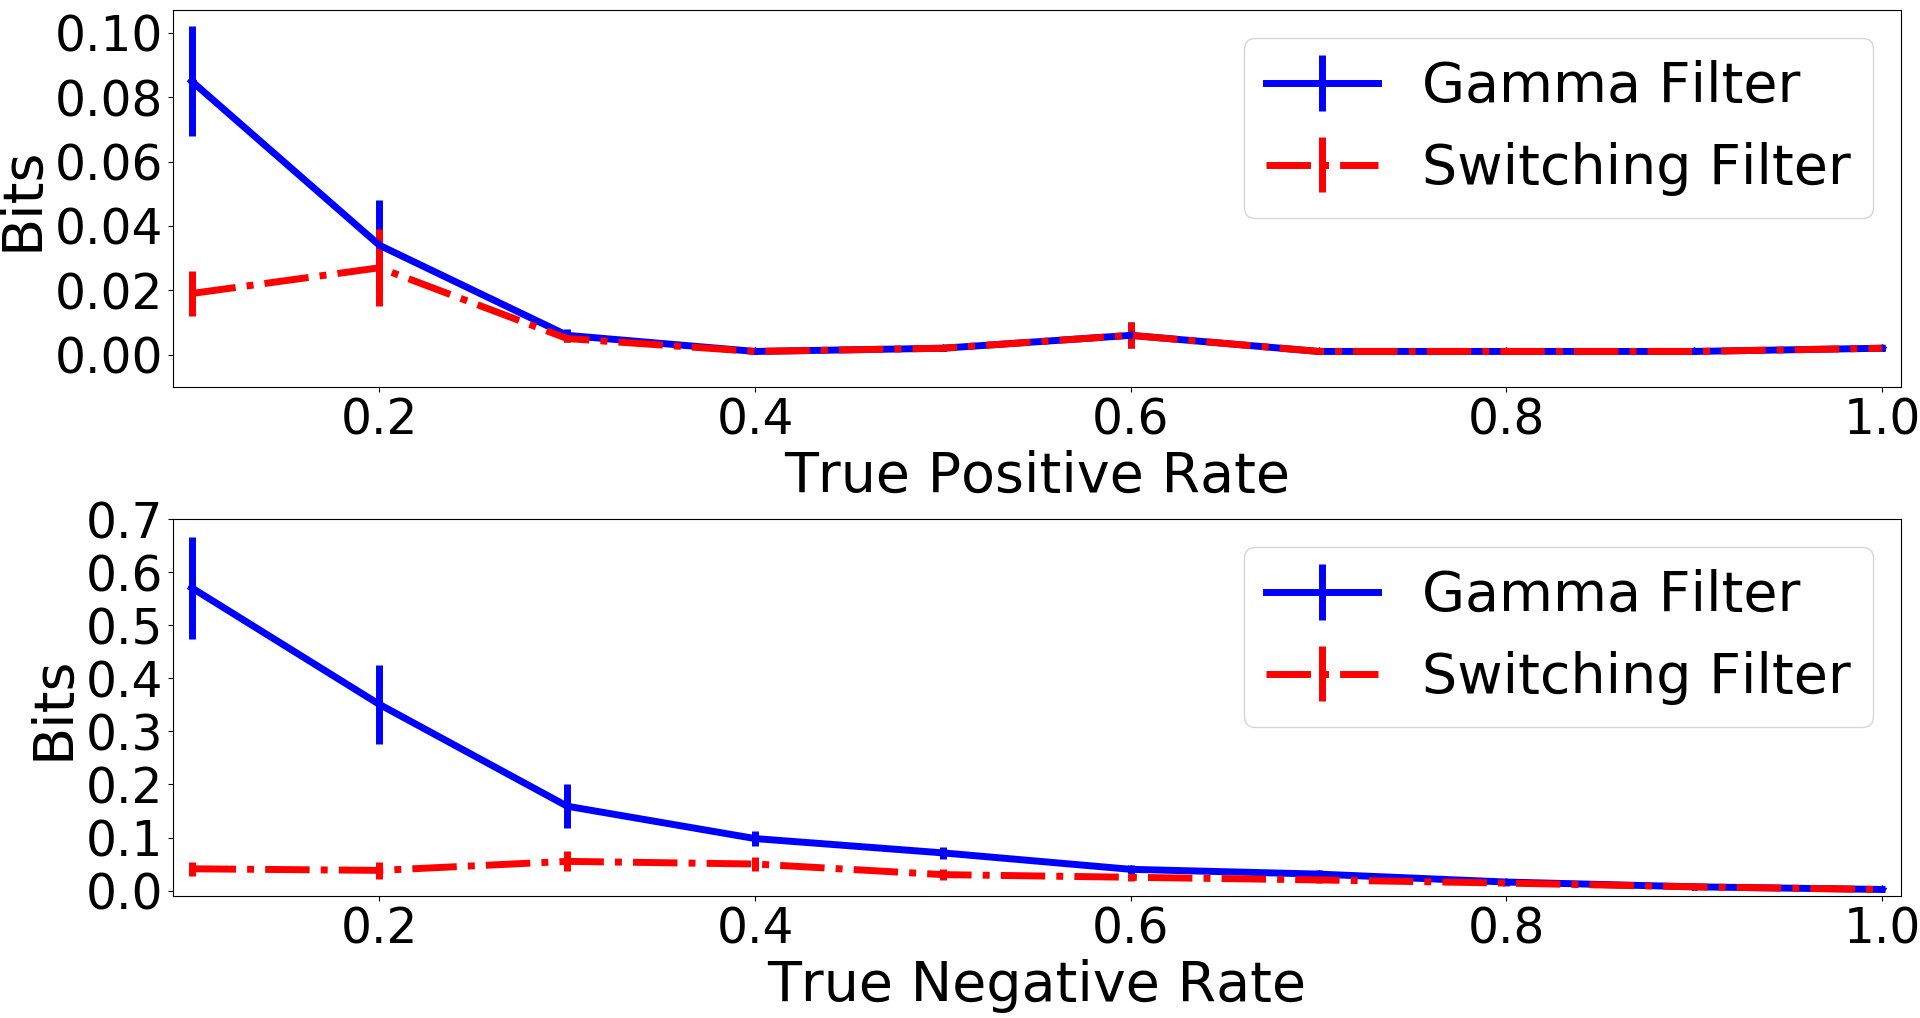
\includegraphics[width=0.75\textwidth]{./figures/kl_div_tpr_tnr_var.png}
	\caption{Average KL-divergence from the gamma and switching filters to $P(\lambda \mid \protect\mathbf{s})$. The horizontal axis shows the true positive rate (top) and true negative rate (bottom) of one simulated sensor. Standard error is shown.} 
	\label{fig:kl_div_tpr_tnr_var}
	\vspace{-20pt}
\end{figure}

In general (and in our experimental work from Section~\ref{sec:evasim} onwards) we use the switching filter as the estimator to the true posterior $P(\lambda \mid \mathbf{s})$ because it combines the best of both the gamma filter (fast calculation) and the histogram filter (accurate approximation) with minimum loss in similarity to the true posterior $P(\lambda \mid \mathbf{s})$. Figure \ref{fig:kl_div_tpr_tnr_var} shows KL-divergence between the gamma and switching filters to the true posterior over different sensor reliabilities using simulated data. Note that the histogram filter was not included because it perfectly tracked $P(\lambda \mid \mathbf{s})$, i.e., $D_{KL}(P(\lambda \mid \mathbf{s}) \mid \mid Q(\lambda \mid \mathbf{s})) \approx 0$. A more detailed presentation of these estimators is given in~\cite{jovan18a}.
% \input{src/filter.tex}
%!TEX root = ../sample.tex

\section{The POPP Extensions}
\label{sec:popp_extensions}

In~\cite{jovan18a} we demonstrated that the POPP model is able to efficiently correct miscounts made by multiple unreliable counting devices observing a single Poisson process. However, the POPP model is limited by two assumptions:
\begin{enumerate}
	\item the sensors are conditionally independent given the true count, and 
	\item the degree of the unreliability of a sensor (i.e. $\tau$ and $\xi$) is precisely known.
\end{enumerate}
In this paper, we propose three extensions to the POPP model to tackle these assumptions. The first extension (POPP-Beta) extends the POPP model with an observation model which captures uncertainty about the role of the sensor reliability. The second extension (C-POPP) modifies the POPP model to accommodate correlations between sensors. The third extension (POPP-Dirichlet) combines these ideas to jointly address both assumptions. 

\subsection{POPP-Beta}
\label{subsec:popb}

The POPP model requires the true positive and false positive rates to be specified for sensor $j$, i.e.  $\tau_j = P_j(d \mid e{=}1)$ and $\xi_j = P_j(d \mid e{=}0)$. 
The POPP model requires these rates to be accurate in order to generate correct posteriors over $\lambda$. To accurately determine the rates in practice, one needs to have a large data set of both sensed counts and the ground truth. Given the ground truth is typically manually created, this places a large burden on experts who need to label the data.   

Here, we extend the original POPP model to take into account uncertainty in the true and false positive rates due to limited training data.
% 
To model this uncertainty we use Bayesian estimation to determine the 
true positive rate ($\tau$) and false positive rate ($\xi$).
% 
We use Beta distributions as priors for $\tau$ and $\xi$ because the Beta distribution act as a conjugate to the binomial distribution, providing a family of prior probability distributions for the parameter of a binomial distribution. The Beta-binomial conjugacy leads to an analytically tractable compound distribution called the Beta-binomial distribution $BB(d \mid c, \zeta, \eta)$, where the $p$ parameter in the binomial distribution $B(d \mid c, p)$ is drawn from a Beta distribution $Be(p \mid \zeta, \eta)$.

\begin{figure}[t!]
	\centering
	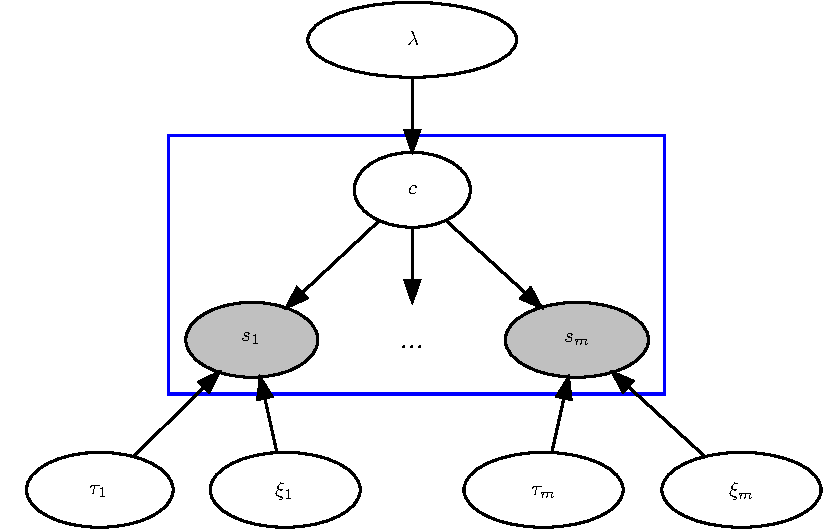
\includegraphics[width=0.75\textwidth]{./figures/popb-pics.pdf}
	\caption{Graphical representation of the POPP-Beta. Instead of having fixed estimated points for the sensor rates $\tau$ and $\xi$ like in the POPP model, they are represented by Beta distributions in the POPP-Beta.}
	\label{fig:gm_popb}
	\vspace{-20pt}
\end{figure}

% \begin{equation}
% 	\label{eq:beta_binomial}
% 	\begin{tabular}{r@{ = }l}
% 		$P(d ; c, \zeta, \eta)$ & $\displaystyle\int_{0}^{1} P(d ; c, p) ~ P(p ; \zeta, \eta) ~dp$ \\ [2ex]
% 		& $\displaystyle\int_{0}^{1} B(d ; c, p) ~ Be(p ; \zeta, \eta) ~dp$ \\ [2ex]
%         & $\displaystyle\int_{0}^{1} \binom{c}{d} p^d (1-p)^{(c-d)} ~ \displaystyle\frac{p^{(\zeta - 1)} (1-p)^{(\eta-1)}}{\pi(\zeta, \eta)}$ \\ [2ex]
%         & $\displaystyle\binom cd \displaystyle\frac{1}{\pi(\zeta, \eta)} \displaystyle\int_{0}^{1} p^{(d+\zeta-1)} (1-p)^{(c-d+\eta-1)} dp$ \\ [2ex]
%         & $\displaystyle\binom cd \displaystyle\frac{\pi(d+\zeta, c-d+\eta)}{\pi(\zeta, \eta)}$ \\ [2ex]
%         & $BB(d ; c, \zeta, \eta)$
% 	\end{tabular}
% \end{equation}

Our sensor rates, $\tau_j$ and $\xi_j$, are now estimated from two Beta distributions: $Be(\tau \mid \zeta_{\tau}, \eta_{\tau})$ and $Be(\xi \mid \zeta_{\xi}, \eta_{\xi})$.
% 
$\zeta_{\tau}$ and $\zeta_{\xi}$ are the number of true positive and false positive detections in the ground truth data respectively.
% 
$\eta_{\tau}$ and $\eta_{\xi}$ are the number of true negative and false  negative detections in the ground truth data respectively. 
% 
Given these parameters, we form the POPP-Beta model from POPP by replacing Eq. \ref{eq:joint_binomial_distribution} with:  

\begin{equation}
	\label{eq:joint_beta_binomial_distribution}
    P(s_{j,i} \mid c_i) \! = \! \! \! \displaystyle\sum_{r = 0}^{c_{i}} \! \! ~ BB\Big(r \Bigm| c_i, \zeta_{\tau}, \eta_{\tau} \Big) BB\Big( \delta_s r \Bigm| \delta_c r, \zeta_{\xi}, \eta_{\xi} \Big)
\end{equation}

\noindent with $\delta_s r = (s_{j,i} - r)$, and $\delta_c r = (l - c_i)$.

% With a sensor model which follows beta densities and is fully integrated, as a distribution, in the sensed count likelihood $P(s_{ji} ; c_i)$ as shown in Equation \ref{eq:joint_beta_binomial_distribution}, we obtain a graphical model with the structure shown in Figure \ref{fig:gm_popp_beta}.
One should note that the difference between the POPP and POPP-Beta model, lies only in the change from Eq. \ref{eq:joint_binomial_distribution} to \ref{eq:joint_beta_binomial_distribution}. However, given little training data for the observation model, the POPP-Beta model is expected to be more conservative in estimating the posterior $P(\lambda \mid \mathbf{s})$ over $\lambda$ than the POPP model. 

% \begin{figure*}[t!]
% 	\centering
% 	\begin{tikzpicture}
% 	\tikzstyle{place}=[rectangle,draw=blue,thick,minimum size=5 mm]
% 	\tikzstyle{empty}=[rectangle,draw=white,thick,minimum size=5 mm]
% 	\tikzstyle{every label}=[black]
% 	\begin{scope}
% 	\node[place](31)[xshift=0mm]{$S_{1i}$};
% 	\node[place](32)[right of=31, xshift=20mm]{$S_{2i}$};
% 	\node[place](33)[right of=32, xshift=20mm]{$\ldots$};
% 	\node[place](34)[right of=33, xshift=20mm]{$S_{(m-1)i}$};
% 	\node[place](35)[right of=34, xshift=22mm]{$S_{mi}$};
% 	\node[place](21)[above of=33]{$X_i$} edge[post](31) edge[post](32) edge[post](33) edge[post](34) edge[post](35);
% 	\node[place](11)[above of=21]{$\lambda$} edge[post](21);
%     \node[place](12)[right of=11, xshift=20mm]{$\textrm{tpr}_{(m-1)}, \textrm{xi}_{(m-1)}$} edge[post](34);
%     \node[place](13)[left of=11, xshift=-20mm]{$\textrm{tpr}_{2}, \textrm{xi}_{2}$} edge[post](32);
%     \node[place](14)[right of=12, xshift=22mm]{$\textrm{tpr}_{m}, \textrm{xi}_{m}$} edge[post](35);
%     \node[place](15)[left of=13, xshift=-20mm]{$\textrm{tpr}_{1}, \textrm{xi}_{1}$} edge[post](31);
% 	\node[empty](01)[above of=11]{};
%     \node[place](02)[above of=12]{$(\zeta, \eta)_{\textrm{tpr}}, (\zeta, \eta)_{\textrm{xi}}$} edge[post](12);
%     \node[place](03)[above of=13]{$(\zeta, \eta)_{\textrm{tpr}}, (\zeta, \eta)_{\textrm{xi}}$} edge[post](13);
%     \node[place](04)[above of=14]{$(\zeta, \eta)_{\textrm{tpr}}, (\zeta, \eta)_{\textrm{xi}}$} edge[post](14);
%     \node[place](05)[above of=15]{$(\zeta, \eta)_{\textrm{tpr}}, (\zeta, \eta)_{\textrm{xi}}$} edge[post](15);
% 	\end{scope}
% 	\end{tikzpicture}
%     \caption{Graphical representation of the POPP-Beta.}
% 	\label{fig:gm_popp_beta}
% \end{figure*}
%!TEX root = ../sample.tex

\subsection{Correlated POPP}
\label{subsec:cpop}

Recall that Eq.~\ref{eq:independent_sensor_likelihood} is defined under the assumption that each sensor count is conditionally independent from all the others given the true count. This assumption ignores the correlations between sensors. To introduce correlations between sensors we must alter Eq.~\ref{eq:independent_sensor_likelihood} and
Eq.~\ref{eq:joint_binomial_distribution} from the POPP model.

Recall that the probability of a particular sensed count given the true count $P(\mathbf{s_i} \mid c_i)$ was defined from the Poisson limit theorem as a sequence of Bernoulli trials over $l$ subintervals. With correlated sensors, the observation of an event $e_k$ in the $k^{th}$ trial no longer follows the Bernoulli distribution. Instead it follows the categorical distribution, where the $k^{th}$ trial corresponds to whether a particular combination of binary detections $d_{1,k}, \ldots, d_{m,k}$ happens in subinterval $I_k$. Therefore, we move our notation from using $s_{j, i}$ representing sensed counts for particular sensor $j$ independently at time interval $i$ to a matrix representing $m$ sensor detections together at time interval $i$. Formally, we replace Eq.~\ref{eq:independent_sensor_likelihood} and Eq.~\ref{eq:joint_binomial_distribution} with a probability of a series of detection outcomes given the true count $c_i$ at interval $i$ as the following.

We first define for some interval $i$, $l$ subintervals, and $m$ sensors, there is a binary matrix of detections $\mathbf{D^i}$ \footnote{We drop the ($i$) for all notations in this subsection as we will consider a single interval}. $\mathbf{D} \in \mathcal{D}^{m , l}$ the set of binary matrices of dimension $m \times l$. Each column $k$ of $\mathbf{D}$, we denote $\mathbf{D}_{:k} = \mathbf{d} = \{0, 1\}^m$ with $k = 1, \ldots, l$. $\mathbf{D_{:k}}$ is a vector of detections from $m$ different sensors at particular subinterval $k$. 

We further define $e_k \in \{0, 1\}$ as the variable indicating whether or not an event is hypothesized to have occurred in sub-interval $k$. $e_k = 1$ means that an event occurred. We define $P^{+}$ as the categorical distribution of $\mathbf{d}$, conditioned on $e = 1$, i.e.
\begin{equation}
	\label{eq:joint_sensor_model_positive_event}
	P^+(\mathbf{d}) = P(\mathbf{d} \mid e = 1) ~~~~~ \forall \mathbf{d} \in \{0, 1\}^m
\end{equation} 
\noindent and, by analogy,
\begin{equation}
	\label{eq:joint_sensor_model_negative_event}
	P^-(\mathbf{d}) = P(\mathbf{d} \mid e = 0) ~~~~~ \forall \mathbf{d} \in \{0, 1\}^m
\end{equation}
\noindent Both $P^+$ and $P^-$ have $2^m$ elements\footnote{$\mathbf d$ is dropped in the representation unless the context is not clear.}. These two probabilities represent \textit{true positive rates} and \textit{true negative rates}  as $\tau$ and $\xi$ for the POPP model. Similar to $\tau$ and $\xi$, $P^+$ and $P^-$ are estimated from both detections of each sensor and the corresponding actual (non-)event as ground truth. However, unlike $\tau$ and $\xi$ which are sensor specific, $P^+$ and $P^-$ consider all combinations of binary detections from sensors given the true event. This means the number of elements in $P^+$ and $P^-$ grows by a factor of two for each sensor added. Due to the size of $P^+$ and $P^-$, they may need more than a few hundred of detections together with their corresponding events to be estimated.

We can partition the subintervals $1, \ldots, l$ into two sets. $\mathbf{e}^+$ is the set of subintervals $k$ where $e_k = 1$, and $\mathbf{e}^-$ is the set of subintervals $k$ where $e_k = 0$. We can define a partition of the subintervals by a pair $(\mathbf{e}^+, \mathbf{e}^-)$. The set of possible partitions such that $\mathbf{e}^+$ has a fixed size $c$, i.e. $\mid \mathbf{e}^+ \mid = c$, is denoted $\Sigma_c$, so that $(\mathbf{e}^+, \mathbf{e}^-) \in \Sigma_c$.

We further define $\mathbf{D}_{\mathbf{e}^+}$ as an $m \times c$ detection matrix formed from all the columns $\mathbf{D}_{:k}$ where $k \in \mathbf{e}^+$, and $\mathbf{D}_{\mathbf{e}^-}$ as the corresponding $m \times (l - c)$ detection matrix formed from all the columns $\mathbf{D}_{:k}$ where $k \in \mathbf{e}^-$.

As there may be duplicate columns in either or both $\mathbf{D}_{\mathbf{e}^+}$ and $\mathbf{D}_{\mathbf{e}^-}$, we define a count vector for each.
\begin{equation*}
	\mathbf{g}^+ = \textrm{count}(D_{\mathbf{e}^+})
\end{equation*}
\noindent and
\begin{equation*}
	\mathbf{g}^- = \textrm{count}(D_{\mathbf{e}^-})
\end{equation*}
\noindent such that $\sum\limits_{q=1}^{2^m} g_q^+ + \sum\limits_{r=1}^{2^m} g_r^- = l$ where each of $\mathbf{g}^+, \mathbf{g}^-$ are of length $2^m$, having one element for every possible detection vector $\mathbf{d} \in \{0, 1\}^m$.

\begin{figure}[t!]
	\centering
	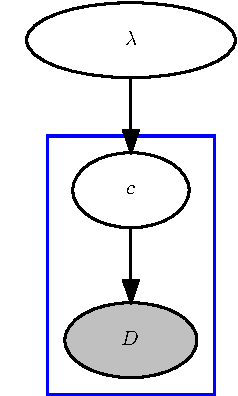
\includegraphics[width=0.2\textwidth]{./figures/cpop-pics.pdf}
	\caption{Graphical representation of C-POPP. Unlike the POPP model, the matrix detection $\mathbf{D}$ represents a joint detection at particular time interval and is affected by the value of the true count $c$, and the sensor rates (joint true positive rate $P^+$ and joint true negative rate $P^-$).} %Furthermore, similar to the POPP-Beta model, the sensor rates are represented by Dirichlet distributions.}
	\label{fig:gm_cpopp}
	\vspace{-20pt}
\end{figure}

In order to define the joint probability of a particular count being yielded by a particular sequence of detection outcomes, we must consider all possible combinations of true positives and false positives that could be generated by that sequence by exploring all elements of $\Sigma_c$. We do this in the following definition of $P(\mathbf{D} | c)$, and define the probability of a given sequence of detection groups yielding count $c$ using the multinomial distribution.
\begin{equation}
\label{eq:codependent_sensor_likelihood}
P(\mathbf{D} \mid c) = \sum\limits_{(\mathbf{e}^+, \mathbf{e}^-) \in \Sigma_c} Mult(\mathbf{g}^+ \mid c, P^+) ~ Mult(\mathbf{g}^- \mid \delta_l c, P^-)
\end{equation}
\noindent with $\delta_l c = (l - c)$.

Eq.~\ref{eq:codependent_sensor_likelihood} can be understood by analogy to Eq.~\ref{eq:joint_binomial_distribution}. In both equations all possible ways pairs of true and false positives counts which sum to $c$ are considered. In the conditionally independent case the binomial distribution is used to determine the probability of each count from the available trials given the true and false positive rates. However, in the conditionally independent case, Eq.~\ref{eq:joint_binomial_distribution} is calculated independently for each sensor, and the joint probability of those sensors results in Eq.~\ref{eq:independent_sensor_likelihood}. In the correlated case the multinomial distribution is used to determine the probability of each count from a possible sequence of joint observations and their probability of yielding a count. With that, Eq.\ref{eq:codependent_sensor_likelihood} removes the need of Eq.~\ref{eq:independent_sensor_likelihood} in C-POPP model. A graphical representation for C-POPP can be seen in Figure \ref{fig:gm_cpopp}.

One should note that the benefit of C-POPP is that it exploits correlations among multiple sensors contributing to detection counts. If there is only one sensor counting events, then C-POPP collapses to POPP.


%\subsection{The Correlated POPP}
%\label{subsec:cpop}
%
%Recall that Eq.~\ref{eq:occurrences_likelihood} is defined under the assumption that each sensor count is conditionally independent from all the others given the true count. This assumption ignores the correlations between sensors. 
%% 
%To introduce correlations between sensors we must alter Eq.~\ref{eq:independent_sensor_likelihood} and
%Eq.~\ref{eq:joint_binomial_distribution} from the POPP model.
%
%
%To replace Eq.~\ref{eq:joint_binomial_distribution}, recall that the probability of a particular sensed count was defined from the Poisson limit theorem as a sequence of Bernoulli trials over $l$ subintervals.
%% 
%With correlated sensors, the observation of an event $e_k$ in the 
%$k^{th}$ trial no longer follows the Bernoulli distribution. Instead it follows the categorical distribution, where the $k^{th}$ trial corresponds to whether a particular combination of binary detections $d_{1,k}, \ldots, d_{m,k}$ happens in subinterval $I_k$. Therefore, instead of having independent sensor models for the detection of event $e_k$ we propose the joint observation model:
%\begin{equation}
%\label{eq:joint_sensor_model}
%P_{jnt}(\mathbf{d_k} ; e_k)
%\end{equation}    
%\noindent where $ \mathbf{d_k} = (d_{1,k}, \ldots, d_{m,k})$, with $d_{j,k}$ being a detection by sensor $j$ in the $k^{th}$ subinterval, and $d_{j,k}, e_k \in {0, 1}$. 
%
%From this we define functions $\mathcal E^+, \mathcal E^- : \mathbf{d} \rightarrow [0,1]$ which provide the probability of a joint observation given that $e_k$ occurred or did not, respectively. 
%
%\begin{equation}
%\mathcal E^+ = P_{jnt}(\mathbf{d_k} ; e_k=1)
%\end{equation}
%\begin{equation}
%\mathcal E^- = P_{jnt}(\mathbf{d_k} ; e_k=0)
%\end{equation}
%
%
%% \textbf{NOTE: Probably not needed but this implies that the value of each function over all $\mathbf{d_k}$ sums to 1. \emph{$\mathcal E^+$ and $\mathcal E^-$, each sums up to 1. These $\mathcal E^+$ and $\mathcal E^-$ are basically the TPR and TNR in these joint observation/sensor models}}
%
%Recall that the set of detections for observation period $i$ was defined as:
%\begin{equation*}
%\mathbf{s_i} = (s_{1i}, \ldots, s_{mi})
%\end{equation*}
%with $s_{j,i} \in \mathbb N$, the sensed count of sensor $j$ from the $i$-th observation period. Since the joint observation model is defined under a combination of binary detections of sensors, each $s_{j,i}$ can be split into $l$ subintervals such that in each sub interval $I_k$ there is only one detection $d_{j,k}$. If the binary detections from all sensors at subinterval $I_k$ are grouped together, then for the observation period $i$, $\mathbf{s_i}$ can be alternatively defined as a list of $l$ \emph{detection groups} of binary detections:
%\begin{equation}
%\label{eq:s_i_definition}
%\mathbf{s'_i} = ((d_{1,1}, \ldots, d_{m,1}), \ldots, (d_{1,l}, \ldots, d_{m,l}))
%\end{equation}
%\noindent with $d_{j,k}$ being a detection by sensor $j$ at subinterval $I_k$ and $d_{j,k} \in \{0, 1\}$. 
%% Note that this is not a set since detection groups can be duplicated across subintervals.
%
%In order to define the joint probability of a particular count being yielded by a particular sequence of detection groups, we must consider all possible combinations of true positives and false positives that could be generated by that sequence. We do this in the following definition of $P(\mathbf{s_i} ; c_i)$, and define the probability of a given sequence of detection groups yielding count $c_i$ using the multinomial distribution.
%
%\begin{equation}
%\label{eq:codependent_sensor_likelihood}
%P(\mathbf{s_i} ; c_i) = \sum\limits_{\mathbf{s} \in \mathcal{P}(\mathbf{s'_i})} Multi(\mathbf{s} ; |\mathbf{s}|, \mathcal E^+) ~ Multi(\mathbf{s'_i}\setminus \mathbf{s} ; (c_i - |\mathbf{s}|), \mathcal E^-)
%\end{equation}
%
%\noindent where $\mathcal{P}(\mathbf{s'_i}) = 2^{\mathbf{s'_i}}$, i.e. the list all possible combinations of size $n$ from of elements of $s'_i$\footnote{We have used the powerset symbol, $\mathcal{P}$, since it provides an indication of the entity being created. However note that we are not working with sets since $\mathbf{s'_i}$ can contain multiple identical sequences of $d_{j,k}$.}. 
%
%% \textbf{NOTE: \emph{Is using powerset correct? How do we distinguish the total number of each $(d_{1,1}, \ldots, d_{m,1}$?}}
%
%Eq.~\ref{eq:codependent_sensor_likelihood} can be understood by analogy to Eq.~\ref{eq:joint_binomial_distribution}. In both equations all possible ways pairs of true and false positives counts which sum to $c_i$ are considered. In the conditionally independent case the binomial distribution is used to determine the probability of each count from the available trials given the true and false positive rates. In the correlated case the multinomial distribution is used to determine the probability of each count from a possible sequence of joint observations and their probability of yielding a count.
%
%One should note that the benefit of C-POPP is that it exploits correlations among multiple sensors contributing to detection counts. If there is only one sensor counting events, then the POPP model is more computationally efficient.

%!TEX root = ../sample.tex

\subsection{The POPP-Dirichlet}
\label{subsec:popd}

The C-POPP model requires the true positive rate $P^+$ and true negative rate $P^-$ to be specified in advanced in estimating the parameter $\lambda$ of a Poisson process. These are an extension of $\tau$ and $\xi$ where the rates provide a probability for a particular combination of binary detections coming from each sensor given the true event as shown in Eq. \ref{eq:joint_sensor_model_positive_event} and Eq. \ref{eq:joint_sensor_model_negative_event}.

To construct an observation model of $P^+$ and $P^-$, one needs to have both detections and the corresponding actual (non-)events as ground truth. Pre-processing involving expert interventions is typically required before the detections and their corresponding ground truth can be further used. Similarly to the POPP model, the C-POPP model requires the observation model to be accurate to avoid the posterior over $\lambda$ drifting away from the true posterior. If attaining an accurate observation model for the POPP model is a problem, then this becomes more challenging in the case of C-POPP model. This is because the training data needed to construct an observation model grows by a factor of two for each sensor involved.       

Analogously to the extension from the POPP model to the POPP-Beta model, we can expand the C-POPP observation model. In this case the observation models ($P^+$ and $P^-$) will follow Dirichlet distributions. The Dirichlet distribution is an appropriate distribution since $P^+$ and $P^-$ are the probabilities of categorical distributions which set the probabilities of multinomial distributions in Eq. \ref{eq:codependent_sensor_likelihood} and Dirichlet distributions provide a family of conjugate prior probability distributions for the multinomial distribution. The Dirichlet-multinomial conjugacy leads to an analytically tractable compound distribution which is called the Dirichlet-multinomial distribution, where the $\mathbf{p} = (p_1, \ldots, p_r)$ parameter in the multinomial distribution $Mult(\mathbf{d} \mid c, \mathbf{p})$ is randomly drawn from a Dirichlet distribution $Dir(\mathbf{p} \mid \boldsymbol{\zeta})$. 
\begin{equation}
	\label{eq:beta_binomial_revisit}
	\begin{tabular}{r@{ = }l}
        $P(\mathbf{d} \mid c, \boldsymbol{\zeta})$ & $\displaystyle\int P(\mathbf{d} \mid c, \mathbf{p}) ~ P(\mathbf{p} \mid \boldsymbol{\zeta}) ~d\mathbb S_r$ \\ [2ex]
        & $\displaystyle\int Mult(\mathbf{d} \mid c, \mathbf{p}) ~ Dir(\mathbf{p} \mid \boldsymbol{\zeta}) ~d\mathbb S_r$ \\ [2ex]
        & $DM((d_1, \ldots, d_r) \mid c, (\zeta_1, \ldots, \zeta_r))$
	\end{tabular}
\end{equation}
\noindent with $\mathbf{d} = (d_1, \ldots, d_r)$, $\boldsymbol{\zeta} = (\zeta_1, \ldots, \zeta_r)$, and $d\mathbb S_r$ denotes integrating $\mathbf{p}$ with respect to the $(r - 1)$ simplex\footnote{The support of the Dirichlet distribution is the $(r - 1)$-dimensional simplex $\mathbb S_r$; that is, all $r$ dimensional vectors which form a valid probability distribution}.

\begin{figure}[t!]
	\centering
	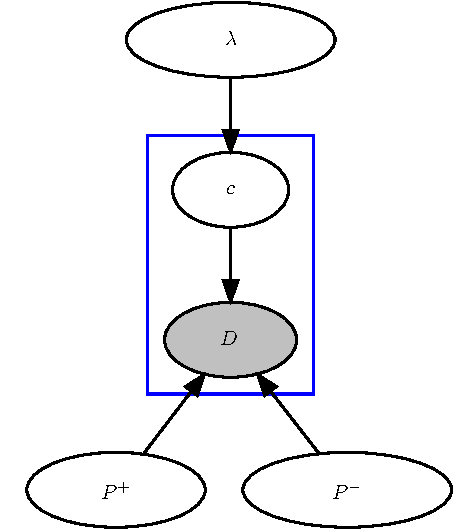
\includegraphics[width=0.35\textwidth]{./figures/popd-pics.pdf}
	\caption{Graphical representation of POPP-Dirichlet. Instead of having fixed estimated points for the (joint) sensor rates $P^+$ and $P^-$, they are represented by Dirichlet distributions in the POPP-Dirichlet.}
	\label{fig:gm_popp_dir}
	\vspace{-20pt}
\end{figure}

Given $m$ sensors, an observation model is now represented as two Dirichlet distributions: $Dir(P^+ \mid \boldsymbol{\zeta^+})$, and $Dir(P^- \mid \boldsymbol{\zeta^-})$ with $\boldsymbol{\zeta^+} = (\zeta^+_0, \ldots, \zeta^+_{(m^2)-1})$ and $\boldsymbol{\zeta^-} = (\zeta^-_0, \ldots, \zeta^-_{(m^2)-1})$. $\boldsymbol{\zeta^+}$ and $\boldsymbol{\zeta^-}$ set the overall shape of the Dirichlet priors, with each $\zeta_q$ term counting the number of times that particular combination of sensor detections were produced given a positive ($\boldsymbol{\zeta^+}$, $e=1$) or negative ($\boldsymbol{\zeta^-}$, $e=0$) detection.

Given a joint sensor model where its elements follow a Dirichlet density and several Dirichlet-multinomial distributions, which provide an unconditional distribution of $\mathbf{d}$, we replace Eq. \ref{eq:codependent_sensor_likelihood} with:  
\begin{equation}
	\label{eq:joint_dirichlet_multinomial_distribution}
    \begin{tabular}{r@{=}l}
		$P(\mathbf{D} \mid c)$ & $\sum\limits_{(\mathbf{e}^+, \mathbf{e}^-) \in \Sigma_c} DM(\mathbf{g}^+ \mid c, \boldsymbol{\zeta^+}) ~ DM(\mathbf{g}^- \mid (l - c), \boldsymbol{\zeta^-})$
	\end{tabular}
\end{equation}
\noindent with $\Sigma_c$ and $\mathbf{D}$ as defined in Section~\ref{subsec:cpop}.
% With a joint sensor model following the Dirichlet density, which is conjugated with multinomial distributions into a posterior predictive distribution shown in Eq. \ref{eq:joint_dirichlet_multinomial_distribution}, a graphical model is shown in Figure \ref{fig:gm_popp_dirichlet}.

The difference between the C-POPP model and the POPP-Dirichlet lies only in Eq. \ref{eq:codependent_sensor_likelihood} being replaced by \ref{eq:joint_dirichlet_multinomial_distribution} which is depicted by Figure \ref{fig:gm_popp_dir}. The difference makes the POPP-Dirichlet to be more conservative in estimating the posterior $P(\lambda \mid \mathbf{s})$ over $\lambda$ than the C-POPP model given a certain Dirichlet prior, and limited training data for the sensor model.

% \begin{figure}[t!]
% 	\centering
% 	\begin{tikzpicture}
% 	\tikzstyle{place}=[rectangle,draw=blue,thick,minimum size=5 mm]
% 	\tikzstyle{every label}=[black]
% 	\begin{scope}
%     \node[place](51)[xshift=30mm]{$(\zeta^+_0, \ldots, \zeta^+_{(m^2)-1})$};
%     \node[place](52)[right of=51, xshift=30mm]{$(\zeta^-_0, \ldots, \zeta^-_{(m^2)-1})$};
%     \node[place](41)[above of=51, yshift=3mm]{$(E^+_0, \ldots, E^+_{(m^2)-1})$} edge[pre](51);
%     \node[place](42)[above of=52, yshift=3mm]{$(E^-_0, \ldots, E^-_{(m^2)-1})$} edge[pre](52);
%     \node[place](31)[above of=41, xshift=-30mm, yshift=3mm]{$S_{1i}$} edge[pre](41) edge[pre](42);
% 	\node[place](32)[right of=31, xshift=20mm]{$S_{2i}$} edge[pre](41) edge[pre](42);
% 	\node[place](33)[right of=32, xshift=10mm]{$\ldots$} edge[pre](41) edge[pre](42);
% 	\node[place](34)[right of=33, xshift=15mm]{$S_{(m-1)i}$} edge[pre](41) edge[pre](42);
% 	\node[place](35)[right of=34, xshift=22mm]{$S_{mi}$} edge[pre](41) edge[pre](42);
% 	\node[place](21)[above of=33]{$X_i$} edge[post](31) edge[post](32) edge[post](33) edge[post](34) edge[post](35);
% 	\node[place](11)[above of=21]{$\lambda$} edge[post](21);
% 	% \node[place](01)[above of=11]{$\alpha, \beta$} edge[post](11);
% 	\end{scope}
% 	\end{tikzpicture}
% 	\caption{Graphical representation of the POPP-Dirichlet.}
% 	\label{fig:gm_popp_dirichlet}
% \end{figure}
%!TEX root = ../sample.tex

\section{Evaluation on Synthetic Data}
\label{sec:evasim}

In this section we evaluate POPP and its extensions on synthetic data to demonstrate the properties of these models when estimating the arrival rate $\lambda$ of a Poisson process. With synthetic data, sensor reliability can be controlled, and the true $\lambda$ and the true counts $c_i$ can be known for each sample.

% Here, an evaluation and a comparison of the POPP models to the FOPP model are conducted with two imaginary unreliable sensors and simulated datasets. The switching filter is chosen as a filter for all POPP models for this evaluation. 

In our experiments, we initially generate $n=12$ (true) counts from a Poisson process $P(c \mid \lambda'=3)$ with a time interval $t = 10$ time unit as a training set. Along with the counts $c_1, \ldots, \c_{12}$, for each count $c_i$, we also generate the corresponding event occurrence $e_k \in \{0, 1\}$ for $k \in \{1, \ldots, t\}$, and the matrix detection $\protect\mathbf{D_i}$ for two unreliable sensors (i.e. $m=2, l=10, \mathbf{D} \in \mathcal D^{2, 10}$ in our evaluation). To capture a range of possible sensor correlations and performance characteristics, a set of matrix detection $\protect\mathbf{D_1}, \ldots, \protect\mathbf{D_{12}}$ are produced from 12 different sensor configurations (see Table \ref{tab:eval_sim}).

In our experiments we initially generate a training set of $n=12$ (true) counts from a Poisson process $P(c \mid \lambda'=3)$ with a time interval $t = 10$ time unit. Along with the training set count $c_1, \ldots, c_{12}$, for each count $c_i$, we also generate the corresponding event occurrence $e_k \in \{0, 1\}$ on each subinterval $k \in \{1, \ldots, t\}$, a sensed count $\protect\mathbf{s_i}$, and $\protect\mathbf{D_i}$ from two unreliable sensors with 10 subintervals for each sensed count $\protect\mathbf{D_i}$ (i.e. $m=2, l=10, \mathbf{D} \in \mathcal D^{2, 10}$ in our evaluation). To capture a range of possible sensor correlations and performance characteristics, the sensed counts for the training set are produced from 12 different sensor configurations (see Table \ref{tab:eval_sim}). The true and sensed counts are then used to build (joint where appropriate) sensor models for the POPP extensions described above. For the POPP-Beta and the POPP-Dirichlet models, we set the hyperparameters of the Dirichlet prior and Beta prior to follow uniform distribution, i.e., $\zeta_{\tau} = \eta_{\tau} = \zeta_{\xi} = \eta_{\xi} = 1$ for the POPP-Beta, and $\boldsymbol{\zeta^+} = \boldsymbol{\zeta^-} = (1, 1, 1, 1)$ for the POPP-Dirichlet. Most of these (hyper) parameters ($l, t, \zeta, \eta, \boldsymbol{\zeta^+}, \boldsymbol{\zeta^-}$), except the number of sensors $m$, are reused in our real-world experiment in the next chapter.

We then generate a new set of $n=144$ true counts and the corresponding sensed counts for each of the 12 sensor configurations. These sensing are used as input in a filtering process to estimate the posterior of $\lambda$ according to each of the four models defined above (POPP, POPP-Beta, C-POPP, and POPP-Dirichlet), plus FOPP.
% 
We chose the training set size $n=12$ such that there is insufficient data to build an accurate sensor model. This allows the POPP-Dirichlet and the POPP-Beta models to compensate with loose Dirichlet and beta densities. 

The 12 sensor configurations mentioned previously represent 12 different experimental conditions under which we can test our proposed models. In six of the configurations we vary the true joint positive rates (true $P^+$) of the two sensors whilst fixing their true joint negative rates (true $P^-$). In the other six we fix the true joint positive rates (TJPRs) whilst varying the true joint negative rates (TJNRs). Both cases cover variations where the sensors are uncorrelated, positively correlated and negatively correlated, and in each case where the overall true (postive or negative) rates are either high (0.9) or low (0.1). The detailed configurations are presented in Table~\ref{tab:eval_sim}. 

\begin{table*}
\begin{center}
 \begin{tabular}{| c | c || c | c | c | c || c | c | c | c|} 
 \hline
     & $e_k$ &  \multicolumn{4}{|c||}{1} &  \multicolumn{4}{c|}{0} \\
 \hline
 & $d_{1,k}, d_{2,k}$  & 0, 0 & 0, 1 & 1, 0 & 1, 1 & 0, 0 & 0, 1 & 1, 0  & 1, 1\\  
 \hline\hline
 \textbf{TJPR} & \textbf{TJNR} &  &  &  &  &  &  &  & \\  
 \hline
 \hline
 low + corr & fixed & 0.1 & 0.0 & 0.0 & 0.9 & 1.0 & 0.0 & 0.0 & 0.0\\  
 \hline
 high + corr & fixed & 0.9 & 0.0 & 0.0 & 0.1 & 1.0 & 0.0 & 0.0 & 0.0\\  
 \hline
 low - corr & fixed & 0.0 & 0.05 & 0.05 & 0.9 & 1.0 & 0.0 & 0.0 & 0.0\\  
 \hline
 high - corr & fixed & 0.0 & 0.45 & 0.45 & 0.1 & 1.0 & 0.0 & 0.0 & 0.0\\  
 \hline
 no correlation & fixed & 0.033 & 0.033 & 0.033 & 0.901 & 1.0 & 0.0 & 0.0 & 0.0\\  
 \hline
 no correlation & fixed & 0.3 & 0.3 & 0.3 & 0.1 & 1.0 & 0.0 & 0.0 & 0.0\\  
 \hline
 fixed & low + corr  & 0.0 & 0.0 & 0.0 & 1.0 & 0.9 & 0.0 & 0.0 & 0.1\\  
 \hline
 fixed & high + corr  & 0.0 & 0.0 & 0.0 & 1.0 & 0.1 & 0.0 & 0.0 & 0.9\\  
 \hline
 fixed & low - corr  & 0.0 & 0.0 & 0.0 & 1.0 & 0.9 & 0.05 & 0.05 & 0.0\\  
 \hline
 fixed & high - corr  & 0.0 & 0.0 & 0.0 & 1.0 & 0.1 & 0.45 & 0.45 & 0.0\\  
 \hline
 fixed & no correlation  & 0.0 & 0.0 & 0.0 & 1.0 & 0.9 & 0.033 & 0.033 & 0.033\\  
 \hline
 fixed & no correlation  & 0.0 & 0.0 & 0.0 & 1.0 & 0.1 & 0.3 & 0.3 & 0.3\\  
 \hline
\end{tabular}
\end{center}
\vspace{-13pt}
\caption{The sensor configurations for the evaluation on synthetic data. "+ corr" and "- corr" mean a positive correlation and a negative correlation between two sensors respectively.}
\label{tab:eval_sim}
\vspace{-15pt}
\end{table*}


\begin{figure}[t!]
	\centering
	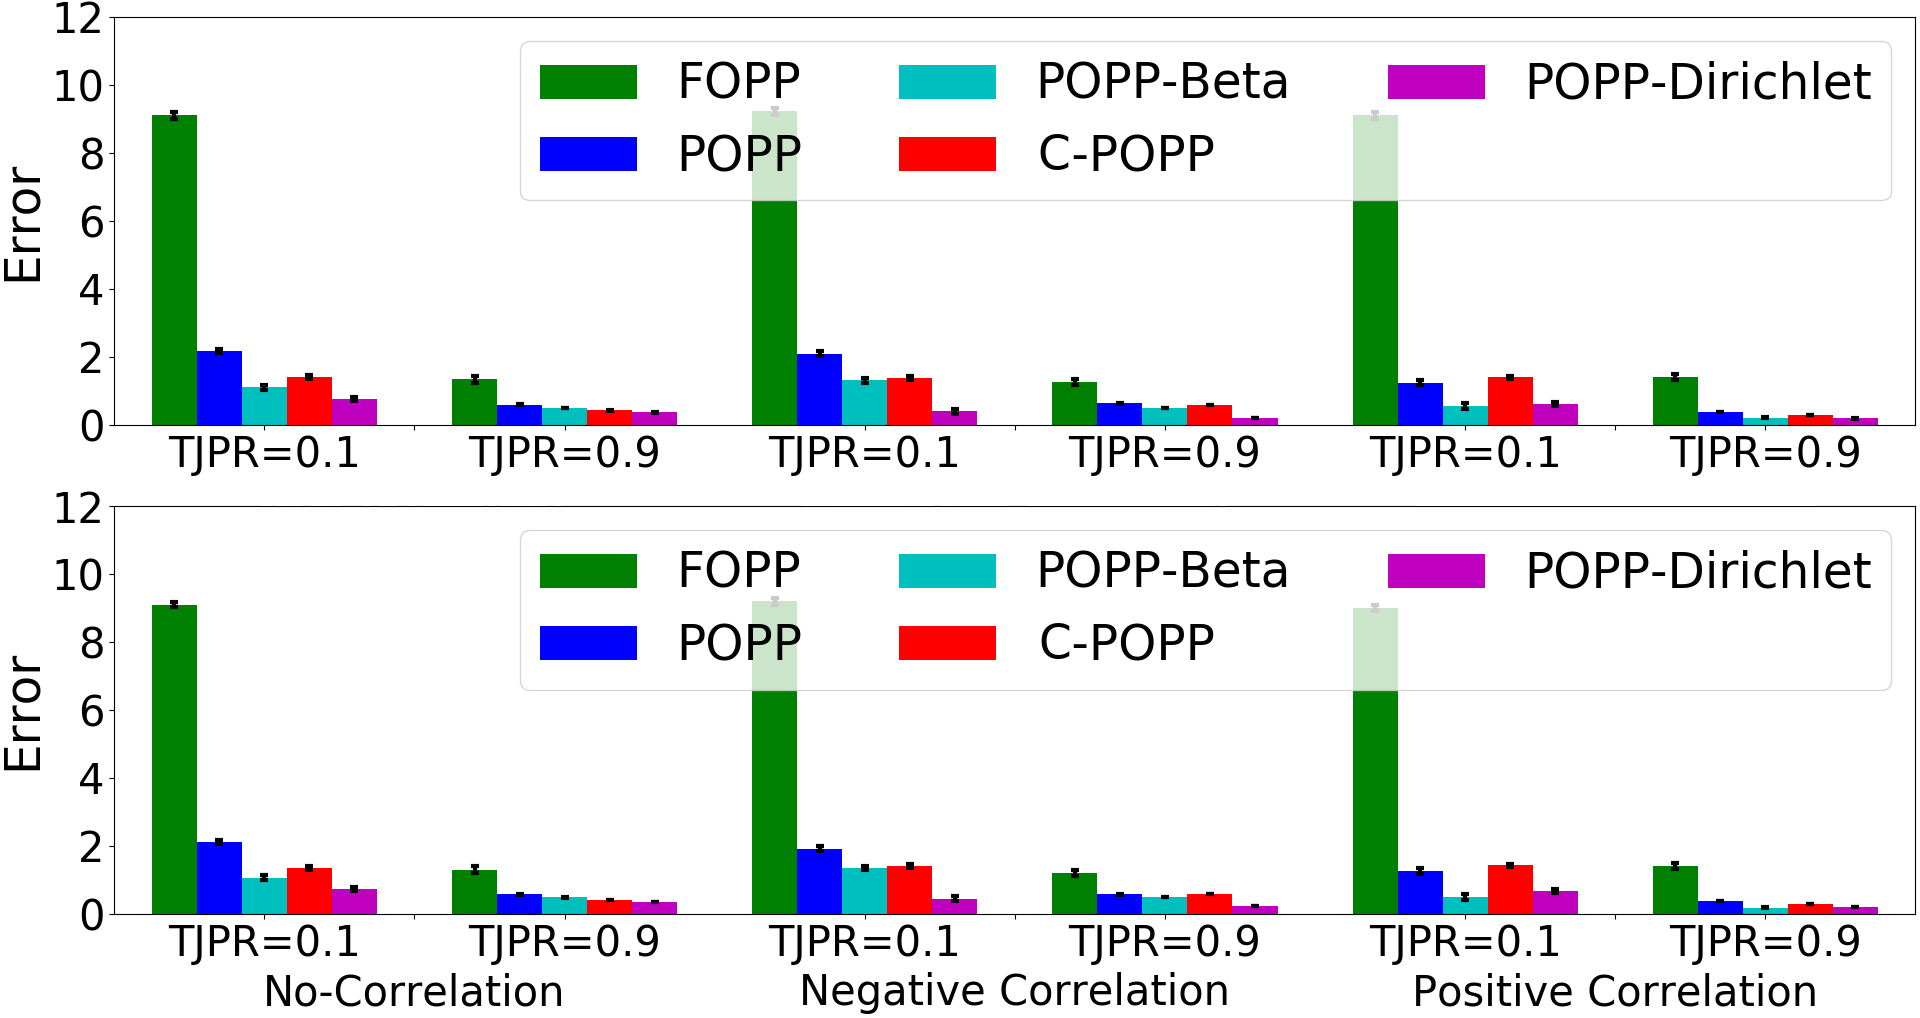
\includegraphics[width=0.8\textwidth]{./figures/tjpr_comparison_120.png}
    \caption{The RMSE of posterior estimates of $\lambda$ for the POPP and its variation models with 12 sample data used to build the (joint) sensor model with variation in $\mathcal{P^+}$. All models are compared to the FOPP model. Each trial consisted of a stream of $\protect\mathbf{s_1} \ldots \protect\mathbf{s_{144}}$ samples to update $P(\lambda \mid \protect\mathbf{s_i})$. Accuracies of MAP estimates are shown in the top panel, accuracies of expectation of the posterior in the bottom panel. Each data point is an average of 30 trials. Standard errors are shown.} 
	\label{fig:tjpr_comparison_120}
	\vspace{-20pt}
\end{figure}

\begin{figure}[t!]
	\centering
	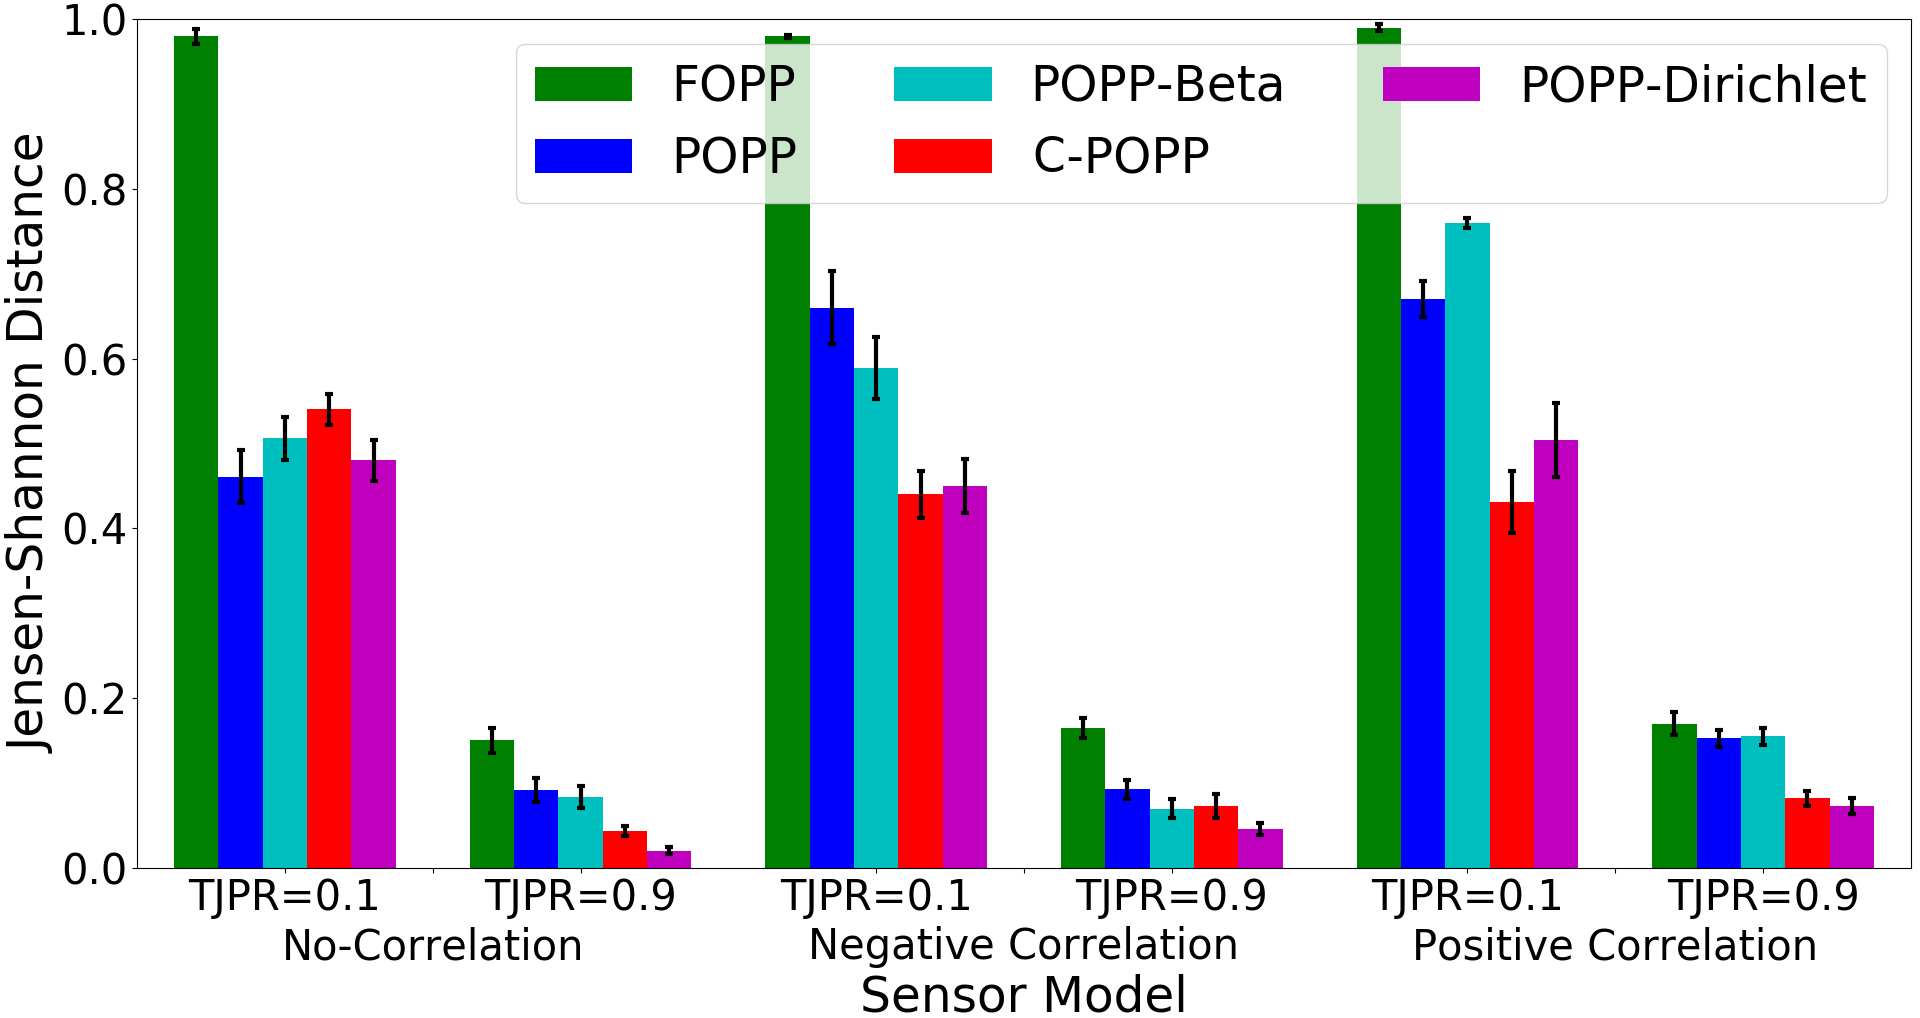
\includegraphics[width=0.8\textwidth]{./figures/tjpr_comparison_120_kl.png}
	\caption{The Jensen-Shannon distance of posterior estimates of $\lambda$ for the POPP and its variation models with 12 sample data used to build the (joint) sensor model with variation on $\mathcal{P^+}$. All models are compared to the FOPP model. Each trial consisted of a stream of $\protect\mathbf{s_1} \ldots \protect\mathbf{s_{144}}$ samples to update $P_G(\lambda \mid \protect\mathbf{s_i})$. Each data point is an average of 30 trials. Standard errors are shown.} 
	\label{fig:tjpr_comparison_120_kl}
	\vspace{-10pt}
\end{figure}

% Different correlations between two sensors were tested: positive correlation, negative correlation, and no correlation. These correlations are aimed to show the benefit of the C-POPP and POPP-Dirichlet models over the POPP and the POPP-Beta models. One should note that under the POPP and POPP-Beta models, sensors are assumed to be uncorrelated. For each correlation type, a further variation to different levels of sensor unreliability was considered. The true joint positive rate $\mathcal{E^+}$ (TJPR) and the true joint negative rate $\mathcal{E^-}$ (TJNR) were set as basis for varying sensor unreliability. For example, having TJPR configured with $P_{jnt}(d_{1k}=1, d_{2k}=1 ; e_k=1) = 0.1, P_{jnt}(d_{1k}=0, d_{2k}=0 ; e_k=1) = 0.9$ means that the true positive rate (TPR) for each sensor $j$ is $\textrm{\textit{tpr}}_j = P_j(d_k = 1; e_k=1) = 0.1$.

% First, two variations were made to the true joint positive rate $\mathcal{E^+}$ (TJPR), while fixing the true joint negative rate $\mathcal{E^-}$ (TJNR) on each type of correlation. This includes:
% \begin{itemize}
%     \item $P_{jnt}(d_{1k}=1, d_{2k}=1 ; e_k=1) = 0.1, P_{jnt}(d_{1k}=0, d_{2k}=0 ; e_k=1) = 0.9$ ($\mathcal{E^+}$ with low positive correlation);
%     \item $P_{jnt}(d_{1k}=1, d_{2k}=1 ; e_k=1) = 0.9, P_{jnt}(d_{1k}=0, d_{2k}=0 ; e_k=1) = 0.1$ ($\mathcal{E^+}$ with high positive correlation);
%     \item $P_{jnt}(d_{1k}=1, d_{2k}=0 ; e_k=1) = 0.05, P_{jnt}(d_{1k}=0, d_{2k}=1 ; e_k=1) = 0.05, P_{jnt}(d_{1k}=0, d_{2k}=0 ; e_k=1) = 0.9$ ($\mathcal{E^+}$ with low negative correlation);
%     \item $P_{jnt}(d_{1k}=1, d_{2k}=0 ; e_k=1) = 0.45, P_{jnt}(d_{1k}=0, d_{2k}=1 ; e_k=1) = 0.45, P_{jnt}(d_{1k}=0, d_{2k}=0 ; e_k=1) = 0.1$ ($\mathcal{E^+}$ with high negative correlation);
%     \item $P_{jnt}(d_{1k}=1, d_{2k}=0 ; e_k=1) = 0.033, P_{jnt}(d_{1k}=0, d_{2k}=1 ; e_k=1) = 0.033, P_{jnt}(d_{1k}=1, d_{2k}=1 ; e_k=1) = 0.033, P_{jnt}(d_{1k}=0, d_{2k}=0 ; e_k=1) = 0.901$ ($\mathcal{E^+}$ with no correlation -- Similar to a sensor model with TPR = 0.066);
%     \item $P_{jnt}(d_{1k}=1, d_{2k}=0 ; e_k=1) = 0.3, P_{jnt}(d_{1k}=0, d_{2k}=1 ; e_k=1) = 0.3, P_{jnt}(d_{1k}=1, d_{2k}=1 ; e_k=1) = 0.3, P_{jnt}(d_{1k}=0, d_{2k}=0 ; e_k=1) = 0.1$ ($\mathcal{E^+}$ with no correlation -- Similar to a sensor model with TPR = 0.6).
% \end{itemize}

% Second, two variations to the true joint negative rate $\mathcal{E^-}$ (TJNR), while fixing the true joint positive rate $\mathcal{E^+}$ (TJPR) on each type of correlation. This includes: 
% \begin{itemize}
% 	\item $P_{jnt}(d_{1k}=1, d_{2k}=1 ; e_k=0) = 0.1, P_{jnt}(d_{1k}=0, d_{2k}=0 ; e_k=0) = 0.9$ ($\mathcal{E^-}$ with low positive correlation);
% 	\item $P_{jnt}(d_{1k}=1, d_{2k}=1 ; e_k=0) = 0.9, P_{jnt}(d_{1k}=0, d_{2k}=0 ; e_k=0) = 0.1$ ($\mathcal{E^-}$ with high positive correlation);
% 	\item $P_{jnt}(d_{1k}=1, d_{2k}=0 ; e_k=0) = 0.05, P_{jnt}(d_{1k}=0, d_{2k}=1 ; e_k=0) = 0.05, P_{jnt}(d_{1k}=0, d_{2k}=0 ; e_k=0) = 0.9$ ($\mathcal{E^-}$ with low negative correlation);
% 	\item $P_{jnt}(d_{1k}=1, d_{2k}=0 ; e_k=0) = 0.45, P_{jnt}(d_{1k}=0, d_{2k}=1 ; e_k=0) = 0.45, P_{jnt}(d_{1k}=0, d_{2k}=0 ; e_k=0) = 0.1$ ($\mathcal{E^-}$ with high negative correlation);
% 	\item $P_{jnt}(d_{1k}=1, d_{2k}=0 ; e_k=0) = 0.033, P_{jnt}(d_{1k}=0, d_{2k}=1 ; e_k=0) = 0.033, P_{jnt}(d_{1k}=1, d_{2k}=1 ; e_k=0) = 0.033, P_{jnt}(d_{1k}=0, d_{2k}=0 ; e_k=1) = 0.901$ ($\mathcal{E^-}$ with no correlation -- Similar to a sensor model with low TNR);
% 	\item $P_{jnt}(d_{1k}=1, d_{2k}=0 ; e_k=0) = 0.3, P_{jnt}(d_{1k}=0, d_{2k}=1 ; e_k=0) = 0.3, P_{jnt}(d_{1k}=1, d_{2k}=1 ; e_k=0) = 0.3, P_{jnt}(d_{1k}=0, d_{2k}=0 ; e_k=1) = 0.1$ ($\mathcal{E^-}$ with no correlation -- Similar to a sensor model with moderate TNR).
% \end{itemize}

The performance of all POPP models was assessed by measuring how accurate each model is in estimating the true $\lambda'$. The true $\lambda'$ is estimated by applying the FOPP model on the true counts. Two options were used to measure the accuracy: (1) the RMSE of the expectation (mean) and the MAP hypothesis (mode) of each model posterior distribution over $\lambda$ to the true $\lambda'$; and (2)  the Jensen-Shannon distance between the posterior distribution $P(\lambda \mid \mathbf{s_i})$ and the distribution of the true $\lambda'$. 

\begin{figure}[t!]
	\centering
	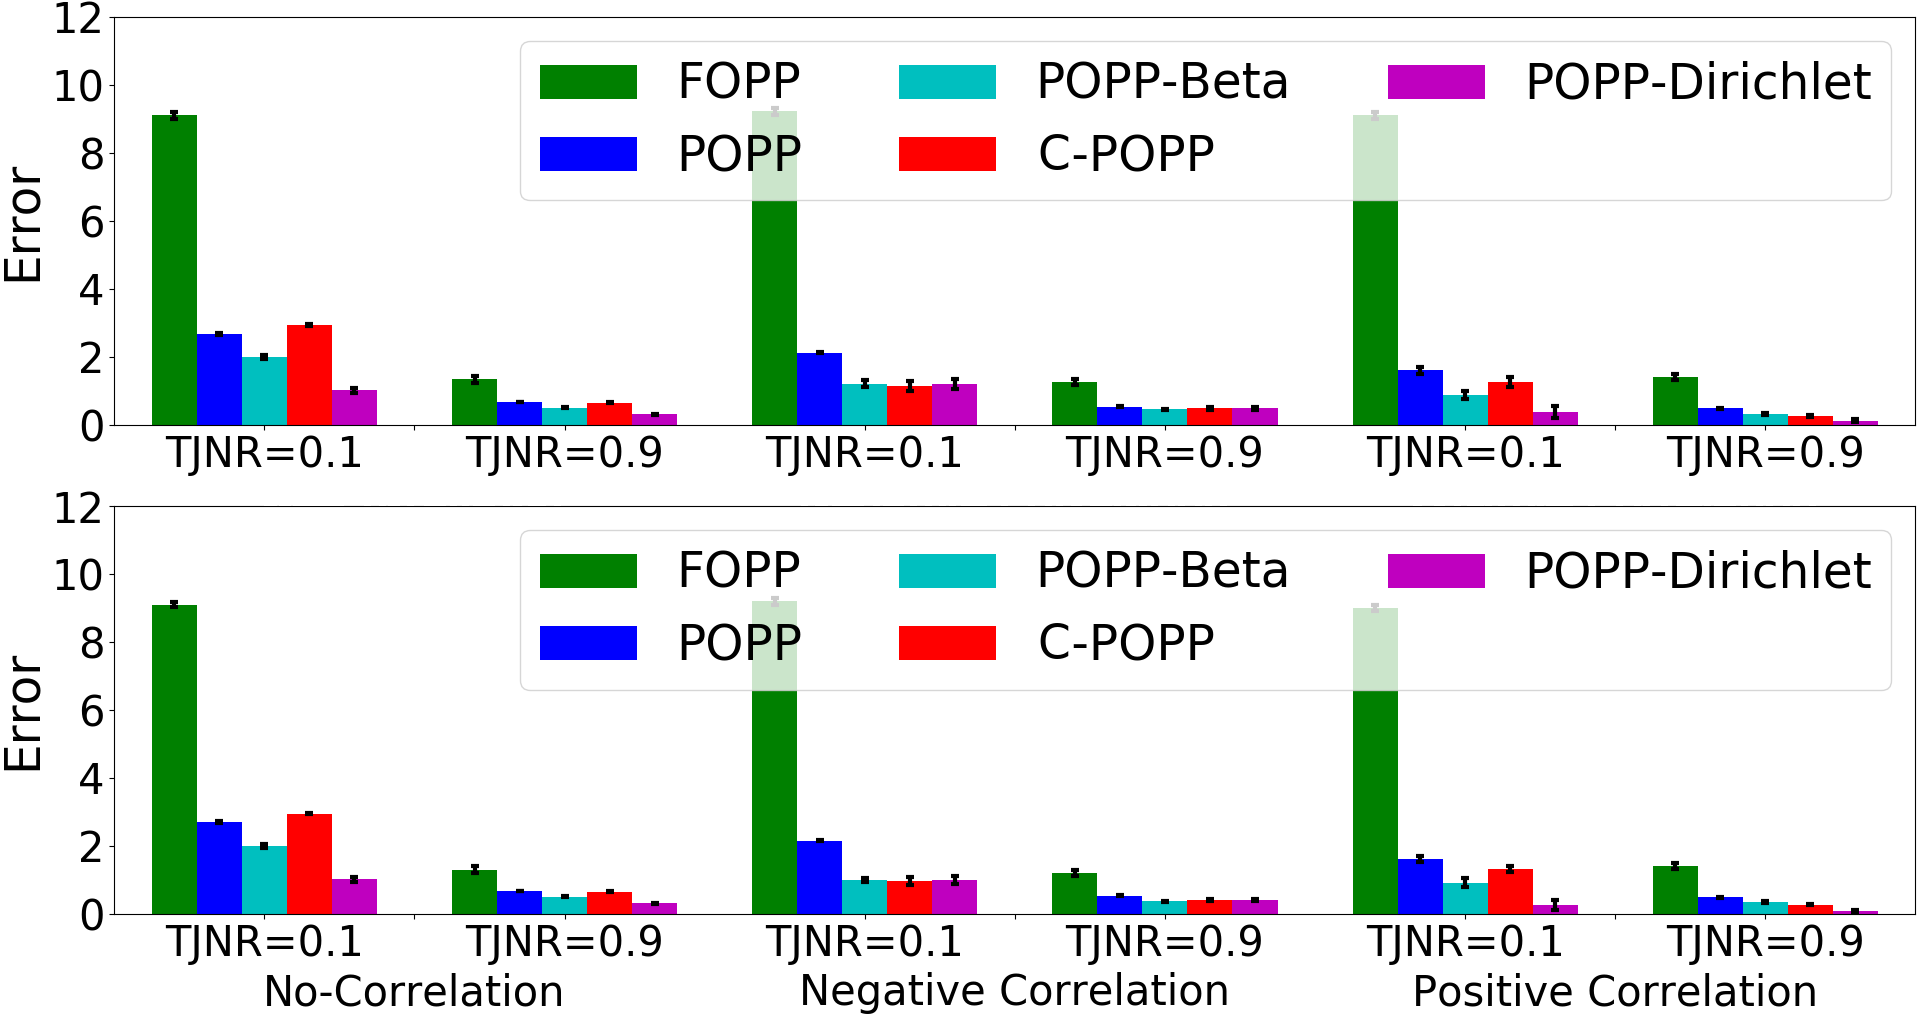
\includegraphics[width=0.8\textwidth]{./figures/tjnr_comparison_120.png}
    \caption{The RMSE of posterior estimates of $\lambda$ for the POPP and its variation models with 12 sample data used to build the (joint) sensor model with variation in $\mathcal{P^-}$. All models are compared to the FOPP model. Each trial consisted of a stream of $\protect\mathbf{s_1} \ldots \protect\mathbf{s_{144}}$ samples to update $P(\lambda \mid \protect\mathbf{s_i})$. Accuracies of MAP estimates are  in the top panel, accuracies of the expectation of the posterior in the bottom panel. Each data point is an average of 30 trials. Standard errors are shown.} 
	\label{fig:tjnr_comparison_120}
	\vspace{-20pt}
\end{figure}

\begin{figure}[t!]
	\centering
	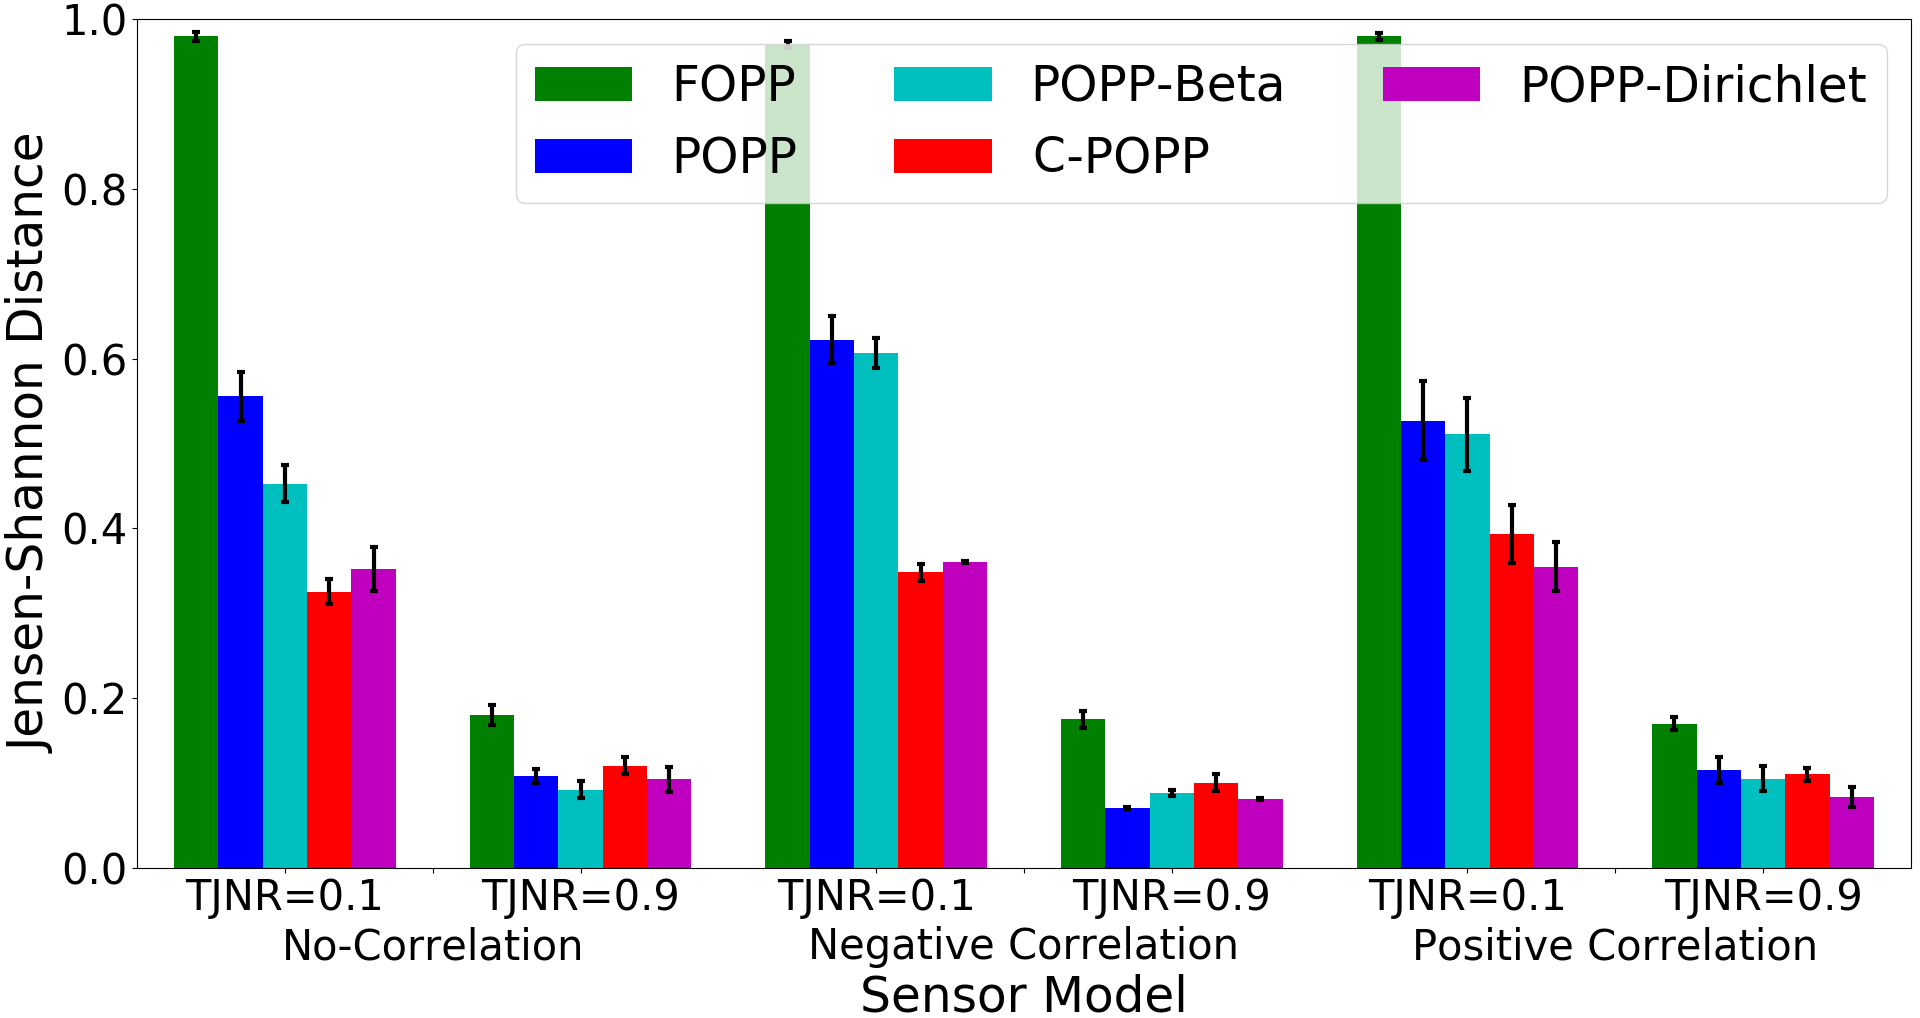
\includegraphics[width=0.8\textwidth]{./figures/tjnr_comparison_120_kl.png}
	\caption{The Jensen-Shannon distance of posterior estimates of $\lambda$ for the POPP and its variation models with 12 sample data used to build the (joint) sensor model with variation on $\mathcal{P^-}$. All models are compared to the FOPP model. Each trial consisted of a stream of $\protect\mathbf{s_1} \ldots \protect\mathbf{s_{144}}$ samples to update $P_G(\lambda \mid \protect\mathbf{s_i})$. Each data point is an average of 30 trials. Standard errors are shown.} 
	\label{fig:tjnr_comparison_120_kl}
	\vspace{-15pt}
\end{figure}

Figures \ref{fig:tjpr_comparison_120} and \ref{fig:tjpr_comparison_120_kl} show the accuracy of all POPP models over the variations of TJPR ($P^+$), whereas Figures \ref{fig:tjnr_comparison_120} and \ref{fig:tjnr_comparison_120_kl} show the accuracy across the variation in TJNR ($P^-$). From these figures, POPP-Beta and POPP-Dirichlet show a better accuracy than POPP and C-POPP. C-POPP and POPP-Dirichlet, which utilize correlations among sensors to estimate the arrival rate $\lambda'$, tend to be more accurate than the standard POPP and POPP-Beta.
In general, POPP-Dirichlet tends to be more accurate than any other POPP model thanks to its ability to model correlation among sensors \emph{and} how confident it is in its sensor model.
One should note that if the number of training samples for the (joint) sensor model is high, then the POPP-Dirichlet and the C-POPP should have similar posterior distributions. This is because the POPP-Dirichlet will have tight densities over the sensor models, and these should be comparable to the point estimates used in the C-POPP  sensor models.

In this paper, we remove computation time per sample analysis between POPP and its extensions because the computation relies heavily on the filters chosen. The time to calculate the distribution of sensed count given the actual count between POPP, POPP-Beta, C-POPP and the POPP-Dirichlet on each sample can be considered constant and, therefore, is negligible to the total computation time. Our prior work provided a detailed comparison in computational efficiency between different filters \cite{jovan18a}.

%!TEX root = ../sample.tex

\section{Evaluation on Aggregate Human Occupancy Behaviour Dataset}
\label{sec:evareal}

We now investigate the performance of the POPP model and its extensions on a real world dataset\footnote{The dataset can be downloaded from \url{https://github.com/ferdianjovan/spectral_popp}}.
% 
The dataset was gathered from an office building in which a mobile robot~\cite{hawes2016strands} counted the number of people in different regions whilst patrolling (see Figure~\ref{fig:map_popp_independent_test} for the map of the building). The dataset contains time series  counts from three different automated person detectors~\cite{dondrup2015real}. These use laser, depth camera and RGB information. We refer to these detectors respectively as the leg detector (LD), upper body detector (UBD), and change (or scenery) detector (CD). Each of these detectors acts as one sensor. Each returns a sensed count of the number of people it detected in each 10 minute interval during the day. To unify different frequency of detections of each sensor, we used the lowest frequency detection from the change detector and limited to maximum one detection per minute. These detectors are unreliable, as can be seen from Figure~\ref{fig:single_sensor_rate_transformation}, which shows examples of correct and incorrect detections.

\begin{figure}[t]
	\centering
	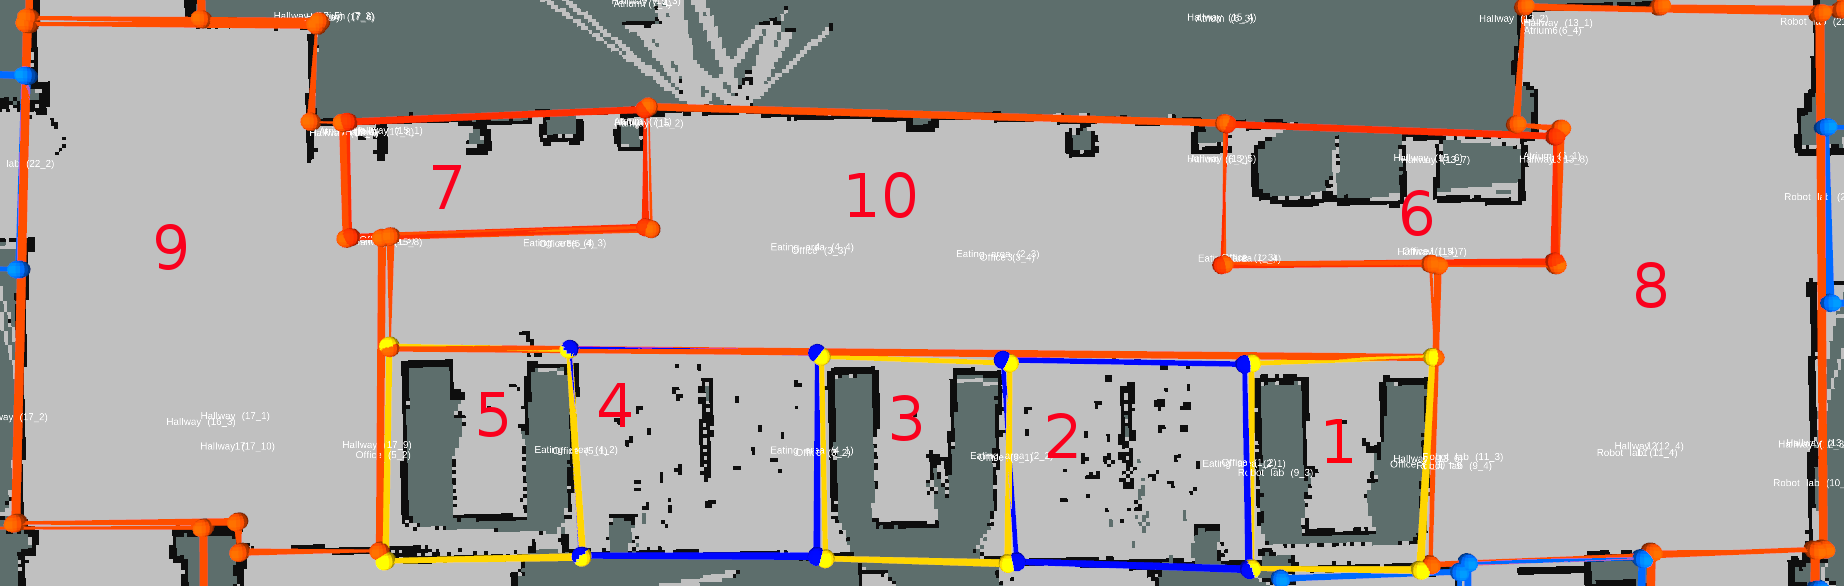
\includegraphics[width=0.8\columnwidth]{./figures/map_popp.png}
	\caption{The office building in which the robot gathered data. Areas are bounded by imaginary lines.}
	\label{fig:map_popp_independent_test}
	\vspace{-20pt}
\end{figure}

\begin{figure}[t]
	\centering
	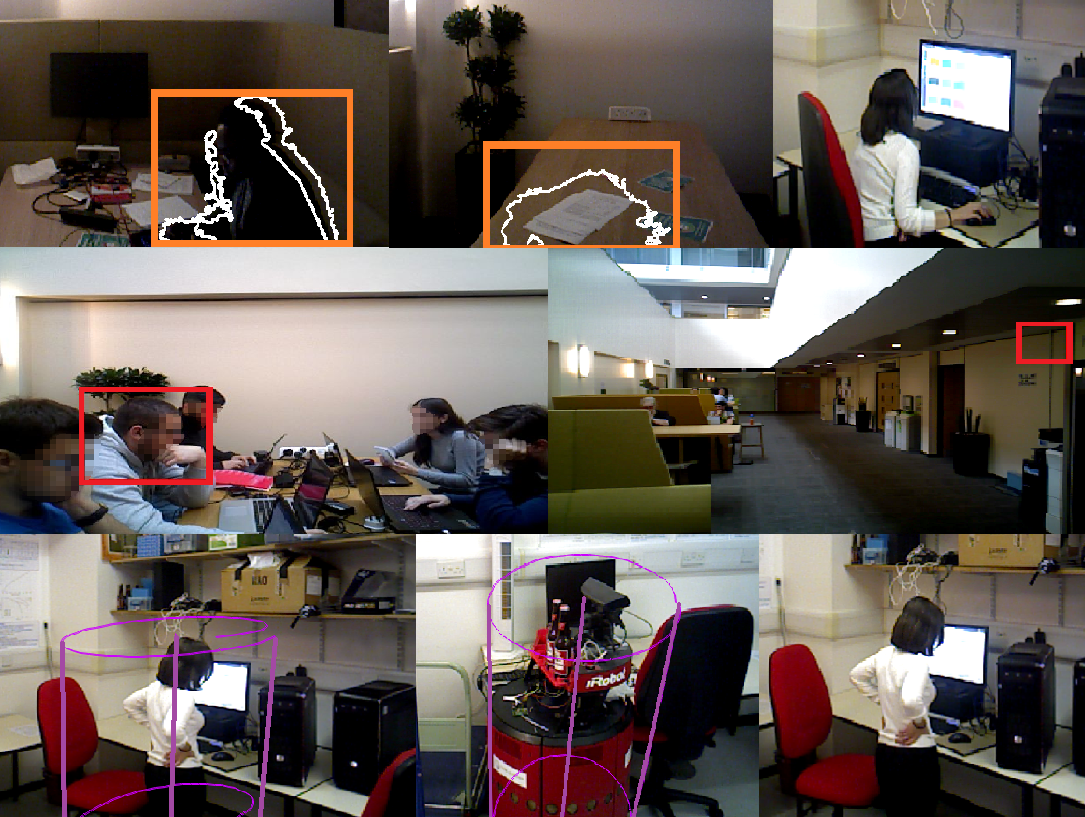
\includegraphics[width=0.8\columnwidth]{./figures/sensor_images.png}
	\caption{Correct and incorrect detections, and non-detections, from different regions in the environment for each sensor. Top row: change detector. Middle row: upper body detector. Bottom row: leg detector. Detections are marked with 2D or 3D bounding boxes. A bounding box containing a person is a correct detection (true positive). One without a person is an incorrect detection (false positive). A person without a bounding box is a missed detection (false negative).}
	\label{fig:single_sensor_rate_transformation}
	\vspace{-25pt}
\end{figure}

By comparing the ground truth with the detections made by sensors, we compute a sensor model for each region. An average of the sensor models across all regions can be seen in Table \ref{table:sensor_model_popp_beta}. Although the robot operated for 24 hours day, the sensor models were built using only the data collected from 10am to 8pm, since there were few detections outside these times. From a 69 day trial of the mobile robot, we obtained 48 days of usable observations. We specified a time interval for each Poisson distribution of 10 minutes, and recorded both the true counts and the detections made by each sensor in each interval. We assumed the underlying process in each region to be a periodic Poisson process in which there is a one-day periodicity, i.e. $\lambda(t) = \lambda(t + \Delta)$ with $\Delta = 24 * 60$ (minutes). This means that the expected number of people each day at a particular time is expected to be the same across the 48 days of observations. We estimated the true parameter $\lambda'(t)$ of the Poisson distribution at $t$ by running a FOPP model on the true counts within each interval. We use this estimate of $\lambda'(t)$ from the true counts as the target which the POPP models must estimate from the sensed counts.

The different POPP approaches rely on sensor models that must be calculated from a confusion matrix relating true counts to the sensed counts from the different sensors. To separate the training and testing data we performed four fold cross-validation with data splits being on whole days, i.e., we used 12 days of data as a training set for a sensor model and then used the remaining 36 days of data as a test set on which to test the inferences made by each model from the sensor counts.

\begin{table}[b]
	\centering
	\vspace{-20pt}
	\caption{Averaged sensor models across all areas trained from 48 days of data.}
	\label{table:sensor_model_popp_beta}
	\begin{tabular}{lccc}
		\noalign{\hrule height 1.1pt}\noalign{\smallskip}
		Sensor & True Positive & True Negative \\
		\noalign{\smallskip}\hline\noalign{\smallskip}
		Leg Detector & 0.387 & 0.951 \\
		Upper Body Detector & 0.356 & 0.882 \\
		Change Detector & 0.731 & 0.900 \\ 
		\noalign{\hrule height 1.1pt}\noalign{\smallskip}
	\end{tabular}
\end{table}

For the 36 days of test data, the different models each made predictions of the $\lambda(t)$ parameter of the Poisson. Given this, we recorded (1) the RMSE between the MAP hypothesis of each model posterior distribution over $\lambda(t)$ and the true $\lambda'(t)$ and (2) the Jensen-Shannon distance between the posterior distribution $P(\lambda(t) \mid \mathbf{s_i})$ and the distribution of the true $\lambda'(t)$. Using these metrics, we compared the performance of all POPP models (estimated using the switching filter described in~\ref{sec:estimators}) to the Bayes' filter arising from the FOPP model. The FOPP model is a single sensor model and was estimated from the change detector counts since this was the most reliable detector among the three available (as shown in Table~\ref{table:sensor_model_popp_beta}). 

Figures \ref{fig:fopp_popp_popb_npop_popd_rmse_evo} and \ref{fig:fopp_popp_popb_npop_popd_kl_evo} show the accuracy comparison between all POPP models and the standard FOPP model over time. It can be seen that all models become more accurate as the days pass. All POPP models show more accuracy over the standard FOPP model. The $\lambda(t)$ estimate produced by the POPP-Dirichlet model is more accurate than the ones produced by the standard POPP model and the POPP-Beta model. However, the POPP-Dirichlet estimate is not always more accurate than the one produced by the C-POPP model. 

As the POPP-Dirichlet model is more conservative in estimating the parameter $\lambda(t)$ than the C-POPP model, the estimate moves more slowly towards the true $\lambda'(t)$. This is seen in Figure~\ref{fig:fopp_popp_popb_npop_popd_kl_evo}.
By the third day, the POPP-Dirichlet model outperformed the POPP, POPP-Beta, and C-POPP models in terms of accuracy. However, the accuracy gap between the C-POPP model and the POPP-Dirichlet model becomes smaller over time. By the 36th day the C-POPP model outperforms the POPP-Dirichlet by a small margin. It should be noted that Figures \ref{fig:fopp_popp_popb_npop_popd_rmse_evo} and \ref{fig:fopp_popp_popb_npop_popd_kl_evo} are averaged RMSE and the Jensen-Shannon distance from 10 different regions over time. The more regions with high volume of data available, the more accurate the joint sensor model, especially for C-POPP, will be and, in turns, the more accurate the C-POPP filter becomes in estimating the parameter $\lambda(t)$.

\begin{figure}[t!]
	\centering
	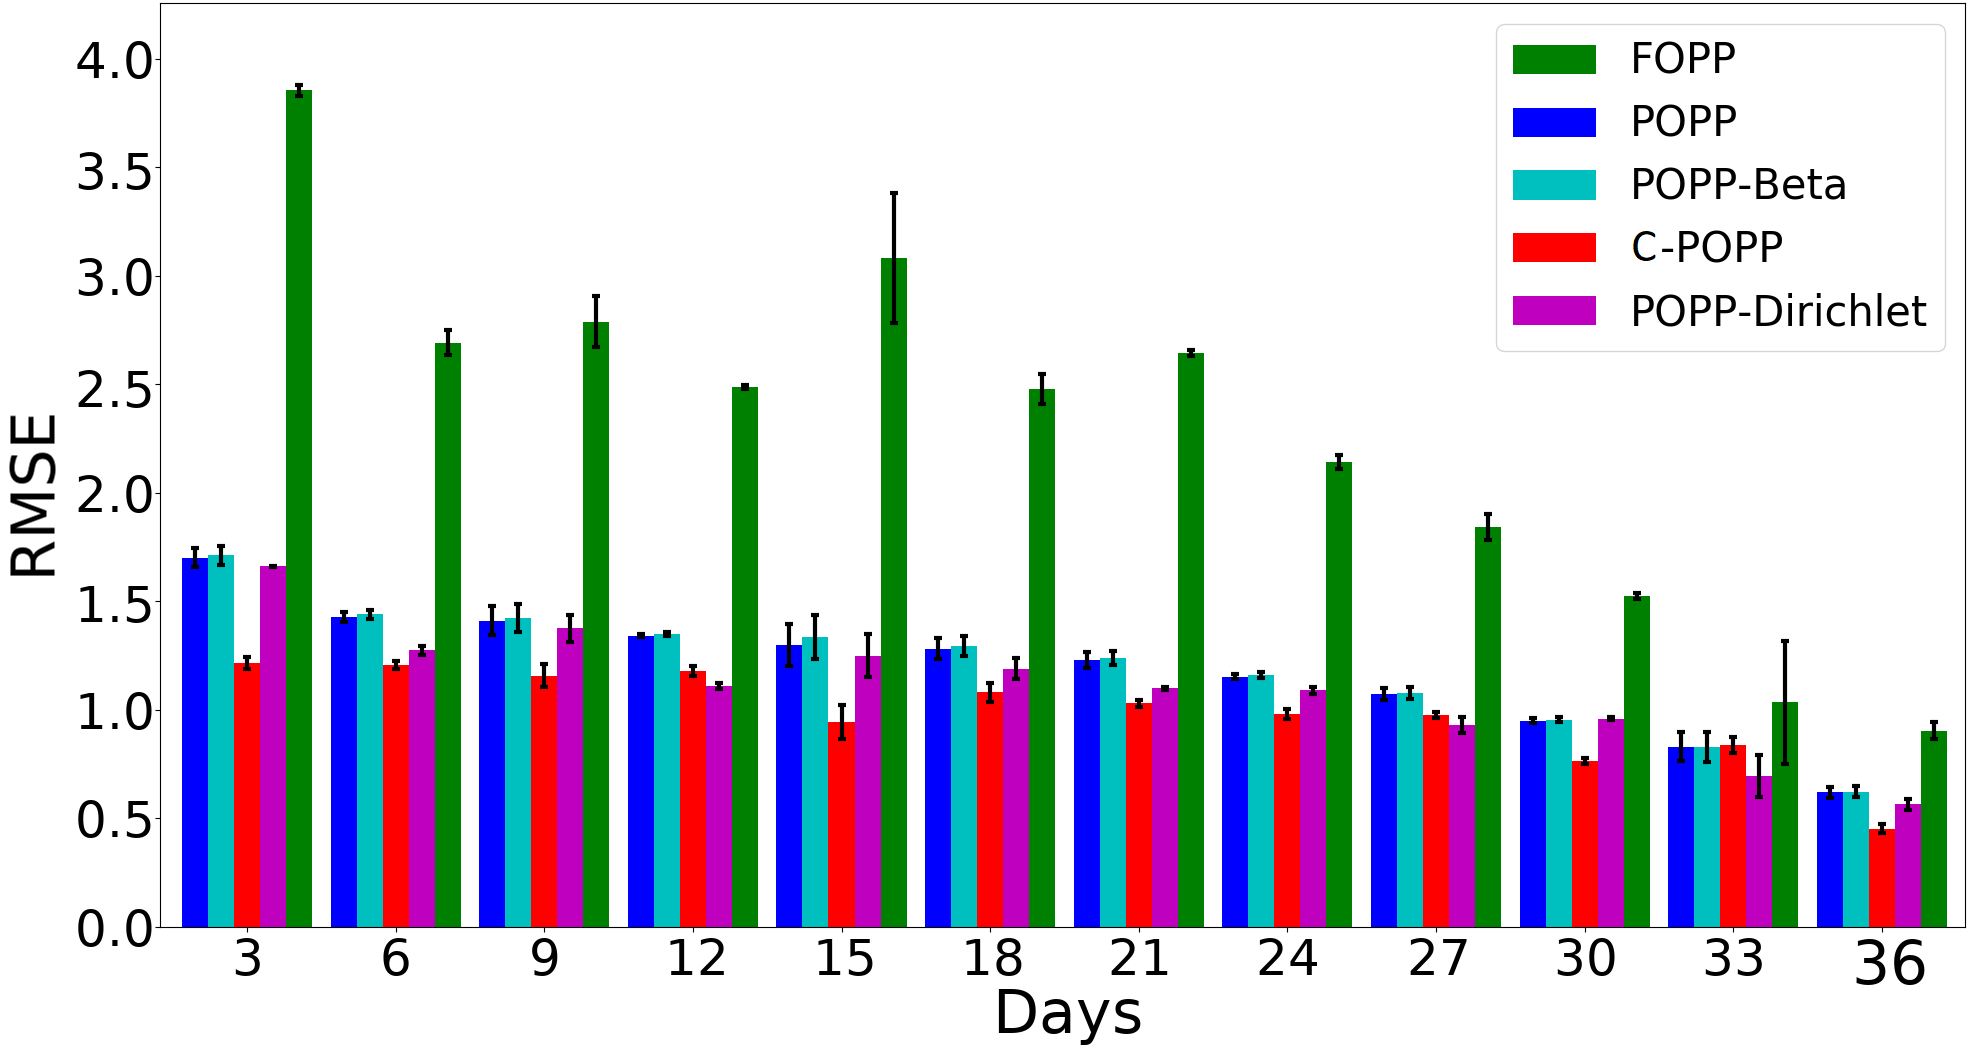
\includegraphics[width=0.8\columnwidth]{./figures/fopp_popp_popb_npop_popd_rmse_evo.png}
	\caption{The RMSE evolution of periodic Poisson processes with POPP, POPP-Beta, C-POPP, POPP-Dirichlet and FOPP filters from day 3 to day 36, averaged across all regions. Standard error is shown.}
	\label{fig:fopp_popp_popb_npop_popd_rmse_evo}
	\vspace{-10pt}
\end{figure}

\begin{figure}[t!]
	\centering
	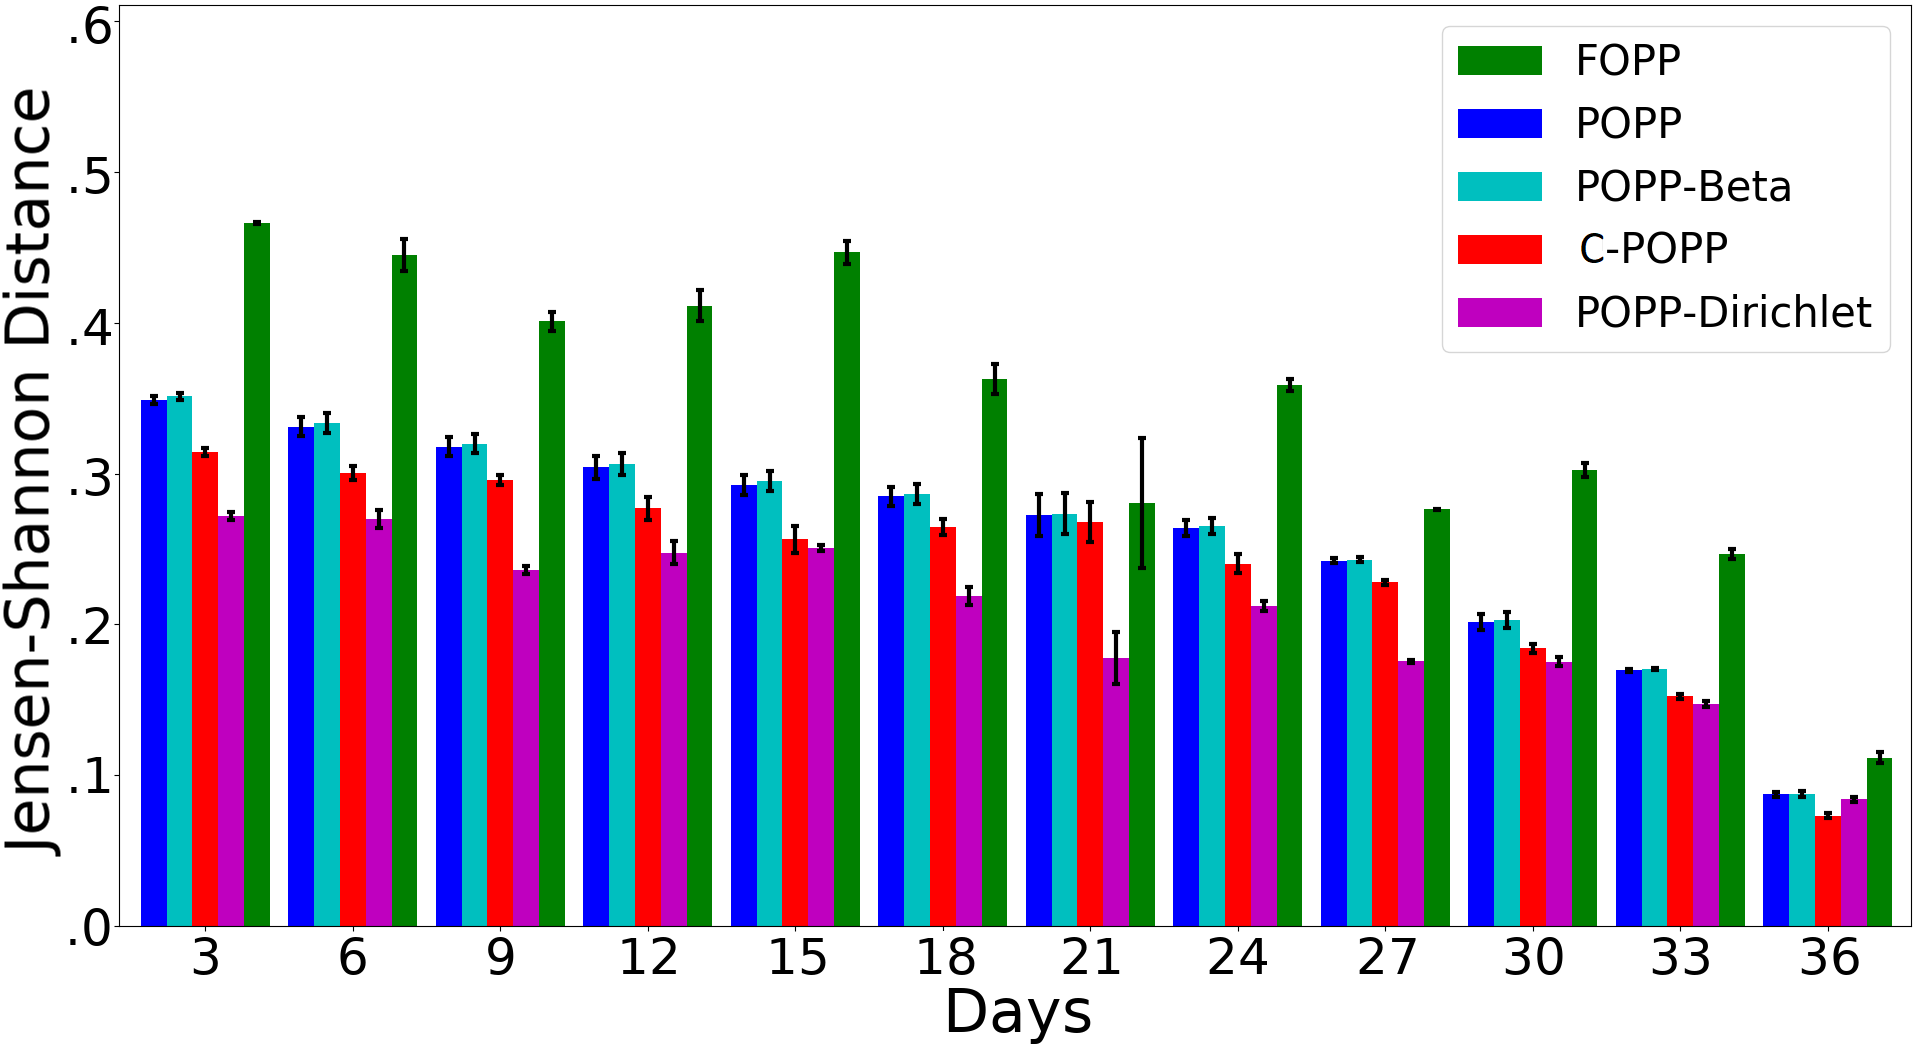
\includegraphics[width=0.8\columnwidth]{./figures/fopp_popp_popb_npop_popd_kl_evo.png}
	\caption{The Jensen-Shannon distance evolution of the FOPP, the POPP, the POPP-Beta, the C-POPP, and the POPP-Dirichlet filters in periodic Poisson processes from day 3 to day 36 in a 3-day interval, averaged across all regions. Standard error is shown.}
	\label{fig:fopp_popp_popb_npop_popd_kl_evo}
	\vspace{-25pt}
\end{figure}

\begin{figure}[t!]
	\centering
	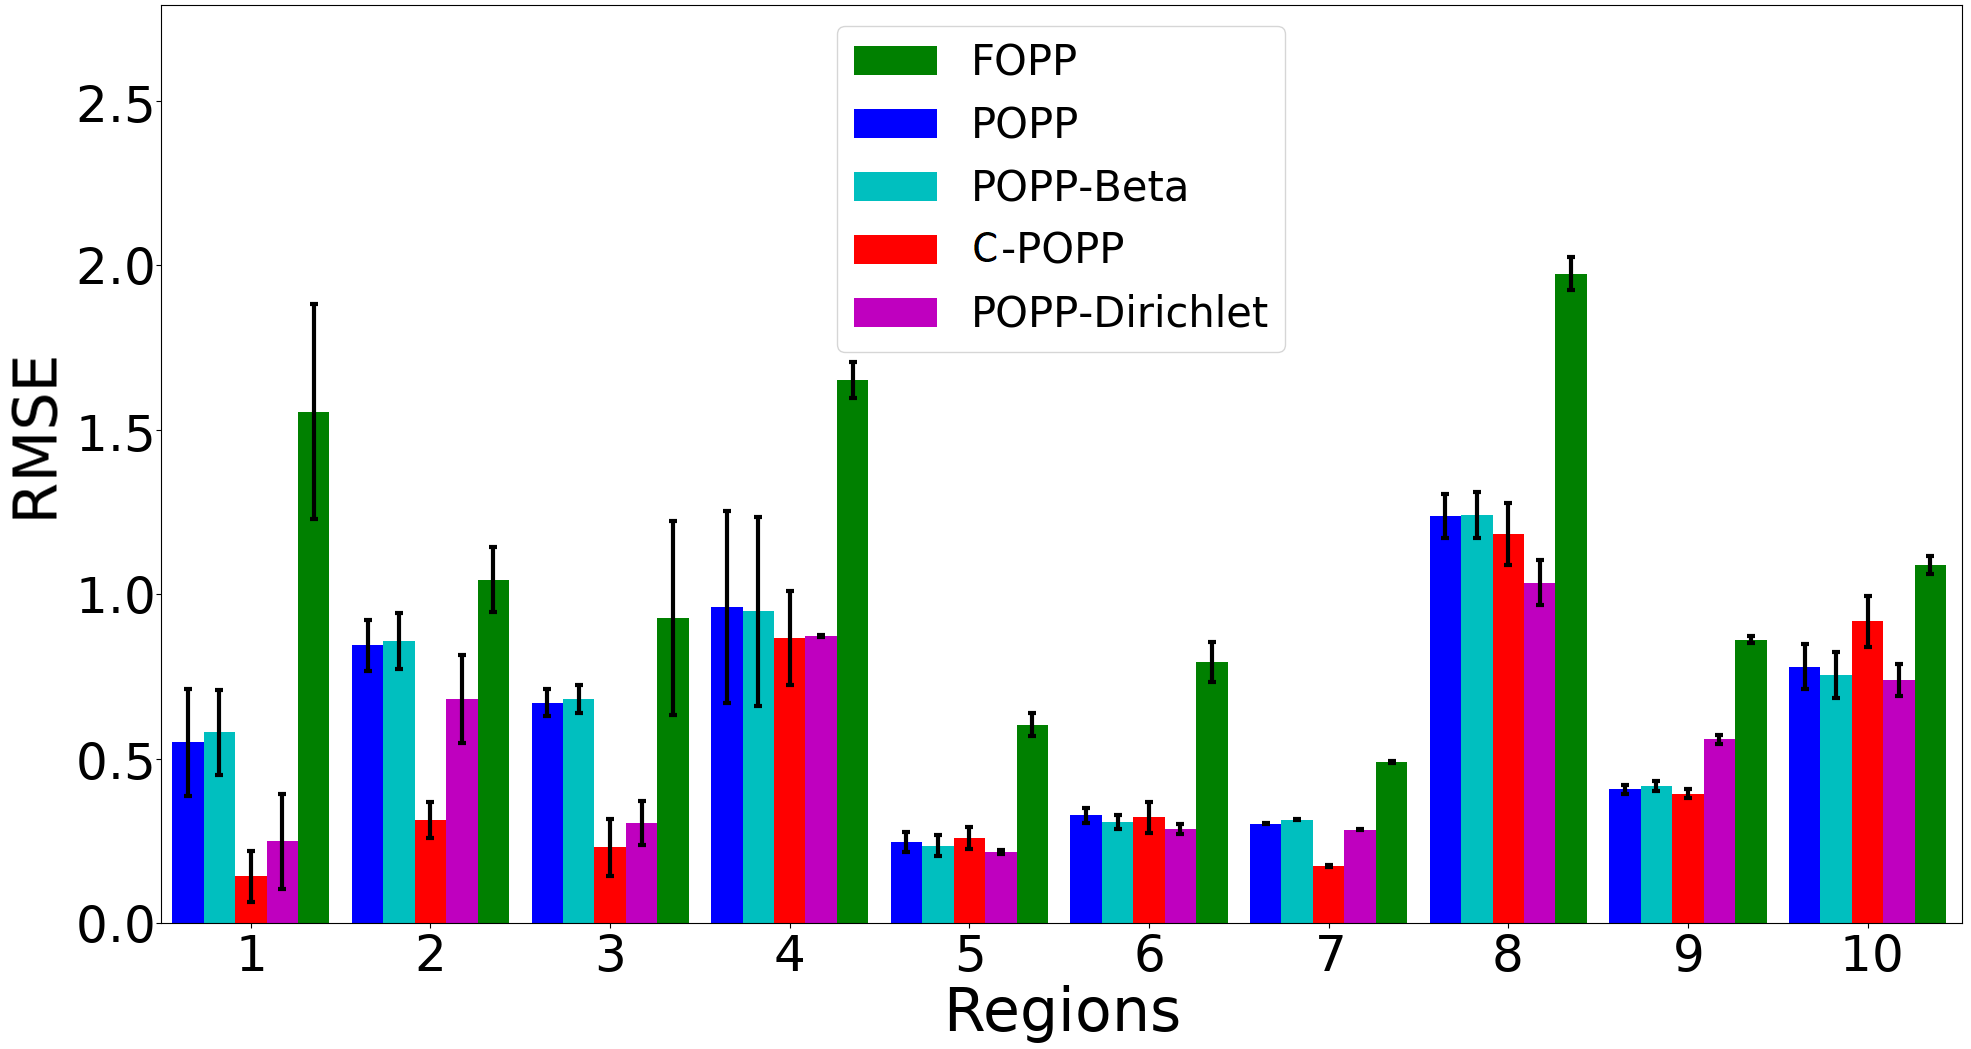
\includegraphics[width=0.8\columnwidth]{./figures/fopp_popp_popb_npop_popd_rmse.png}
	\caption{The RMSE of the FOPP, POPP, POPP-Beta, C-POPP, and POPP-Dirichlet filters across regions. The RMSE(s) are taken at the 36th day. Standard error is shown.}
	\label{fig:fopp_popp_popb_npop_popd_rmse}
	\vspace{-10pt}
\end{figure}

\begin{figure}[t!]
	\centering
	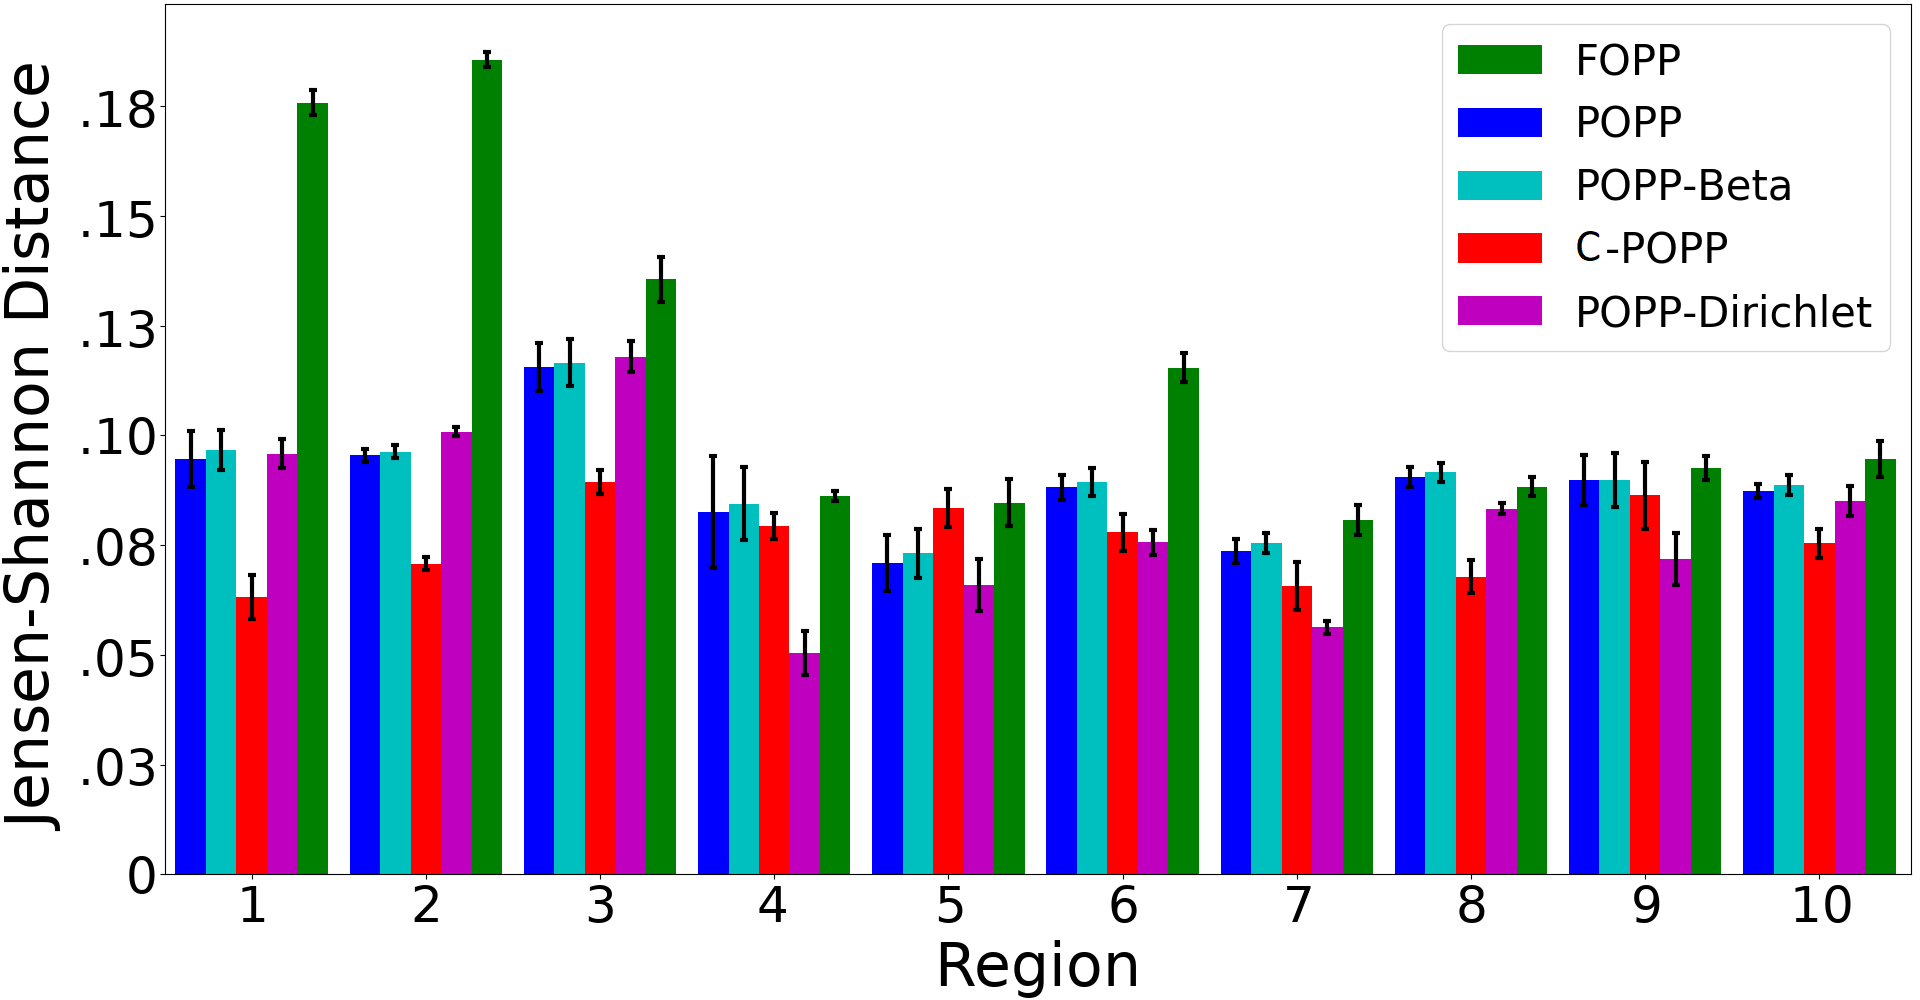
\includegraphics[width=0.8\columnwidth]{./figures/fopp_popp_popb_npop_popd_kl.png}
	\caption{The Jensen-Shannon of the FOPP, POPP, POPP-Beta, C-POPP, and POPP-Dirichlet filters across regions. The Jensen-Shannon value(s) are taken at the 36th day. Standard error is shown.}
	\label{fig:fopp_popp_popb_npop_popd_kl}
	\vspace{-20pt}
\end{figure}

Figure \ref{fig:fopp_popp_popb_npop_popd_rmse} and \ref{fig:fopp_popp_popb_npop_popd_kl} show the RMSE and Jensen-Shannon comparison between all POPP models and the FOPP across different regions by the end of the 36th day. It can be seen that the POPP-Dirichlet and the C-POPP once again outperformed the other models. Some regions such as 1, 2, and 3 have much more data than other regions. Since this  provides  more data to create the sensor models than other regions, the point-estimate joint sensor model for the C-POPP filter can be more accurately estimated for these regions. Unlike C-POPP filter, the POPP-Dirichlet estimates the joint sensor model as a distribution. This drives the POPP-Dirichlet slower and more conservative in estimating the parameter $\lambda(t)$ than the C-POPP model. Together with the choice of Dirichlet prior that follows uniform distribution, the POPP-Dirichlet requires more data to accurately estimate its joint sensor model.

The POPP-Dirichlet has an advantage on regions with low volume of data such as region 4, 5, 6 and 7. As some of these data were used to construct the joint sensor model for both C-POPP and the POPP-Dirichlet, a small amount of data creates an inaccurate point-estimate joint sensor model, which is used by the C-POPP filter. These problem is handled appropriately on the POPP-Dirichlet with its distribution joint sensor model with the help of Dirichlet prior as explained in Section \ref{subsec:popd}.

One interesting finding here is that there is small to no difference in performance between the POPP and the POPP-Beta filters on region 4, 5, 6, and 7. One would have thought that the performance of these two filters should follow the C-POPP and the POPP-Dirichlet filters. We argue that the volume of data used to create the sensor models for both POPP and the POPP-Beta were enough for an accurate estimate of point-estimate sensor model (POPP) and distribution sensor model (POPP-Beta). However, due to high correlations among sensors which were not captured by both the POPP and the POPP-Beta sensor models, the accuracy in estimating the parameter $\lambda(t)$ is worse than the C-POPP and the POPP-Dirichlet. It is also worse for the POPP-Beta filter since the POPP-Beta is more conservative in estimating the parameter $\lambda(t)$ than the POPP model. For example, region 4 contains high tables and tall chairs where the leg detector tended to falsely detected them as a person. Unless an upper body detector detects a person, the leg detector detection may be ignored. On the other hand, region 7 is a hallway with a water dispenser around the corner. This water dispenser is often falsely detected as a person by the upper body detector and the leg detector detections helps in reducing this mistake.

% One should remember there are only six hyperparameters needed estimate for the sensor model in the POPP and the POPP-Beta compared to sixteen hyperparameters needed estimate for the joint sensor model in the C-POPP and the POPP-Dirichlet. 

%Similar to the C-POPP model, the POPP-Dirichlet model is able to cope and overcome the problems with limited sample data both for building the joint sensor model and estimating the $\lambda(t_i, t_j)$. In many regions, the POPP-Dirichlet managed to show better estimates as well as more similar distributions than the POPP, the POPP-Beta, and the FOPP models. However, the POPP-Dirichlet filter falls behind both in accuracy (RMSE) and distribution similarity compared to the C-POPP model. This is attributed to the POPP-Dirichlet conservative way in estimating the parameter $\lambda(t_i, t_j)$ compared to the C-POPP model.
%!TEX root = ../bare_jrnl.tex

\section{Exploring for Human Activities}
\label{sec:exploration}

So far, the paper has focused on Bayesian methods for inferring a belief state about the spatio-temporal patterns of human occupancy from unreliable sensors. Given such a belief state a robot may plan how to actively explore to acquire new information so as to complete a task~\cite{hanheide2017robot, sridharan2019reba}. Here, the robot uses predicted counts from the belief state to \emph{explore} so as to detect human activities with increasing efficiency. 

Specifically, the robot's choice is whether to explore new region-time combinations or to exploit region-time combinations that are known to yield a high number of activities. This an instance of an \emph{exploration-exploitation} problem. Exploration-exploitation problems arise whenever an agent lacks an adequate model of the process it must control. At each moment, the agent chooses either to explore so as to improve the model or to exploit the existing model so as to maximise immediate performance. 
% In each time the robot has a choice between many actions, each of which both explores and exploits a certain place, but to varying degrees. As its goal is to maximise the reward gathered–as in getting as much data on human activities (by seeing as many humans) as possible–given its limited operational life, it is preferable to have a policy that is as near optimal as possible.

While exploration-exploitation problems in reinforcement learning, are typically intractable, there are well known, fast to compute, approximations~\cite{wyatt1998exploration, 1413255, AUDIBERT20091876}. One such approach is to use the upper bound of a probability distribution over the quantity being maximised. This causes the decision-making agent to exploit high-scoring, certain estimates, and explore highly uncertain estimates. In our robot exploration, for example, when the robot visits a place, it can be because the place either actually has high number of people (\textit{exploitation}) or potentially has high number of people (\textit{exploration}). In our case we use an upper bound on the arrival rate ($\lambda$) of a Poisson process ($\lambda_{UB}$) to choose the region for the robot to visit next. The upper bound of the probability interval of the arrival rate of a Poisson process is calculated as follows:

\begin{equation}
	\label{eq:upper_bound_exploration}
	\begin{tabular}{r@{ = }l}
	$\lambda_{UB}(t_i, t_j)$ & $\displaystyle \int_{t_i}^{t_j} CDF^{-1}(\% = 0.95 \mid \alpha_t, \beta_t)~dt$\\ [1ex]
	\end{tabular}
\end{equation}

\noindent with $\lambda_{UB}(t_i, t_j)$ as the upper bound of $\lambda$ within time $t_i$ and $t_j$, $i, j \in \{1, \ldots, \Delta\}$, and $CDF^{-1}$ as the inverse of the cumulative density function of a Gamma distribution. Given the upper bounds $\lambda^{r}_{UB}(t_i, t_j)$ for each region $r$ from the set of all regions $R$, the region to be visited between time $t_i$ and $t_j$ is chosen by:

\begin{equation}
\label{eq:choosing_place}
\underset{r \in \mathcal R}{\arg\max}~\lambda^{r}_{UB}(t_i, t_j)
\end{equation}
\noindent Figure~\ref{fig:map_vs_ub} depicts a comparison between the MAP hypothesis estimate and the upper bound estimate of a Poisson process.

\begin{figure}[t!]
	\centering
	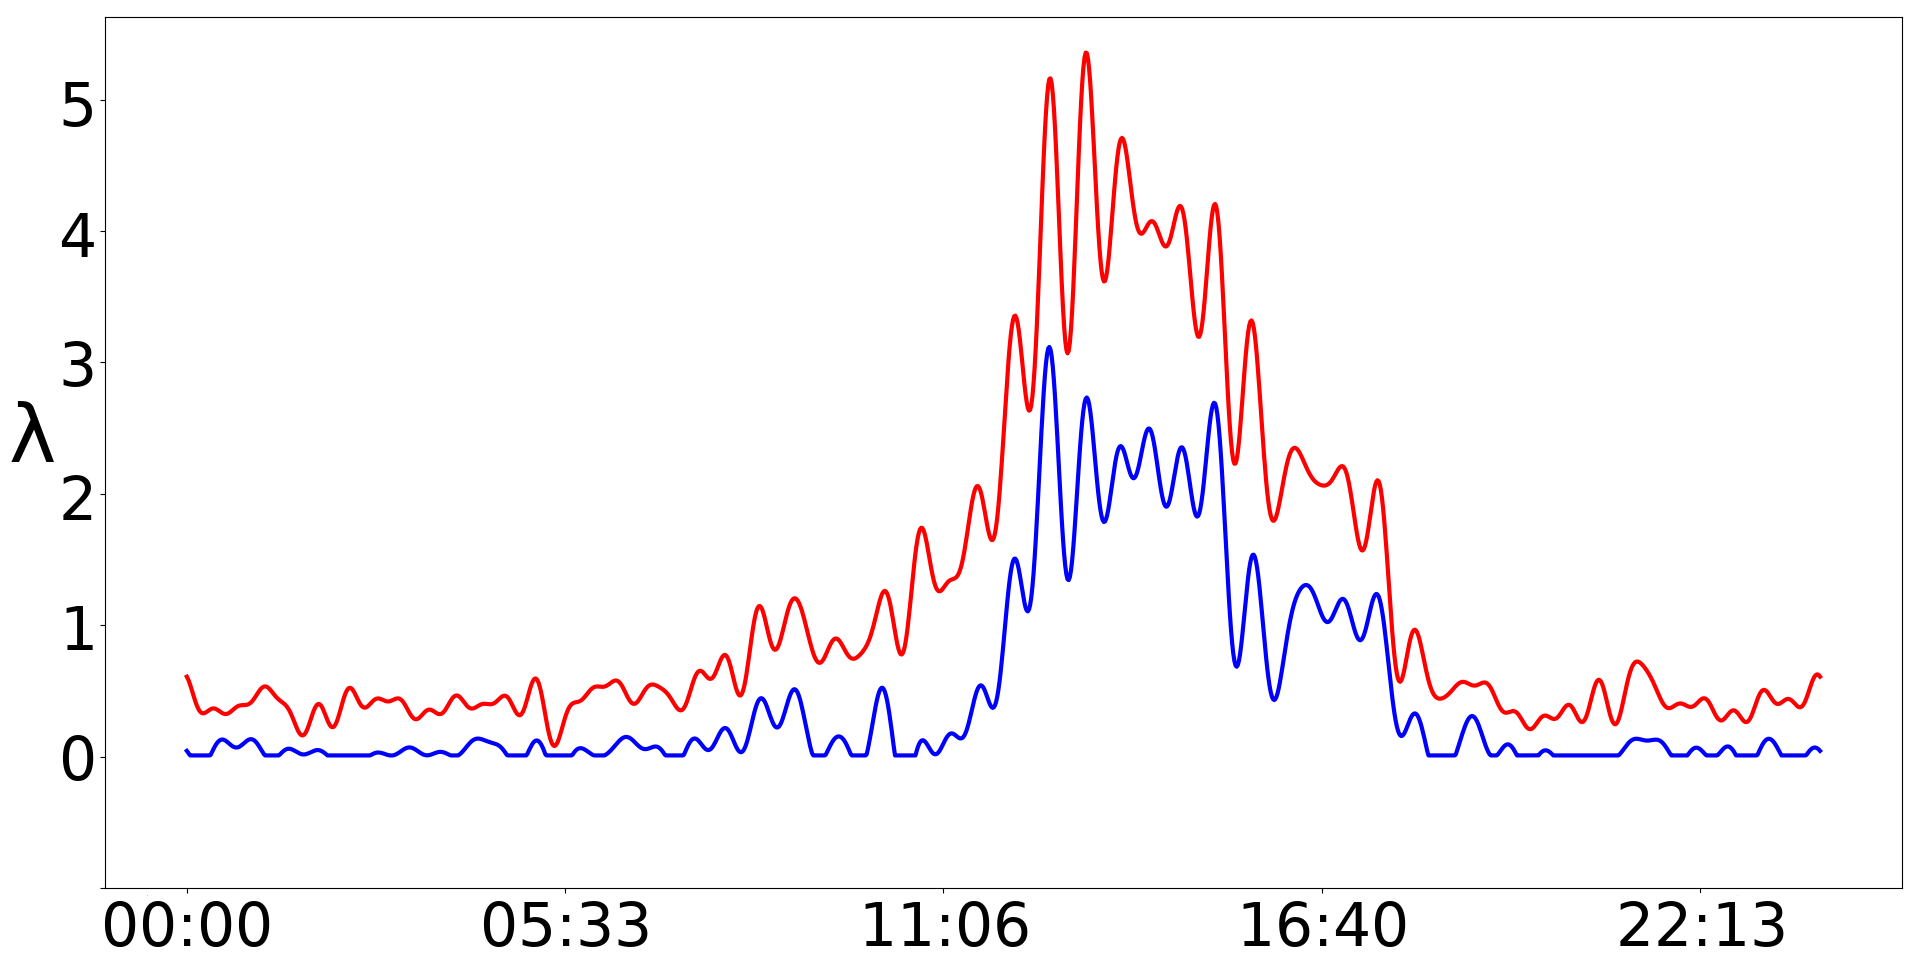
\includegraphics[width=0.5\textwidth]{./figures/map_vs_ub.png}
	\caption{A spectral Poisson process of region 9 (see Figure \ref{fig:map_popp_independent_test}) represented by its MAP hypothesis (blue line) and its upper bound of the probability interval (red line).}
	\label{fig:map_vs_ub}
\end{figure}


To tie the estimate of a particular Poisson process over a time interval to data collected previously, as in Section~\ref{sec:evareal} we assume that human presence in each region follows a \emph{periodic} Poisson process with daily periodicity. This allows us to regularise, and fill missing data, across the point estimates of upper bounds using methods based on the Fourier transform.  This exploits assumptions and algorithms introduced in our prior work. In particular, the series of upper bounds $\lambda_{UB}(t_i, t_j)$ are encoded and extracted via spectral analysis with the $l$-AAM technique described in~\cite{jovan_iros16}. The plot in Fig.~\ref{fig:map_vs_ub} shows how a spectral Poisson process look like, i.e., the effects of the spectral processing on a periodic Poisson process. Algorithm 2 depicts the process of computing the upper bound of a Poisson process and applying spectral analysis to it. We use this approach with upper bounds produced by our previously presented estimators: FOPP, POPP, and POPP-Beta. C-POPP and POPP-Dirichlet estimators are excluded in our experiments due to a need to limit experimental time to ~45 days to keep building use conditions that were broadly the same.\footnote{The experiments were conducted during a single academic semester within a university building.}

\begin{figure}[t!]
	\begin{center}
		\begin{tabular*}{0.5\textwidth}{l @{\extracolsep{\fill}}}
			\hline
			\textbf{l-AAM} \textrm{\cite{jovan_iros16}} \\
			\hline
			\textbf{Input:} $x_1, \ldots, x_n$: input signal, \\
			\hspace{0.3cm} total: maximum total frequency \\
			\textbf{Output:} $\mathcal S$: a collection of $(s, p, f)$ \\
			\textbf{Procedure:}\\
			\hspace{0.3cm} 1. Init. k $\leftarrow$ 0 \\
			\hspace{0.3cm} // Get frequency $0$ with Discrete Fourier Transform \\
			\hspace{0.3cm} 2. $[s, p, f] \leftarrow DFT(x_1, \ldots, x_n)[0]$\\
			\hspace{0.3cm} 3. $\mathcal S[k] \leftarrow [s, p, f]$ \\
			\hspace{0.3cm} 4. Repeat until k $>$ total \\
			\hspace{0.7cm} $\bullet ~ k \leftarrow k + 1$ \\
			\hspace{0.7cm} // Get the frequency with the highest amplitude \\
			\hspace{0.7cm} $\bullet ~ [s, p, f] \leftarrow \argmax_s DFT(x_1, \ldots, x_n)$ \\
			\hspace{0.7cm} // Update $\mathcal S$ with frequency $f$ \\
			\hspace{0.7cm} $\bullet$ if $f \in \mathcal S$, $[s', p', f'] \leftarrow \mathcal S[k', f'=f]$ \\
			\hspace{2.5cm} $s \leftarrow s + s'$; $p \leftarrow p + p'$ \\ 
			\hspace{0.7cm} $\bullet$ $\mathcal S[k] \leftarrow [s, p, f]$ \\
			\hspace{0.7cm} // Create a cosine signal from $f$ \\
			\hspace{0.7cm} $\bullet ~ x'_1, \ldots, x'_n \leftarrow s * ~ cos(2 \pi * f + p)$ \\
			\hspace{0.7cm} // Subtract current $x_1, \ldots, x_n$ with the cosine signal \\
			\hspace{0.7cm} $\bullet ~ x_1, \ldots, x_n \leftarrow x_1, \ldots, x_n - x'_1, \ldots, x'_n$ \\
			\hline
		\end{tabular*}	
	\end{center}
\end{figure}

\begin{figure}[t!]
	\begin{center}
		\begin{tabular*}{0.5\textwidth}{l @{\extracolsep{\fill}}}
			\hline
			\textbf{Algorithm 2} \textit{Upper Bound} \\
			\hline
			\textbf{Input:} $(\alpha_1, \beta_1), \ldots, (\alpha_n, \beta_n)$: Poisson process \\
			\textbf{Output:} $\lambda^{ub}_1, \ldots, \lambda^{ub}_n$: upper bound \\
			\textbf{Procedure:}\\
			\hspace{0.3cm} 1. Init. k $\leftarrow$ 1, m $\leftarrow$ $\eta$ \\
			\hspace{0.3cm} 2. Repeat until k $>$ n \\
			\hspace{0.7cm} $\bullet ~ k \leftarrow k + 1$ \\
			\hspace{0.7cm} // Get the upper bound \\
			\hspace{0.7cm} $\bullet ~ \lambda_k \leftarrow CDF(0.95, \alpha_k, \beta_k)$ \\
			\hspace{0.3cm} // Transform $\lambda_1, \ldots, \lambda_n$ to with $l$-AAM \\
			\hspace{0.3cm} 3. $\mathcal S$ $\leftarrow$ \textbf{l-AAM}($\lambda_1, \ldots, \lambda_n$, m) \\
			\hspace{0.3cm} 5. Init. k $\leftarrow$ 0,  $\lambda^{ub}_1, \ldots, \lambda^{ub}_n \leftarrow (0, \ldots, 0)$ \\
			\hspace{0.3cm} 4. Repeat until k $>$ m \\
			\hspace{0.7cm} // Create a cosine signal from $\mathcal S[k]$ \\
			\hspace{0.7cm} $\bullet ~ [s, p, f] \leftarrow \mathcal S[k]$ \\
			\hspace{0.7cm} $\bullet ~ x_1, \ldots, x_n \leftarrow s * ~ cos(2 \pi * f + p)$ \\
			\hspace{0.7cm} // Add current $\lambda^{ub}_1, \ldots, \lambda^{ub}_n$ with the cosine signal \\
			\hspace{0.7cm} $\bullet ~ \lambda^{ub}_1, \ldots, \lambda^{ub}_n \leftarrow \lambda^{ub}_1, \ldots, \lambda^{ub}_n + x_1, \ldots, x_n$ \\
			\hline
		\end{tabular*}	
	\end{center}
\end{figure} 


\subsection*{Exploration Evaluation}

The dataset used in the previous section was collected by a mobile robot over 69 days of a real world trial. This robot was controlled by the exploration models described above. Due to hardware failures, sensor malfunctions and other external issues, only 48 days from the dataset were usable.

Three different exploration models were applied separately during three phases of the 69 days of the trial. All of these models used Eq.~\ref{eq:choosing_place} to create their exploration policies. For the first 27 day phase of the trial, the robot followed an exploration policy based on the FOPP model. This resulted in 18 days of data. From day 28 to day 47, the robot followed an exploration policy according to the POPP model. This resulted in 15 days of data. Finally, from day 48 onwards, the robot followed an exploration policy according to the POPP-Beta model. This also resulted in 15 days of data. 
% 
Such that all three models can be compared equally, in the following we also constrain the data available for for the FOPP model to the first 15 of its 18 days.
% 
% From this 18 days of data, the last 3 days were used to train the sensor model needed for both the POPP and the POPP-Beta models.
%For this comparison, the last 3 days which are part of the 18 days worth of data collected by following the FOPP exploration model are included in the POPP and the POPP-Beta exploration models. This is necessary to avoid the POPP and the POPP-Beta exploration models having an advantage over the FOPP exploration model since the POPP and the POPP-Beta need a training period to construct their sensor model. Moreover,
% 
We can compare the different exploration policies on the observations the robot made during the phase each policy was active. Due to the absence of information regarding occupancy in the places that the robot did not visit, only a comparison of the positive observations can be made. 

% As a note, a positive observation is a duration when the robot observes any activity during its visit to a particular area. 

\begin{figure}[t!]
	\centering
	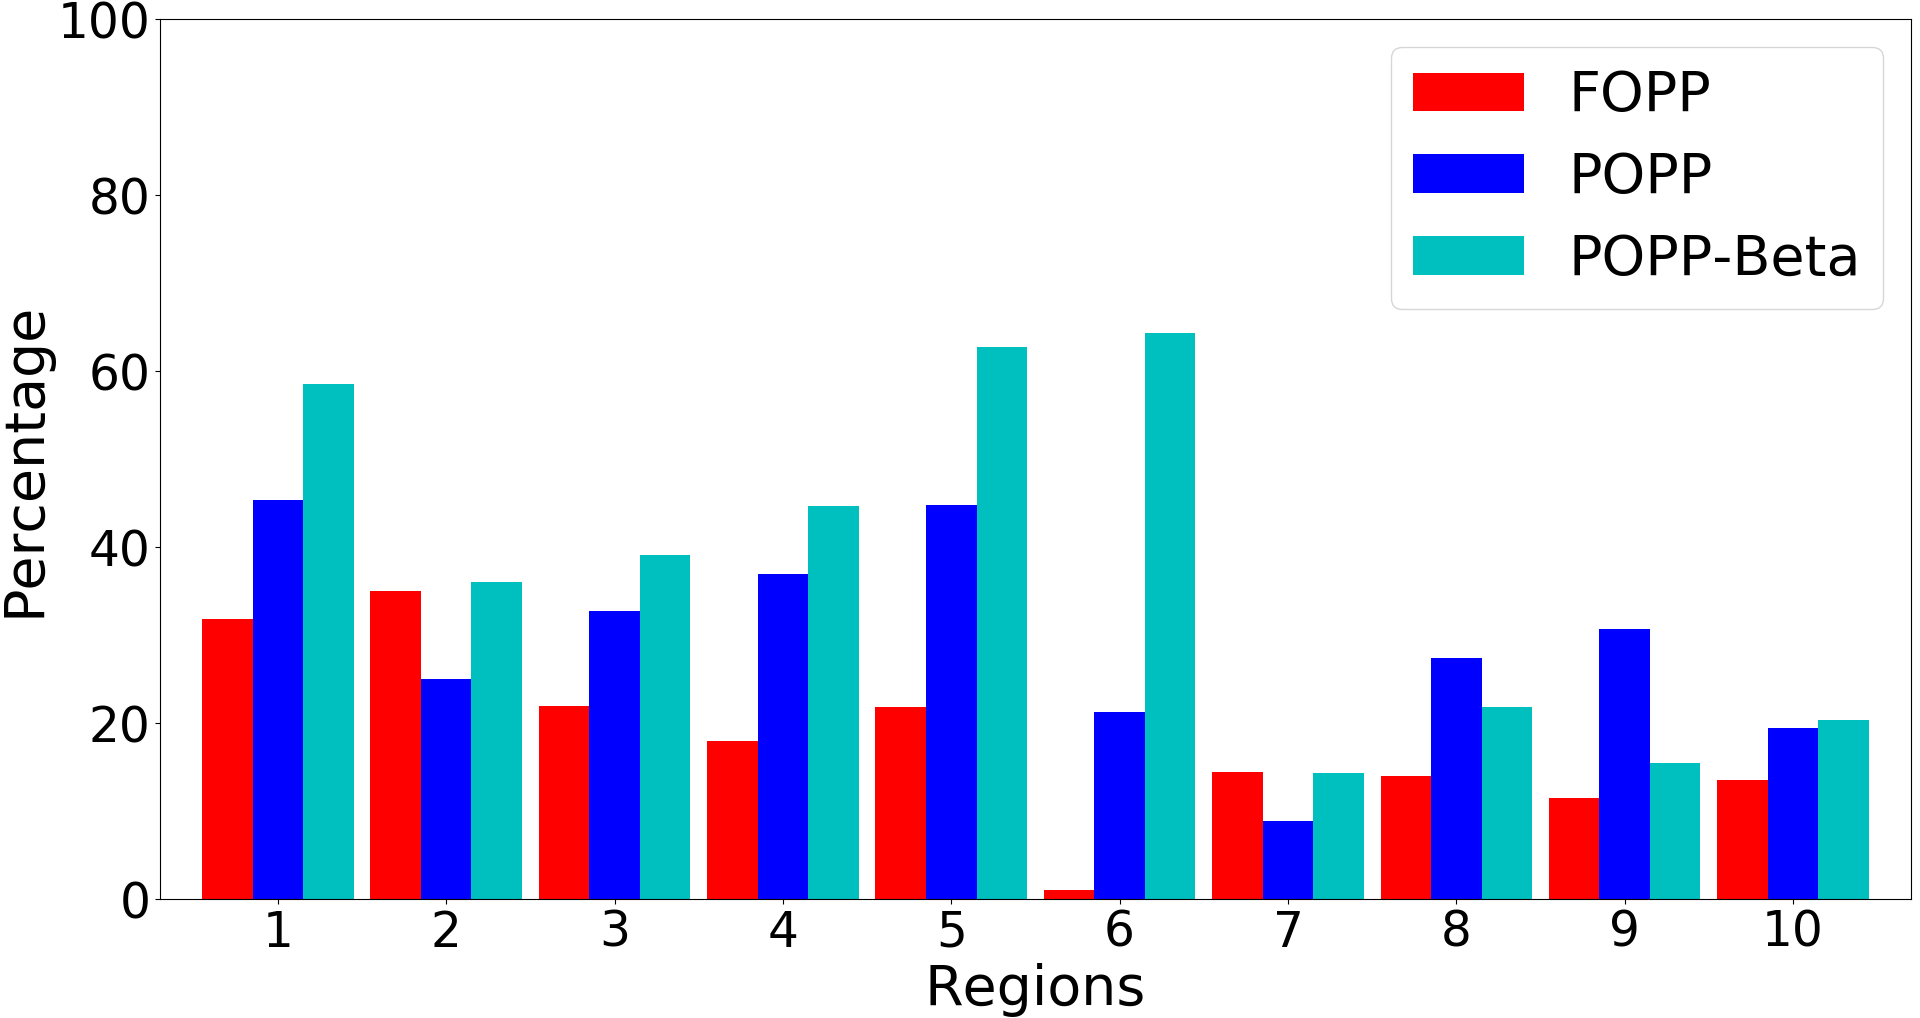
\includegraphics[width=0.5\textwidth]{./figures/exploration_percentage_region.png}
	\caption{This graph shows the percentage of time that the robot observed activities when it was present in a region. It is a measure of how successful the robot's visit policy (choice of visit time and visit location) was in finding people. It presents results for for the FOPP, POPP and POPP-algorithms. %The activity exploration percentage across areas of the environment using three different exploration models (FOPP, POPP, POPP-Beta). The percentage shows the portion of time that the robot was observing activities.
	}
	\label{fig:exploration_percentage_region}
\end{figure}

%\begin{figure}[t!]
%	\centering
%	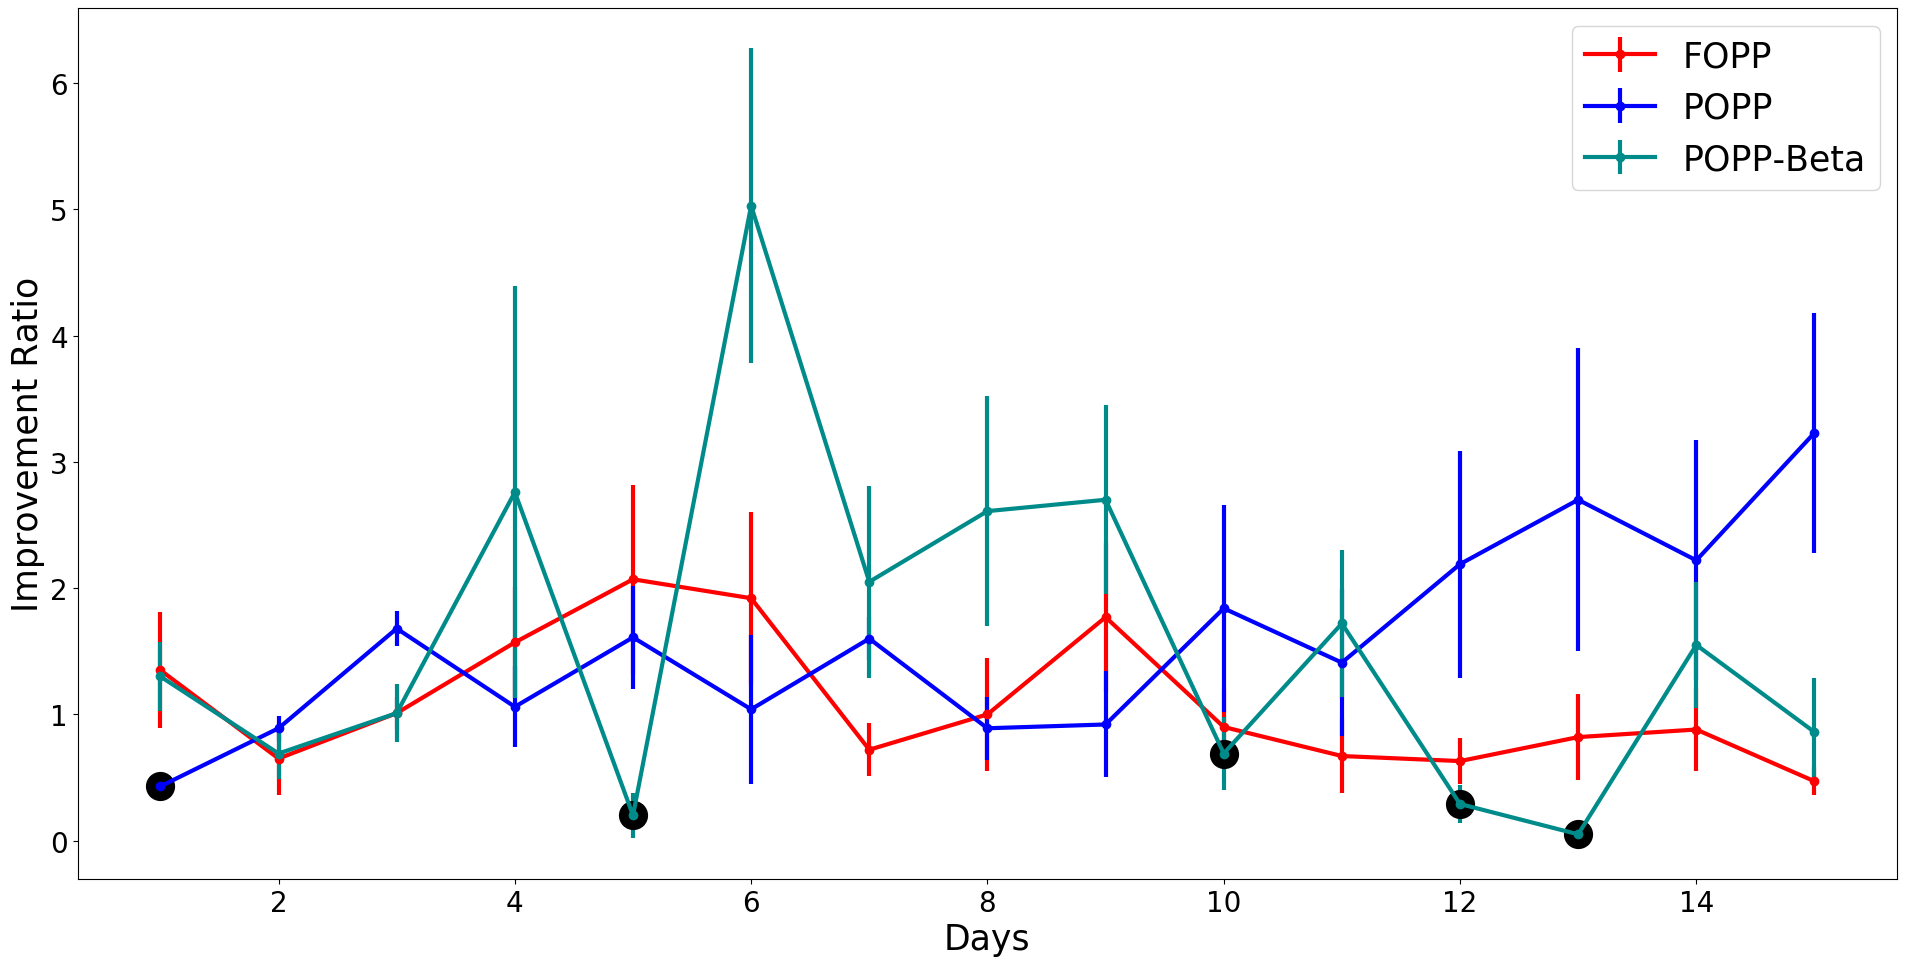
\includegraphics[width=0.5\textwidth]{./figures/exploration_improvement_ratio.png}
%	\caption{The improvement evolution of activity observation (in ratio) using three different exploration models. The average of the first three days of the number of observations on each exploration is used as the base (ratio 1.0). Black dots represent weekends the explorations were passing through.}
%	\label{fig:exploration_improvement_ratio}
%\end{figure}

%\begin{figure}[t!]
%	\centering
%	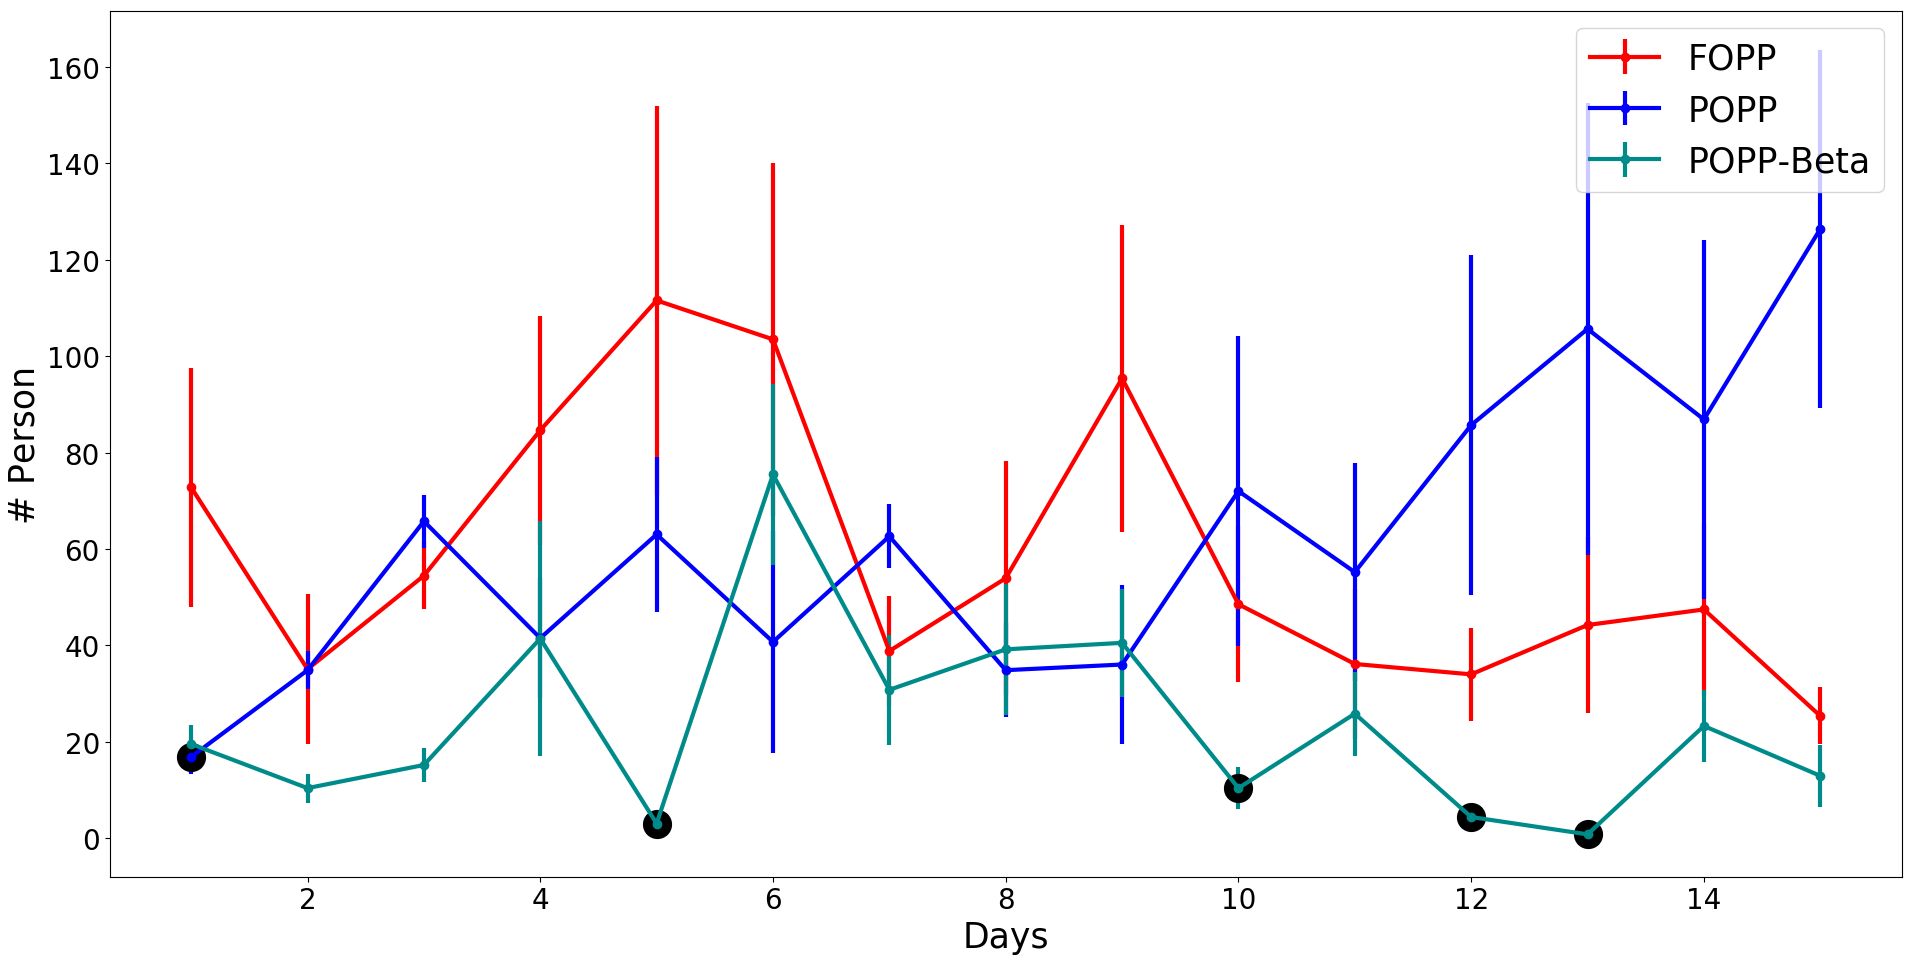
\includegraphics[width=0.5\textwidth]{./figures/exploration_number_people_across_days.png}
%	\caption{Average number of activities observed over days across regions. Black dots represent weekends the explorations were passing through.}
%	\label{fig:exploration_number_people_across_days}
%\end{figure}

\begin{figure}[t!]
	\centering
	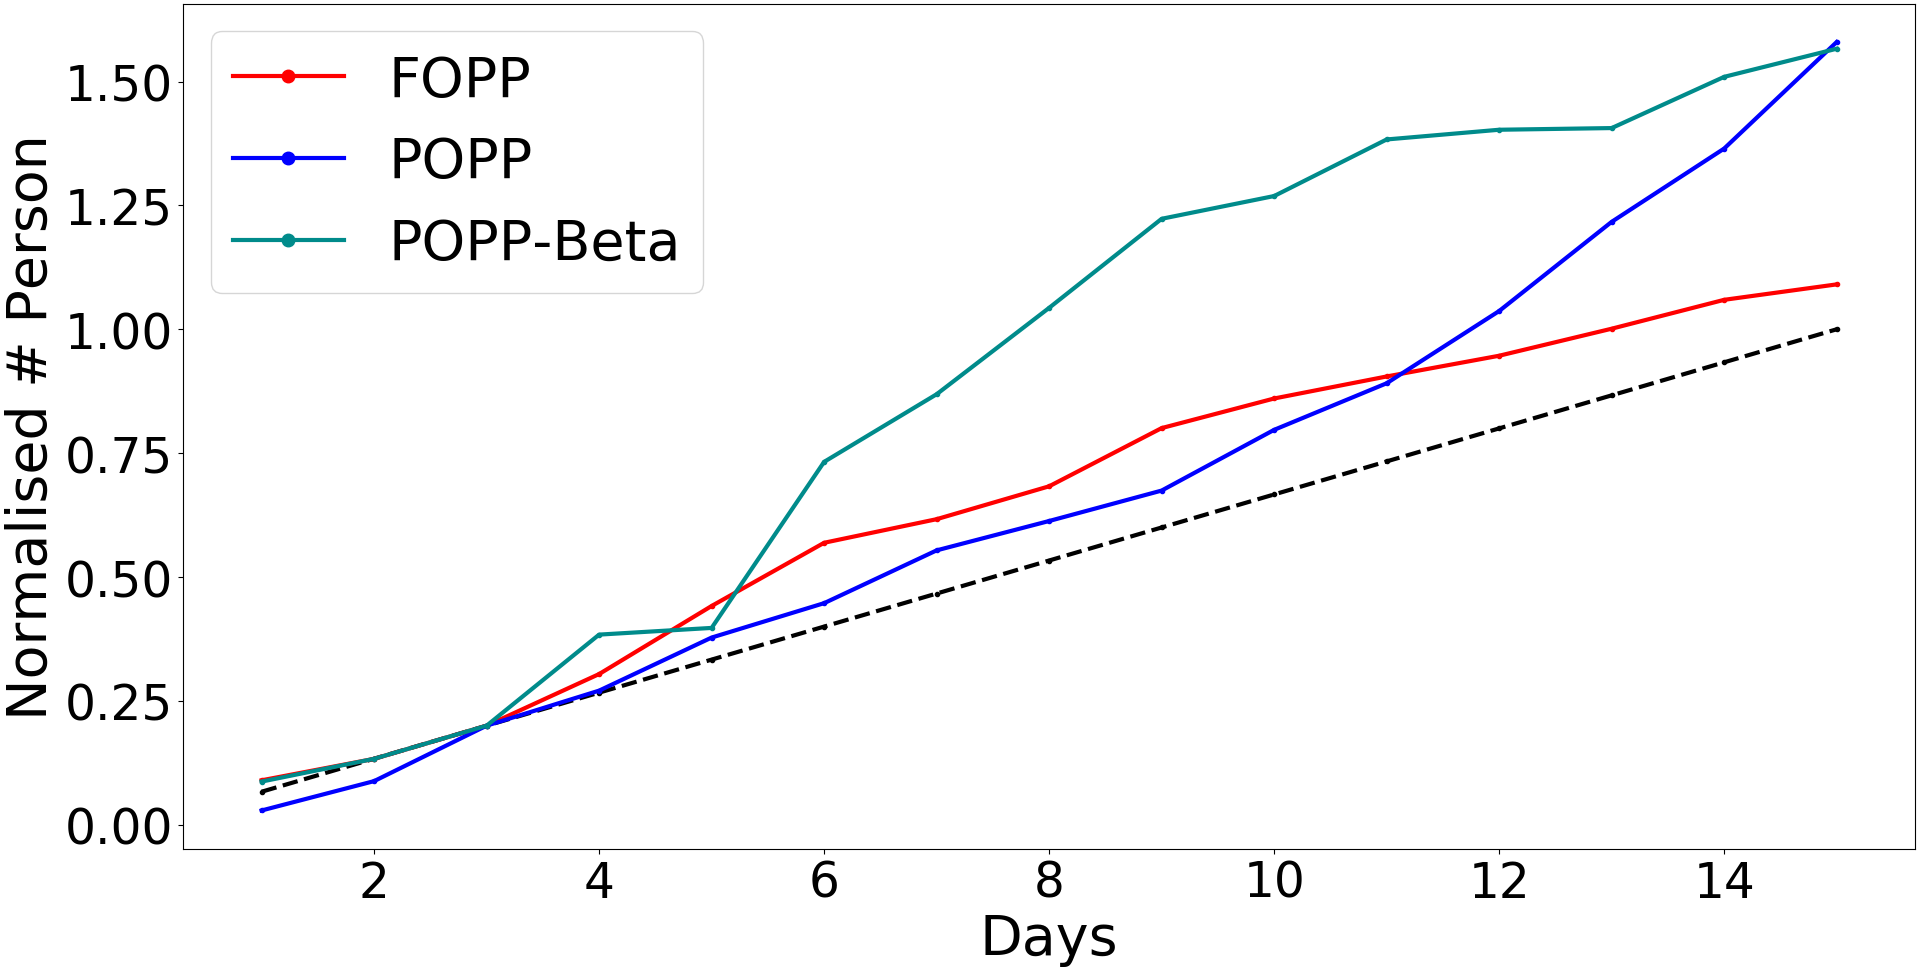
\includegraphics[width=0.5\textwidth]{./figures/exploration_number_people_across_days_normalised.png}
	\caption{The improvement ratio of activity observations during each phase of the trial. The dash line indicates a baseline performance, i.e., no improvement in exploration over time.}
	\label{fig:exploration_improvement_ratio}
\end{figure}

Figure \ref{fig:exploration_percentage_region} shows the percentage of visits to each region which yielded a non-zero true count. As can be seen, the exploration policy produced by POPP-Beta has the highest proportion of such visits in many of the regions, followed by the exploration policy according to the POPP model. Recall that some regions, such as 4, 5, 6, and 7, are not densely populated with humans across time compared to other regions (such as 1, 2, 3, and 10). The POPP and POPP-Beta models, however, still managed to improve the percentage of positive observations. This shows that the models correctly predicted that people would be present in particular locations at particular times. One should note that region 6 contains vending machines which are often detected as a person by the upper body detector. This leads to the FOPP model planning to visit this particular location when no activity is taking place. The POPP and the POPP-Beta models were able to correct the miscounts occurring in region 6, providing a better estimate of the posterior over the arrival rate $\lambda$. This leads to models that better capture the true underlying process and thus support more accurate exploration-exploitation trade-offs.

% Figure \ref{fig:exploration_number_people_across_days} shows the average number of activities observed across regions on each day. 

During the first few days of each 15 day phase the robot primarily explores since each model initially has a highly uncertain estimate of $\lambda$. As more days of data are experienced the estimates increase in confidence and the robot starts to exploit this increased confidence by visiting locations which are likely to provide higher counts\footnote{Note that this change from exploration to exploitation occurs naturally and gradually in an upper bound-based model, and therefore the characterisation of the behaviour as exploring or exploiting is a \emph{post-hoc} justification.}.
% 
To allow us to produce a metric for a fair comparison across three models (FOPP, POPP, and POPP-Beta) deployed at different times (and thus experiencing different population dynamics), we look at the ratio between the expected observations made by a baseline policy and those made by our exploration policy in the same period. 
% 
To create the baseline total for each model we take the true counts experienced for its first three days then multiply these by five to give an expected total over 15 days (the number of days of data available to every model). This is the denominator in Eqn.~\ref{eq:metric}, where $s(n)$ is the (true) number of people observed on day $n$. This is used to divide the cumulative number of observations up to the current day:

\begin{equation}
	\label{eq:metric}
\hat{s}(n) = \frac{\displaystyle\sum_{i=1}^{n} s(i)}{\displaystyle\sum_{i=1}^{3} s(i) * 5}
\end{equation}

\noindent Given this, a $\hat{s}$ score of 1.0 on day 15 shows that people have been observed people at the rate of the baseline, i.e.\ the underlying model has failed to exploit additional data correctly. A result over 1.0 shows that the model has exploited the available data to observe people at a greater rate than in the first 3 days. 
% 
Figure \ref{fig:exploration_improvement_ratio} presents the cumulative normalised true counts of people observed by the robot across the three phases. This shows that exploration driven by the POPP and the POPP-Beta models improves the number of people observed during these phases. By the end of each of these two phases, the ratio is around 1.7. On the other hand, the FOPP showed a stable ratio around the baseline (1.0 at day 15), this means that the FOPP is not be able to improve the number of people observed over time. 
% 
Also note the general trend observed earlier that the approach which represents the uncertainty in the sensor models (POPP-Beta) initially out-perform less informed approach (POPP) until the latter has observed enough of the underlying process to compensate for training inaccuracies. 

%Unfortunately for the POPP-Beta, by looking at figure \ref{fig:exploration_improvement_ratio}, we can not conclude whether the POPP-Beta can improve the number of activities observed over time.
%We argue that this is because the exploration policy produced by the Specctral-POPP-Beta was running through several weekends. We assumed of daily periodicities for the non-homogeneous Poisson processes across regions, and the assumption was broken by running the exploration throughout weekends. This is because weekdays and weekend have different arrival rate $\lambda$. Figure \ref{fig:exploration_number_people_across_days} clearly shows how small the total activities observed during weekend compared to weekdays.
%!TEX root = ../sample.tex

\section{Conclusion}
\label{sec:conclusion}

This article has presented Bayesian estimators for (1) estimating human activities, as count data, at each time of the day and (2) helping an autonomous robot optimise between exploring for new time-place combinations where it might discover a high-level of human activity and re-visiting learnt time-place combinations that a wealth of human activity is to be found. Our work was motivated by the application of counting people from an autonomous mobile robot using noisy sensors and perception algorithms. The work extends our prior work~\cite{jovan18a} with two main contributions.
% 
First, we presented variations of our previous POPP formulation: POPP-Beta extends POPP by accounting for the unreliability of the observation model; C-POPP extends POPP  by modelling the case when sensors are uncorrelated; and POPP-Dirichlet combines POPP-Beta and C-POPP to provide the benefits of each correction. Evaluations on synthetic data and observations taken by a robot show that each extension provides progressively more accurate estimates than the POPP filter.  
% 
Second, posteriors from FOPP, POPP and POPP-Beta were used to drive exploration by a mobile robot for a series of three exploration experiments. An upper bound interval exploration method in combination with Fourier transformation was used to solve the exploration-exploitation problem. This resulted in a labelled data set of of human presence counts. Our initial evaluation demonstrated that POPP and POPP-Beta were able to drive the robot to observe more people over time than the FOPP-based method. 

There are many directions for further work including utilizing C-POPP and POPP-Dirichlet to drive the robot observation in an extended time period, allowing another filter strategies for faster and more accurate posterior estimates, and removing convenient closed forms of conjugate priors in the sensor models.
        
        % Finally, the various POPP filters are compared to one another and to a FOPP estimator on this data set.

% which capture the regular structures of dynamic behaviours, especially humans,    
% 
% 
% Hence, any learning algorithm requires practical estimation which capture temporal structures of human activities.   
% 
% The adaptation requires practical estimation which capture the structure 
% 
% The robot will be able to demonstrate that it can recognise activities at various
% temporal scales, and infer or predict future activities based on its temporal model (e.g. it
% might go to the lounge because it has just seen the residents finishing their lunch). It
% will also be able to detect anomalies as sequences of very low likelihood data.
% 
% The robot only observes a limited portion of the space at any time, and so must actively plan to go to places to observe events.
% 
% learns dynamic behaviours of its surrounding while patroling around perimeters of a large area. 
% 
% Human activities follow predictable, repeating patterns that generate corresponding
% changes in space.
% 
% Our
% work will allow a robot to create a map of a building and its contents: not just walls but people,
% furniture and objects, all in a unified spatial-temporal representation that will allow a robot to
% respond robustly to the dynamics of its environment. In order to reason about the structure
% and purpose of these dynamics we will employ the spatial-temporal representations in support of
% activity recognition. This will allow the robot to detect, and exploit, patterns of human behaviour.
% 
% In our care scenario we will explore how a robot can support staff working with a small group of
% elderly patients in a nursing facility. The robot will learn about the patients’ regular activities. It
% will use this knowledge to perform support tasks for the care staff and serve as an early warning
% system when patients vary from regular behaviour (e.g. wandering the corridors at night, falling
% over). In our security scenario we will explore how a robot can act as a security guard, performing
% patrols to learn the typical spatial-temporal structures in a building and notifying a human guard
% of suspicious variations from these.

% \section{Limitations and Further Work}
% 
% Two basic statistical models: Spectral-FOPP and POPP  have been proposed and evaluated. The combination of these two is able to extract temporal dynamics in the aggregate level of human activities from unreliable sensors, along with the ability to exploit this understanding for better exploration by an autonomous mobile robot. However, the spectral-POPP model could still be improved in the following two ways:
% \begin{enumerate}
%     \item In Chapter \ref{chap:popp_independent}, The Gamma filter approximates a sum of Gamma distributions with a single Gamma distribution assuming that the sensor performs rather reliable. Instead of using a single Gamma distribution to approximate a sum of $m$ Gamma distributions, $n$ gamma distributions, where $n$ is much smaller than $m$, could be used to improve the accuracy of the approximation to the posterior. This would promise to be more accurate than a single gamma, but more efficient than a histogram filter. Thus, it might be faster than the switching filter.
% 
%     \item The spectral-Poisson model (Spectral-FOPP) in Chapter \ref{chap:spectral_poisson} is a statistical model which is able, and only able, to capture the periodic structure of count data. It indirectly assumes that there is an underlying pattern governing the evolution of the parameter $\lambda$ of a Poisson process. The spectral-Poisson might not be able to capture other non-periodic structures governing the parameter $\lambda$, such as trends. 
% 
%         A Gaussian process modulated Poisson process might provide a better model for different structures which govern $\lambda$ overtime. Work from \cite{lloyd2015variational} presents a fully variational Bayesian inference scheme for continuous Gaussian-process modulated Poisson process. It provides a good estimators and is fast in estimating $\lambda$ of a Poisson process. An extension to this statistical model which embeds both trends and periodicity in the model might provide a solution to the limitations of Spectral-Poisson while being fully Bayesian. 
% \end{enumerate}

% Listing all limitations which have been mentioned in previous sections.
% Listing all further work which can extend this thesis.

%\section*{Acknowledgment}

The research leading to these results has received funding from the European Union Seventh Framework Programme (FP7/2007-2013) under grant agreement No 600623, STRANDS. Nick Hawes was supported by UK Research and Innovation and EPSRC through the Robotics and Artificial Intelligence for Nuclear (RAIN) research hub [EP/R026084/1].


\vskip 0.2in
\bibliography{reference}
\bibliographystyle{theapa}

%!TEX root = ../sample.tex

\newpage
\appendix
\label{sec:supplementary}
\section{Sensor Model}

\begin{table}[ht]
	\centering
	\caption{Averaged sensor model for each region trained from 15 days of data.}
	\label{table:full_region_sensor_model}
	\begin{tabular}{llccc}
		\noalign{\hrule height 1.1pt}\noalign{\smallskip}
		Region & Sensor & True Negative & True Positive \\
		\noalign{\smallskip}\hline\noalign{\smallskip}
		1   & Leg               & 0.820 & 0.102 \\
		& Upper body        & 0.749 & 0.244 \\
		& Scenery change    & 0.760 & 0.612 \\ 
		2   & Leg               & 0.991 & 0.655 \\
		& Upper body        & 0.862 & 0.691 \\
		& Scenery change    & 0.826 & 0.778 \\
		3   & Leg               & 0.854 & 0.116 \\
		& Upper body        & 0.833 & 0.130 \\
		& Scenery change    & 0.780 & 0.687 \\
		4   & Leg               & 0.896 & 0.180 \\
		& Upper body        & 0.967 & 0.227 \\
		& Scenery change    & 0.897 & 0.592 \\
		5   & Leg               & 0.918 & 0.086 \\
		& Upper body        & 0.881 & 0.200 \\
		& Scenery change    & 0.877 & 0.957 \\
		6   & Leg               & 0.964 & 0.351 \\
		& Upper body        & 0.929 & 0.143 \\
		& Scenery change    & 0.803 & 0.541 \\
		7   & Leg               & 0.949 & 0.264 \\
		& Upper body        & 0.829 & 0.071 \\
		& Scenery change    & 0.939 & 0.090 \\
		8   & Leg               & 0.889 & 0.473 \\
		& Upper body        & 0.791 & 0.360 \\
		& Scenery change    & 0.900 & 0.591 \\
		9   & Leg               & 0.702 & 0.383 \\
		& Upper body        & 0.711 & 0.172 \\
		& Scenery change    & 0.591 & 0.673 \\
		10  & Leg               & 0.956 & 0.537 \\
		& Upper body        & 0.973 & 0.423 \\
		& Scenery change    & 0.823 & 0.584 \\
		%\multirow{2}{*}{Method} & \multicolumn{3}{c}{Average updating time (std. deviation)} \\
		%& 100 & 1000  & 10000 \\
		\noalign{\hrule height 1.1pt}\noalign{\smallskip}
	\end{tabular}
\end{table}

Here we provide detailed sensor models for each region. The sensor model was built from the first 15 days of data to give a general idea how each sensor performs across days. For the experiment in Section \ref{sec:evareal}, we used 48 days of data, and as we performed four fold cross validation, we only used 12 days of data to build the sensor model. During the exploration setting, only the first 3 days from 15 days of exploration for each exploration model were used to build the sensor model.

\section{Discrete Probability Distribution}

%\begin{definition2}
%	A random variable $X$ is a Bernoulli random variable with parameter $p$, i.e. $X \sim Ber(x \mid p)$, if its probability mass function is given by
%	\[
%	Ber(x \mid p) = \left\{ \begin{matrix}
%	p & \textrm{if } x = 1 \\
%	1-p & \textrm{if } x = 0 % \\
%	% 0 & \textrm{otherwise}
%	\end{matrix} \right.
%	\]
%	\noindent where $0 \leq p \leq 1$ and $x \in \{0, 1\}$.
%\end{definition2}
%
%\begin{definition2}
%	A random variable $X$ is a binomial random variable with parameter $n$ and $p$, i.e. $X \sim B(x \mid n, p)$, if its probability mass function is given by
%	\[
%	B(x \mid n, p) = \begin{pmatrix} n \\ x \end{pmatrix} p^x (1-p)^{n-x}
%	\]
%	\noindent where $0 \leq p \leq 1$ and $x \in \{0, \ldots, n\}$.
%\end{definition2}

\begin{definition2}
	A random variable $X$ is a negative binomial random variable with parameter $n$ and $p$, i.e. $X \sim NB(x \mid n, p)$, if its probability mass function is given by
	\[
	NB(x \mid n, p) = \begin{pmatrix} x - 1 \\ n - 1 \end{pmatrix} p^n (1 - p)^{x-n}
	\]
	\noindent where $0 \leq p \leq 1$ and $x \geq n$.
\end{definition2}

\begin{definition2}
	A random variable $X$ is a beta-binomial random variable with parameter $n, \zeta, \eta$, i.e. $X \sim BB(x \mid n, \zeta, \eta)$ where the $p$ parameter in the binomial distribution $B(x \mid n, p)$ is randomly drawn from a beta distribution $Be(p \mid \zeta, \eta)$ 
	\begin{equation*}
	\begin{tabular}{r@{ = }l}
	$P(x \mid n, \zeta, \eta)$ & $\displaystyle\int_{p=0}^{1} P(x \mid n, p) ~ P(p \mid \zeta, \eta) ~dp$ \\ [2ex]
	& $\displaystyle\int_{p=0}^{1} B(x \mid n, p) ~ Be(p \mid \zeta, \eta) ~dp$ \\ [2ex]
	& $\displaystyle\int_{p=0}^{1} \binom{n}{x} p^x (1-p)^{(n-x)} ~ \displaystyle\frac{p^{(\zeta - 1)} (1-p)^{(\eta-1)}}{\pi(\zeta, \eta)}$ \\ [2ex]
	& $\displaystyle\binom nx \displaystyle\frac{1}{\pi(\zeta, \eta)} ~ \displaystyle\int_{p=0}^{1} p^{(x+\zeta-1)} (1-p)^{(n-x+\eta-1)}$ \\ [2ex]
	& $\displaystyle\binom nx \displaystyle\frac{\pi(x+\zeta, n-x+\eta)}{\pi(\zeta, \eta)}$ \\ [2ex]
	& $BB(x \mid n, \zeta, \eta)$
	\end{tabular}
	\end{equation*}
\end{definition2}

\begin{definition2}
	Let $\mathbf{x}$ be a vector of $x_1, \ldots, x_m$, and $\mathbf p$ be a vector of $p_1, \ldots, p_m$. A random variable $X$ is a categorical random variable with parameter $\mathbf p$, i.e. $X \sim Cat(\mathbf x \mid \mathbf p)$, if its probability mass function is given by
	\[
	Cat(\mathbf x \mid \mathbf p) = \begin{matrix}
	p_i & \textrm{if } x_i = 1 \\
	\end{matrix}.
	\]
	\noindent where $x_i = \{0, 1\}$ and $\displaystyle\sum_{i=1}^{m} p_i = 1$.
\end{definition2}

\begin{definition2}
	Let $\mathbf{x}$ be a vector of $x_1, \ldots, x_m$, and $\mathbf p$ be a vector of $p_1, \ldots, p_m$. A random variable $X$ is a multinomial random variable with parameter $n$ and $\mathbf p$, i.e. $X \sim Multi(\mathbf x \mid n, \mathbf p)$, if its probability mass function is given by
	\[
	Multi(\mathbf x \mid n, \mathbf p) = \begin{array}{lll}
	\displaystyle \frac{n!}{x_1!, \ldots, x_m!} p^{x_1}_1 \times \ldots \times p^{x_m}_m, \\ 
	\end{array}
	\]
	\noindent where $x_i = 0, 1, \ldots$, $\displaystyle\sum_{i=1}^{m} x_i = n$, $0 \leq p_i \leq 1$, $i = 1, \ldots, m$ and $\displaystyle\sum_{i=1}^{m} p_i = 1$.
\end{definition2}

\end{document}






